%% =====================================================================
%%  manuscript.tex  --  MDPI *Remote Sensing* submission (SINGLE FILE)
%%
%%  Last updated: 2026-09-15 13:31:51
%%
%%  Everything in one file: preamble + frontmatter + 6 sections + Appendix A
%%  + internal bibliography. No \input, no subfiles.
%%
%%  Prose master (untrimmed, 9 figs / 11 tables): ../docs/manuscript.md
%%  Supplementary: ../docs/manuscript_supplementary.md
%%  Figures: figures/  (see figures/FIGURES_TODO.md)
%%
%%  OVERLEAF: start a project from the MDPI journal template (for
%%  Definitions/mdpi.cls etc.), replace its main .tex with this file,
%%  drop in figures/, set this as the Main document, compile.
%% =====================================================================

\documentclass[remotesensing,article,submit,moreauthors]{Definitions/mdpi}
% "submit" keeps line numbers on; Editorial Office flips to "accept".
% Use "preprints" as the journal key for a Preprints.org upload.

%% --- MDPI internal commands -- do not modify ------------------------
\firstpage{1}
\makeatletter
\setcounter{page}{\@firstpage}
\makeatother
\pubvolume{1}
\issuenum{1}
\articlenumber{0}
\pubyear{2026}
\copyrightyear{2026}
\datereceived{ }
\daterevised{ }
\dateaccepted{ }
\datepublished{ }

%% --- Extra packages / macros go here -------------------------------
%% (MDPI class already loads graphicx, amsmath, booktabs, tabularx,
%%  natbib, hyperref, cleveref, ... )

%% Orange-flag placeholders / not-yet-final content so they are easy to spot
%% in the compiled PDF before submission. \needsedit for short inline items
%% (names, emails, initials, a single-line statement); \needseditpar for
%% longer spans that must line-wrap (colored text only, no background box,
%% so it survives wrapping safely). Search "\needsedit" and remove both
%% definitions + all uses once every flagged item is finalized.
\usepackage{xcolor}
\newcommand{\needsedit}[1]{\colorbox{orange!40}{#1}}
\newcommand{\needseditpar}[1]{\textcolor{orange}{\bfseries #1}}

%% \path{} (from the url package, already pulled in by hyperref, but loaded
%% explicitly so it doesn't depend on hyperref's internals) typesets a
%% repository-relative file path in typewriter font and -- unlike \texttt{} --
%% allows LaTeX to break the line at "/" and "_", so long paths in the
%% Supplementary Material's "Source:" citations don't overflow the column.
%% Deliberately \path, not \url: these are internal repo paths, not web
%% URLs, so no hyperlink should be created.
\usepackage{url}

%% Centered tabularx X column. Used throughout every table in the paper
%% (main text and appendix) but NOT predefined by mdpi.cls -- the class's
%% own template shows this exact line commented out immediately above its
%% sample appendix table, to be uncommented by the author. Without it, every
%% "C" in a tabularx column spec is an undefined column-type letter, which
%% breaks column spacing/centering at compile time.
\newcolumntype{C}{>{\centering\arraybackslash}X}

%% Weighted (left-aligned) tabularx X column: L{w} takes weight w of the
%% shared elastic width; weights across a table's X columns must sum to
%% the number of X columns -- otherwise tabularx's width-fitting does not
%% resolve to \fulllength and the table renders squeezed into a fraction
%% of the line, blank space trailing it (this is what happened to Tables
%% S3/S4 below before the 2026-09-12 fix: L{2.6}CCCC / L{2.2}CCCC mixed a
%% weighted column with four *default*-weight (1) C columns, summing to
%% 6.6 / 6.2 against 5 columns, not 5). Used in Table 1 to rebalance
%% built-up/water/non-built (equal thirds wasted space on the short
%% built-up column), where all three X columns are weighted together
%% (0.45+0.90+1.65 = 3, for 3 columns) -- the working pattern to copy: when
%% one column in a row is weighted, every X column in that row must be,
%% with weights chosen to sum to the column count.
\newcolumntype{L}[1]{>{\hsize=#1\hsize\linewidth=\hsize\arraybackslash}X}

%% Weighted (centered) tabularx X column: M{w} is the centered counterpart
%% of L{w}, for rows that mix one wide text column with several narrow
%% centered numeric columns (Tables S3, S4). Same sum-to-column-count rule.
\newcolumntype{M}[1]{>{\centering\hsize=#1\hsize\linewidth=\hsize\arraybackslash}X}

%% ================= FRONTMATTER (preamble macros) ===================
%% =====================================================================
%%  body/frontmatter.tex  --  title / authors / affiliations / abstract / keywords
%%
%%  MDPI *Remote Sensing* frontmatter macros. These are PREAMBLE commands:
%%  \input this file BEFORE \begin{document} (the master docs/manuscript_body.tex
%%  chains the body sections only, from \maketitle onward).
%%
%%  Author names, ORCID, affiliation list beyond the first author, and the
%%  corresponding-author contact line are %TODO -- only the first author's
%%  centre is known.
%%
%%  Abstract trimmed to ~200 words (MDPI cap).
%%  2026-09-10: numbers refreshed for the Hangzhou two-stage standardisation
%%  (WorldCover/DW/Esri vs expert 0.47/0.45/0.42; four-way 18%; consensus
%%  0.44 vs 0.45 base rate). "WorldCover errs independently of both (Q ~ 0)"
%%  -> "at most weakly coupled to either (Q <= 0.14)".
%% =====================================================================

\Title{Cross-Product Agreement Does Not Arbitrate Reference Labels at
Land-Cover Class Boundaries: A Six-City Diagnostic}

% Short title for the running head (<= ~60 chars)
% \TitleCitation / \AuthorCitation need a recent Definitions/mdpi.cls. If your
% class errors on them ("You're in trouble here" at \TitleCitation), keep them
% commented; the class then derives the running head from \Title and the
% "How to cite" line from \Author. Re-enable after updating the Definitions/
% bundle to the current MDPI Remote Sensing template.
%% DISABLED 2026-09-12: Overleaf's mdpi.cls throws "You're in trouble here"
%% (undefined control sequence) on this -- confirmed by user compile log.
%% Class falls back to deriving the running head from \Title instead.
% \TitleCitation{Cross-Product Agreement Does Not Arbitrate the Urban Boundary Label}

% \newcommand{\orcidauthorA}{0000-0000-0000-0000} % TODO first-author ORCID

%% NOTE: \needsedit (colorbox) below is the visible title-page author list;
%% \AuthorNames is flagged with \needseditpar (color only, no box) instead
%% since some MDPI class versions reuse it in the running head, where a
%% colorbox is more likely to misbehave than plain colored text. If any
%% line here throws a compile error, that macro nesting is the first
%% suspect -- drop back to plain text and keep the surrounding % TODO.
\Author{\needsedit{Firstname Lastname} $^{1,}$*, \needsedit{Firstname Lastname} $^{2}$ and \needsedit{Firstname Lastname} $^{2}$} % TODO

\AuthorNames{\needseditpar{Firstname Lastname, Firstname Lastname and Firstname Lastname}} % TODO

%% DISABLED 2026-09-12: same undefined-control-sequence error as \TitleCitation
%% above -- confirmed by user compile log. Class falls back to the "How to
%% cite" line derived from \Author instead.
% \AuthorCitation{\needseditpar{Lastname, F.; Lastname, F.; Lastname, F.}} % TODO (needs recent mdpi.cls)

\address{%
$^{1}$ \quad \needsedit{Affiliation 1; e-mail@e-mail.com}\\ % TODO
$^{2}$ \quad \needsedit{Affiliation 2; e-mail@e-mail.com} % TODO
}

\corres{Correspondence: \needsedit{e-mail@e-mail.com}} % TODO

% \firstnote{...} % optional

%% Abstract trimmed 2026-09-10 for the MDPI ~200-word cap (was ~243 w; now
%% ~218 w). Sentence-level compression only -- every number, threshold, n-value
%% and the diagnostic/LOCO hierarchy are unchanged. Micro-wording changes to
%% flag: "used together"->"combined"; "second or third product"->"another";
%% dropped "agreed" and "(Yule's Q between their error indicators)";
%% "high everywhere"->"consistently high"; "carries a transferable signal"->
%% "is transferable". See docs/manuscript.md for the full-length version.
%%
%% 2026-09-11 -- second trim to hit the ~200 w cap exactly (was 214 w by this
%% count, now 200). Cut the LOCO sentence ("A leave-one-city-out operator
%% shows the boundary disagreement is transferable, with a bounded downstream
%% effect.") -- the only candidate identified in the 2026-09-10 pass that
%% drops a full result rather than compressing wording, chosen because LOCO is
%% already the paper's own "supporting analysis, not main contribution" per
%% [[paper-pivot-loco]]'s locked contribution skeleton; the sentence is
%% untouched in the body (sec:results-loco, sec:disc-loco) and in the C1-C5
%% list in Section 1. Also fixed "wrong toward vegetation" -> "wrong toward
%% non-built" (same overclaim as the 2026-09-11 (1) fix pass below -- Table T3
%% only supports the merged non-built class, not vegetation specifically);
%% no word-count change from that fix.
\abstract{Global 10~m land-cover products are increasingly combined on the
assumption that where independent products agree the label is close to correct,
so one product can arbitrate another's disputed pixels. We test this at
land-cover class boundaries with 900 expert-labelled points---150 in
each of six middle- and lower-Yangtze cities, China---placed by boundary-aware sampling on
the most spectrally ambiguous transitions and labelled from a 2021 Sentinel-2
composite. Only Dynamic World and Esri agree at a consistently high rate
(0.87); each matches the expert on fewer than half the points (WorldCover 0.47,
Dynamic World 0.45, Esri 0.42). That agreement is not independent
corroboration: the two products' errors move almost in lockstep (Yule's
$Q \approx 0.97$), whereas WorldCover's are at most weakly coupled to either
($Q \approx 0.08$--$0.14$). The Dynamic World--Esri consensus matches the
expert labels on 43\% of retained points, compared with 45\% for Dynamic
World alone, and all four sources agree on only 18\% of points. The
WorldCover error is directional: once WorldCover calls a point ``built-up'',
the expert label is non-built about seven times in ten. Separately, using the class agreed upon by Dynamic World and Esri as a
pseudo-label under-represents non-built cover among retained points. These
findings hold across six cities sharing one Sentinel-2 basis; cross-product
agreement should not serve on its own as a pseudo-reference or
high-confidence label at land-cover class boundaries.}

\keyword{global land-cover products; ESA WorldCover; Dynamic World; Esri Land
Cover; map agreement; correlated error; land-cover class boundary; accuracy
assessment; weak supervision; Sentinel-2}

%% ---------------------------------------------------------------------
%%  Highlights -- OBLIGATORY for Remote Sensing since 2 Sep 2025.
%%  Two questions, up to 2 bullets each; NOT a copy of the abstract.
%% ---------------------------------------------------------------------
%% Spacing note: mdpi.cls emits the label as \textbf{Highlights\vspace{-6pt}\\},
%% and after that \\ we are still in horizontal mode, so a plain \vspace here is
%% \vadjust-ed to AFTER the first question line, not above it. \mbox{}\\[len]
%% forces a genuine line break (in vertical mode) between the label and the
%% first question; tune the bracket length for the gap. The inter-question
%% \vspace and the list topsep are widened from the template defaults. Second
%% question uses the singular "main finding" wording, matching current RS
%% published articles.
\addhighlights{yes}
\renewcommand{\addhighlights}{%

\noindent\textbf{What are the main findings?}
\begin{itemize}[labelsep=2.5mm,topsep=2pt]
\item At land-cover class boundaries in six middle- and lower-Yangtze cities,
none of ESA WorldCover, Dynamic World or Esri matches expert labels on even half
the boundary points (0.47, 0.45, 0.42), and the Dynamic World--Esri consensus does no better
(0.43 vs.\ a 0.45 base rate).
\item The only agreement that is high across all six cities, Dynamic World with
Esri (0.87), is correlated error rather than independent corroboration: their
errors move almost in lockstep (Yule's $Q \approx 0.97$, against $\approx 0.08$--$0.14$ for
either WorldCover pair).
\end{itemize}\vspace{10pt}
\noindent\textbf{What is the implication of the main finding?}
\begin{itemize}[labelsep=2.5mm,topsep=2pt]
\item At land-cover class boundaries, cross-product agreement should not be used on its
own as a pseudo-reference, a high-confidence training label, or a quality
filter. The WorldCover error is directional: once WorldCover calls a point
``built-up'', the expert label is non-built about seven times in
ten---and, separately, agreement-filtered
(Dynamic World--Esri) labels also under-represent non-built cover among the
points retained.
\item Product disagreement is itself informative and transfers across cities (a
leave-one-city-out operator), so it can instead be used to target expert review.
\end{itemize}
}

\begin{document}

\maketitle

%% ===================== 1  INTRODUCTION ============================
%% =====================================================================
%%  body/intro.tex  --  Section 1 (Introduction + Related Work)
%%  Drop-in fragment; compiles only inside the MDPI Remote Sensing template.
%%
%%  2026-09-13 -- contribution list collapsed from five to four. Former C4
%%  (leave-one-city-out check, previously its own numbered item reading as a
%%  method/process -- "a leave-one-city-out correction operator showing...")
%%  folded into C2 as a robustness clause ("the pattern is not a single-city
%%  artifact, since a leave-one-city-out check reproduces the same signal...").
%%  Former C5 renumbered C4; back-reference "the C5 practice..." in the
%%  Discussion (sec:disc-edge area) updated to "C4". Abstract, Highlights,
%%  and the Appendix S6 "(C1/C2)" captions do not use the letter numbering
%%  past C2 and are unaffected. See [[paper-pivot-loco]] in project memory.
%%  Trailing ", with a bounded downstream footprint" cut from the C2 clause
%%  same day: it described the operator's limited effect on a downstream
%%  classifier, not evidence that the pattern generalises across cities, so
%%  grafted onto the "not a single-city artifact, since..." clause it read as
%%  a non sequitur. The point itself is intact in sec:disc-loco ("the right
%%  scale for auditing a label map, not for retraining one").
%%
%%  2026-09-10 — readability pass (sentence-level only). Split long
%%  multi-clause sentences; no claim, number, citation, contribution label
%%  (C1-C5, historical at time of that pass) or cross-reference changed;
%%  every edit information-equivalent.
%%  Edits: para 1 "whole-map averages" sentence split; para 2 "seldom
%%  stated ... arbitrate a disputed pixel" split; para 3 "a test that
%%  separates ..." split; contribution C1 split at "showing that"; Related
%%  Work "Labels derived from existing maps" PRE sentence split in two.
%%  Contribution wording, Related-Work citations, and "The gap" enumeration
%%  unchanged.
%%
%%  2026-09-10 (b) — structural + clarity. Demoted the "Related Work"
%%  subsection to running text: removed \subsection{Related Work} and its
%%  \label{sec:relwork} (no \ref referenced it anywhere in the manuscript);
%%  the three \paragraph run-in headings now carry the structure, so
%%  Section 1 no longer has a lone 1.1. Clarity edits, information-equivalent,
%%  no claim/number/citation/contribution label changed: para 2 "is taken to
%%  arbitrate" -> "is assumed to arbitrate" (echoes "that assumption" in the
%%  next sentence); para 5 "but a region where" -> "but it is a region where"
%%  (re-anchors the "is not ... but ..." parallel across the em-dash clause).
%%
%%  Cite keys: venter2022 xu2024 yuan2026 tuanmu2014 zhangroy2017 wang2024a
%%             wang2024b chakraborty2024 tong2024pre
%%  Labels defined: sec:intro   (sec:relwork removed 2026-09-10b)
%%  Labels expected: sec:results-independence sec:loco
%% =====================================================================

\section{Introduction}\label{sec:intro}

Global 10~m land-cover products---ESA WorldCover, Google/WRI Dynamic World, and
Esri/Impact Observatory Land Cover---are now routine inputs to urban and
environmental analysis, distributed ready-to-use on cloud platforms and cited
with headline overall accuracies in the 70--90\% range
\citep{venter2022,xu2024}. Those headline figures are whole-map averages. They
hide a well-documented weak spot: the transition between built-up land and
vegetation, where mixed pixels, spectral similarity and differing class
definitions push the products apart from one another and from field observation
\citep{xu2024,yuan2026}. Intra-urban green space---parks, street trees,
residential and campus greenery embedded in the built matrix---is absorbed into
the built class by several products, a bias large enough to matter for the
urban-ecology and planning applications that consume these maps
\citep{yuan2026}.

A common response to this uncertainty, where independent reference data are
scarce or costly, is to lean on several products at once. Pixels on which
multiple independent products agree are treated as reliable: merged into
accuracy-weighted consensus layers \citep{tuanmu2014}, used as pseudo-reference
for accuracy assessment, or harvested as high-confidence training and
validation samples for new classifications \citep{zhangroy2017,wang2024a}. The
step is convenient and intuitive, and it rests on an assumption that is seldom
stated, let alone tested: that where independent products agree, the agreed
label is close to correct. By extension, consulting a second or third product
is assumed to arbitrate a disputed pixel. Whether that assumption holds at
land-cover class boundaries, the very place the products are weakest,
has not been examined. The product-comparison literature reports how far the
maps sit from reference data on average, but not whether their mutual agreement
is independent corroboration or shared error, and not specifically on boundary
pixels.

Testing it requires two things the standard comparisons do not provide. First,
reference labels placed on the contested pixels rather than spread across a
globally representative sample, so that the hard cases are not diluted to a
handful of points. Second, a test that separates agreement-as-corroboration
from agreement-as-correlated-error. Two products may agree because both are
right; two others may agree because they share a model family, a training
corpus or a preprocessing chain. The two cases look identical in a pairwise
agreement table but carry opposite implications for arbitration.

This paper supplies both, for six cities in the middle and lower reaches of the Yangtze River in China
(Wuhan, Hefei, Nanchang, Nanjing, Changsha, Hangzhou). A boundary-aware
sampling step spends a deliberately small photo-interpretation budget---900
points, 150 per city---on the most spectrally ambiguous land-cover class
transitions, each labelled by expert interpretation of a 2021 Sentinel-2
composite. On these points we (i)~quantify how far ESA WorldCover, Dynamic
World and Esri Land Cover depart from the expert labels and from one another;
(ii)~test directly whether a second and third product arbitrate the
disagreement, formalising the test as whether product predictions are
conditionally independent given the expert label and reporting the joint error
structure of the three
products; (iii)~characterise the direction of the WorldCover error and the
physical scenes in which the disagreement concentrates; and (iv), as a
supporting analysis, ask with a leave-one-city-out correction operator whether
the disagreement carries a signal that transfers to a city whose own labels
were withheld entirely.

The scope is stated plainly. The boundary-candidate population spans each
city's full administrative area and every pairwise transition in the
three-class scheme. The three classes are built-up, non-built and water;
non-built includes vegetation, cropland and bare land. The results
below concentrate on the built-up/non-built pairing because that is where the
products disagree most and where downstream weak-supervision pipelines are
most exposed. The six cities are one country, one climate, one
broad urban-build morphology, and one shared Sentinel-2 information base;
every rate reported here is
conditional on a boundary-candidate population and is not a map-wide accuracy
of any product. The result shows the behaviour exists within that domain,
not how often it occurs elsewhere. The middle and
lower Yangtze is not an easy case---it is one of the harder land-cover settings---but it is
a region where the monitoring demand is concrete.

This paper makes four contributions. \textbf{C1}, the central one, is a direct
test of an assumption that is widely relied on but seldom examined---that
agreement among global products is evidence of correctness, so that a second or
third product can arbitrate a disputed pixel. At land-cover class
boundaries, in these six cities, it can fail: the Dynamic World--Esri
consensus does not clearly exceed the single-product base rate, and the two
products that agree
most (Dynamic World and Esri) err together while WorldCover's errors are at most
weakly coupled to either, so their agreement is correlated error rather than
independent corroboration.

\textbf{C2}: two related but distinct findings at the boundary. WorldCover's
error is directional, not symmetric noise---once WorldCover calls
``built-up'', the expert reads non-built about seven times in ten; the
pattern is not a single-city artifact, since a leave-one-city-out check
reproduces the same signal in a city whose own labels were withheld
entirely.
Separately, using the class agreed upon by Dynamic World and Esri as a
pseudo-label systematically under-represents non-built cover among retained
points.

\textbf{C3}: the
boundary-aware sampling step, offered as a practical and reproducible way to
spend a small photo-interpretation budget on the hard pixels, not as a new
active-learning method.

\textbf{C4}: the resulting methodological caution---%
cross-product agreement should not be used on its own as a pseudo-reference, a
high-confidence label source, or a quality filter, because the spectral and
temporal safeguards in current weak-supervision pipelines are not designed to
catch error that is correlated across the products being combined.

\paragraph{Product inter-comparison.} Several studies benchmark the 10~m global
products against independent ground data. \citet{venter2022}, in this journal,
compare Dynamic World, WorldCover and Esri Land Cover at a global reference
sample (overall accuracy on their scheme: Esri $\approx$ 75\%, Dynamic World
$\approx$ 72\%, WorldCover $\approx$ 65\%) and document systematic per-class
biases; they also record the definitional split that matters here---Dynamic
World's built-area predictions can incorporate urban vegetation and green
space in practice, whereas WorldCover's nominal Built-up class
excludes it. \citet{xu2024} run a comparative
independent validation of the same three maps, with overall accuracies of
73--83\% depending on how reference-data uncertainty is handled.
\citet{wang2024b} evaluate six high-resolution products over China and find
inter-product consistency running below per-product accuracy.
\citet{chakraborty2024} show large disagreements between products in estimates
of urban land \emph{area}, driven by scale and differing urban definitions.
Together these establish that the products disagree; none focuses on boundary
pixels, places reference labels on the hard cases by design, or tests whether
product agreement functions as arbitration.

\paragraph{Labels derived from existing maps.} A parallel line of work treats
existing maps as a label source. \citet{zhangroy2017} use the 500~m MODIS
land-cover product to derive training labels for a 30~m Landsat classification;
\citet{wang2024a} fuse several 10~m products by weighted majority vote into a
training-sample pool, with a downstream spectral-outlier filter;
\citet{tong2024pre} train a global high-categorical-resolution map by weak
supervision from existing products. These pipelines operationalise the
agreement-as-reliable-label assumption that Section~\ref{sec:results-independence}
tests. The same paper's within-region prototype\,/\,pseudo-label
rectification-and-expansion approach (``PRE'') propagates sparse labels to
their feature neighbours. We adapted it to a within-city setting during this
project and found that it leaks under spatial autocorrelation once evaluation
points are properly held out (Section~\ref{sec:loco}), which is why the
correction operator here is trained across cities with the target city entirely
excluded.

\paragraph{The gap.} No existing study combines (i)~a boundary-pixel focus
rather than a whole-map average, (ii)~active sampling that places a small
manual budget precisely on land-cover class transitions, and (iii)~an
explicit test of whether product predictions are conditionally independent
given the expert label, supported by the joint error structure of the
three products, with checks on class ontology, shared imagery and acquisition
date narrowing but not fully separating the space of explanations.
\emph{Why} the two products are coupled is left as a
hypothesis for the Discussion, not asserted as a result.

%% ===================== 2  STUDY AREA AND DATA =====================
%% =====================================================================
%%  body/studyarea.tex  --  Section 2 (Study Area and Data)
%%  Drop-in fragment; compiles only inside the MDPI Remote Sensing template.
%%
%%  2026-09-10 — readability pass (sentence-level only). Split long
%%  multi-clause sentences; no claim, number, citation or cross-reference
%%  changed; first-author pronoun ("she") left as written by the authors;
%%  table, caption and legend crosswalk untouched. Every edit
%%  information-equivalent.
%%
%%  Cite keys: yang2021land liao2025 yu2023 tong2024land lu2026 zhao2026
%%             fao2015gaul gorelick2017 zanaga2022 brown2022 karra2021 venter2022
%%  Labels defined: sec:data sec:studyarea sec:aoi sec:products sec:annotators
%%                  tab:legend_map
%%  Labels expected: fig:studyarea sec:sampling sec:diagnostic sec:disc-edge
%%                   sec:disc-scope app:recheck
%% =====================================================================

\section{Study Area and Data}\label{sec:data}

\subsection{Study Area}\label{sec:studyarea}

The study covers six provincial capitals in the middle and lower reaches of the
Yangtze River in China---Wuhan (Hubei), Hefei (Anhui), Nanchang (Jiangxi),
Nanjing (Jiangsu), Changsha (Hunan) and Hangzhou (Zhejiang)
(Figure~\ref{fig:studyarea}). The region has urbanised rapidly over the past
three decades, with built-up land expanding largely at the expense of cropland
and water \citep{yang2021land,liao2025}. It also falls under several
overlapping land-management regimes---ecological protection red lines,
permanent basic farmland protection, and shoreline and flood-detention
controls---that all rely on accurate, repeatable land-cover monitoring
\citep{yu2023,tong2024land}. It is not an easy classification setting: paddy,
aquaculture ponds and wetland interleave finely with the built and vegetated
classes, mixed pixels are common at 10~m, and the built-up/vegetation
transition---the focus of this study---is among the boundaries global products
place least reliably \citep{lu2026,zhao2026}. The six cities were selected
because this monitoring demand is concrete. They are not put forward as a
globally representative sample (Section~\ref{sec:disc-scope}).

\begin{figure}[H]
\begin{adjustwidth}{-\extralength}{0cm}
\centering
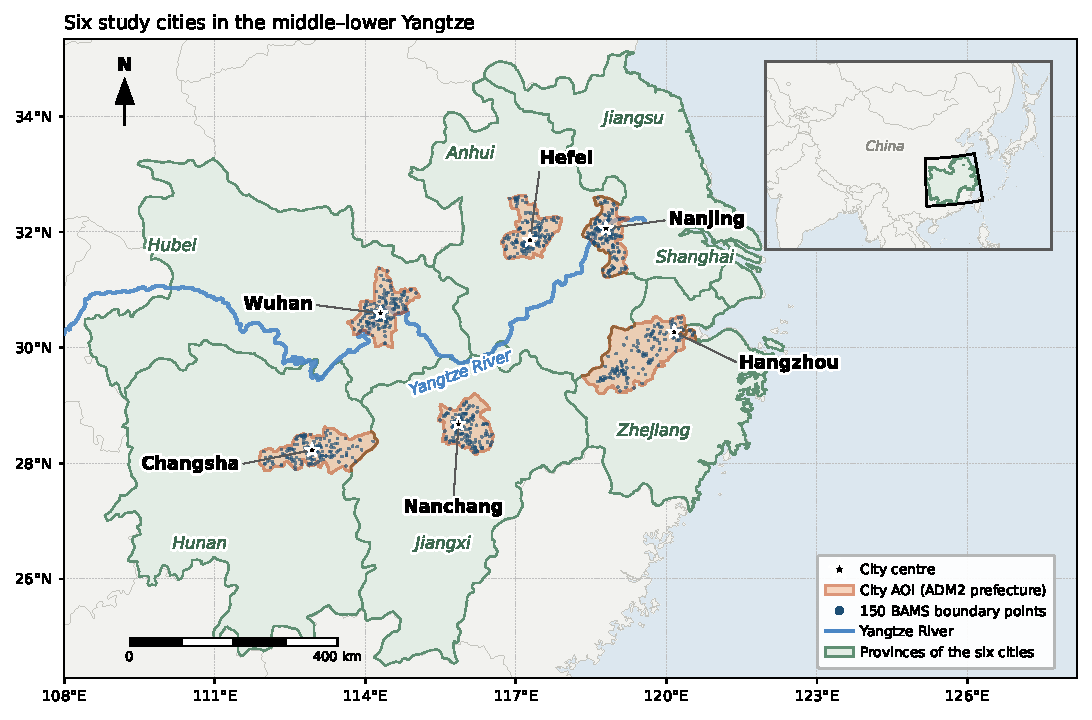
\includegraphics[width=\linewidth]{figures/Figure1_study_area.pdf}
\end{adjustwidth}
\caption{Study area. The six provinces containing the study cities are named,
with the Yangtze River main stem drawn in; each city's area of interest is its
FAO GAUL 2015 level-2 (prefecture) polygon \citep{fao2015gaul}, filled and
outlined, with its 150 boundary-candidate points plotted inside. The unlabelled
inset locates the study region within East Asia: every country in the region is
drawn with its own national border in the same uniform style, with the six
study provinces highlighted and the main map's extent boxed.
\label{fig:studyarea}}
\end{figure}

\subsection{Area of Interest and Sentinel-2 Basis}\label{sec:aoi}

For each city the area of interest is the whole second-level administrative unit
(FAO GAUL 2015, ADM2---the prefecture-level municipality;
\citealp{fao2015gaul}), taken in full with no built-up or urban mask, so the
candidate pool spans the built-up core together with the surrounding rural
land. All spectral inputs come from a single 2021 Sentinel-2
surface-reflectance composite per city, built from
\href{https://developers.google.com/earth-engine/datasets/catalog/COPERNICUS_S2_SR_HARMONIZED}{\path{COPERNICUS/S2_SR_HARMONIZED}} over the full calendar year (scenes
below 20\% cloud, per-pixel median). From it we take six bands (B2, B3, B4, B8,
B11, B12) and three indices (NDVI, NDBI, MNDWI), each also summarised over a
$3 \times 3$ pixel neighbourhood. The same composite is the primary reference
imagery for the expert labelling. The compositing recipe, the stratified
candidate pool and the boundary-aware selection are given in
Section~\ref{sec:sampling}. All image processing was carried out in Google
Earth Engine \citep{gorelick2017}.

\subsection{Global Land-Cover Products}\label{sec:products}

Three global 10~m land-cover products are compared, all for the 2021 epoch.

\begin{itemize}[leftmargin=*]
\item \textbf{ESA WorldCover v200} \citep{zanaga2022}---an annual
  gradient-boosted-tree classification of Sentinel-1 and Sentinel-2 with a
  rule-based post-process. WorldCover has a dual role here: its remapped classes
  drive the stratified candidate pool (Section~\ref{sec:sampling}), and it is
  one of the three references in the diagnostic.
\item \textbf{Dynamic World} \citep{brown2022}---a near-real-time deep
  semantic-segmentation model on Sentinel-2; we take the 2021 annual mode of
  the class band (\href{https://developers.google.com/earth-engine/datasets/catalog/GOOGLE_DYNAMICWORLD_V1}{\path{GOOGLE/DYNAMICWORLD/V1}}).
\item \textbf{Esri\,/\,Impact Observatory Land Cover} \citep{karra2021}---an
  annual deep semantic-segmentation model on Sentinel-2; we take the 2021 layer
  of the time-series product (\href{https://gee-community-catalog.org/projects/S2TSLULC/}{\path{ESRI_Global-LULC_10m_TS}}).
\end{itemize}

Each product's native legend is collapsed to the same three classes used for
the expert labels---built-up, non-built, water---as set out in
Table~\ref{tab:legend_map}.

\begin{table}[H]
\caption{Legend crosswalk from each product's native classes to the three-class
scheme. Wetland and flooded\,/\,inundated vegetation are assigned to
\textbf{water} for all three products, a deliberate and consistent ontology
choice for this wetland- and aquaculture-rich region. Esri's ``Clouds'' class
(code 10) is treated as no-data and excluded. The same three-class WorldCover
remap defines the stratified candidate pool (Section~\ref{sec:sampling}).\label{tab:legend_map}}
\begin{adjustwidth}{-\extralength}{0cm}
\footnotesize
\begin{tabularx}{\fulllength}{l L{0.45} L{0.90} L{1.65}}
\toprule
\textbf{Product (native classes)} & \textbf{$\to$ built-up} & \textbf{$\to$ water}
& \textbf{$\to$ non-built}\\
\midrule
\textbf{ESA WorldCover v200} (11) & 50 Built-up & 80 Permanent water, 90
Herbaceous wetland, 95 Mangroves & 10 Tree cover, 20 Shrubland, 30 Grassland,
40 Cropland, 60 Bare\,/\,sparse vegetation, 70 Snow and ice, 100 Moss and
lichen\\
\addlinespace
\textbf{Dynamic World} (9) & 6 Built & 0 Water, 3 Flooded vegetation & 1 Trees,
2 Grass, 4 Crops, 5 Shrub and scrub, 7 Bare, 8 Snow and ice\\
\addlinespace
\textbf{Esri\,/\,Impact Observatory 2021} (9) & 7 Built Area & 1 Water, 4
Flooded vegetation & 2 Trees, 5 Crops, 8 Bare ground, 9 Snow\,/\,Ice, 11
Rangeland\\
\bottomrule
\end{tabularx}
\end{adjustwidth}
\end{table}

The schemas differ at the boundary in a way that matters for this study:
Dynamic World's built-area predictions can incorporate urban vegetation and
green space in practice, whereas WorldCover's nominal Built-up class excludes
vegetation
\citep{venter2022}. This split is taken up again in
Section~\ref{sec:disc-edge}. WorldCover enters every analysis; Dynamic World
and Esri enter only the four-way agreement and the independence diagnostic
(Section~\ref{sec:diagnostic}), and the correction-operator referee
(Section~\ref{sec:loco}).

\subsection{Annotators}\label{sec:annotators}

All 900 reference points were interpreted by the first author, a remote-sensing
analyst at the Land Satellite Remote Sensing Application Center, Ministry of
Natural Resources of China. In that role she is responsible for
satellite-imagery coordination and provision across the ministry's
natural-resources system, and she carries out applied research on
feature-based land-cover classification from high-resolution optical imagery,
including multi-feature cloud and snow detection. The reliability exercise of
Section~\ref{sec:sampling} was carried out by three of her colleagues at the
same centre (denoted A, B and C; not authors of this study), each with more
than ten years of operational satellite-image interpretation experience and
none of whom took part in the original labelling. The blind re-check of
Appendix~\ref{app:recheck} was done by one of the three. This operational and
research experience is what made a single consistent reference feasible on the
boundary candidates. It is an enabling condition for the reference, not a
rationale for the choice of study area (Section~\ref{sec:studyarea}), and the
resulting single-annotator reference is treated as a limitation in
Section~\ref{sec:disc-scope}.

%% ===================== 3  METHODS ================================
%% =====================================================================
%%  body/methods.tex  --  Section 3 (Methods)
%%  Drop-in fragment; compiles only inside the MDPI Remote Sensing template.
%%
%%  2026-09-10 — readability pass (sentence-level only). Principle for this
%%  manuscript: maximise human readability without losing rigour. Edits:
%%  split long multi-clause sentences; cut meta-commentary; de-nominalise;
%%  unpack multi-clause parentheticals. NOT changed: any claim, number,
%%  threshold, n-value, statistic, citation key, equation, cross-reference,
%%  defined term (margin, BoundaryScore, correction operator, "the operator
%%  fires", BAMS150, "conditional on that population"), load-bearing
%%  qualifier (in-sample, conservative lower bound, "does not require the
%%  expert label to be ground truth"), or the diagnostic(main)/LOCO
%%  (supporting) hierarchy. Every edit checked for information-equivalence.
%%  Edits by subsection: intro/caveat -> one ";" split each; 3.1 candidate
%%  pool -> prefecture/rural-land sentence split in three; 3.1 inputs ->
%%  composite parenthetical unpacked into a lead + recipe sentence; 3.1
%%  boundary-score preamble -> ";" split; enumerate item 1 -> one split,
%%  "(no neighbourhood terms ...)" -> clause; post-enumerate -> "is only a
%%  proposal mechanism for isolating spectrally ambiguous zones" -> "serves
%%  only to isolate spectrally ambiguous zones for annotation"; 3.1
%%  selection -> long sentence split after "fixed to it"; 3.1 expert
%%  labelling -> rendering/basemap ";" split, reliability sentence split in
%%  two; 3.1 sampling-induced conditioning -> em-dash parenthetical made
%%  its own sentence; 3.2 reference layers -> product colon-list -> three
%%  sentences + second paragraph; 3.2 (b),(d),(e) -> meta-phrases trimmed,
%%  ";" splits; 3.3 design rationale -> PRE sentence split, "which removes
%%  this dependence" -> "This removes the dependence"; 3.3 operator ->
%%  27-feature parenthetical unpacked, "firing is further restricted by a
%%  boundary gate" -> "a boundary gate further restricts firing"; 3.4
%%  spatial-block / controls / reproducibility -> ";" splits. (c), metrics,
%%  target-city isolation, fixed-classifier: unchanged.
%%
%%  Cite keys: fao2015gaul zanaga2022 gorelick2017 landis1977 brown2022
%%             karra2021 wilson1927 yule1900 tong2024pre
%%  Labels defined: sec:methods sec:sampling sec:diagnostic sec:loco
%%                  eq:margin eq:bscore eq:netbuilt eq:condindep eq:be
%%  2026-09-10: Hangzhou standardised onto the two-stage rule (Eq. hzblend +
%%  the "five of six / weighted-blend" para removed; 104 points re-labelled).
%%  2026-09-11 — external-review fix pass (Remote_Sensing_投稿评估.md): (S2c)
%%  arbitration-value exception to "does not require the expert label to be
%%  ground truth" now flagged inline at first mention (was previously stated
%%  as a blanket claim; the exception was already correct in
%%  Section~sec:disc-scope but not cross-referenced back to here). "Conservative
%%  lower bound" for the excess-agreement in-sample bias reworded to "expected
%%  to understate the true value" -- same claim, hedge made explicit rather than
%%  asserted as a guarantee. Neither change alters any reported number.
%%  Labels expected: fig:flowchart fig:independence tab:legend_map tab:T1 tab:T2
%%                   tab:T3 tab:T4 tab:S1 tab:S2 sec:results
%%                   sec:results-confidence sec:results-independence
%%                   sec:disc-scope sec:studyarea sec:annotators
%% =====================================================================

\section{Methods}\label{sec:methods}

The analysis has three stages, summarised in Figure~\ref{fig:flowchart}. First,
a boundary-aware sampling step (Section~\ref{sec:sampling}) spends a small
photo-interpretation budget on the pixels where global products are most likely
to depart from expert judgement; it produces 900 hand-labelled boundary points
across six cities. Second, a multi-reference agreement diagnostic
(Section~\ref{sec:diagnostic}) quantifies \emph{how much}, \emph{where}, and
\emph{in which direction} ESA WorldCover, Dynamic World and Esri Land Cover
disagree with the expert labels, and tests directly whether consulting a second
and a third product resolves the disagreement. Third, as a supporting analysis,
a leave-one-city-out (LOCO) correction operator (Section~\ref{sec:loco}) asks
whether the expert corrections learned on five cities transfer to a sixth city
that contributes no labels of its own, together with the evaluation protocol
and leakage controls specific to that test.

\begin{figure}[H]
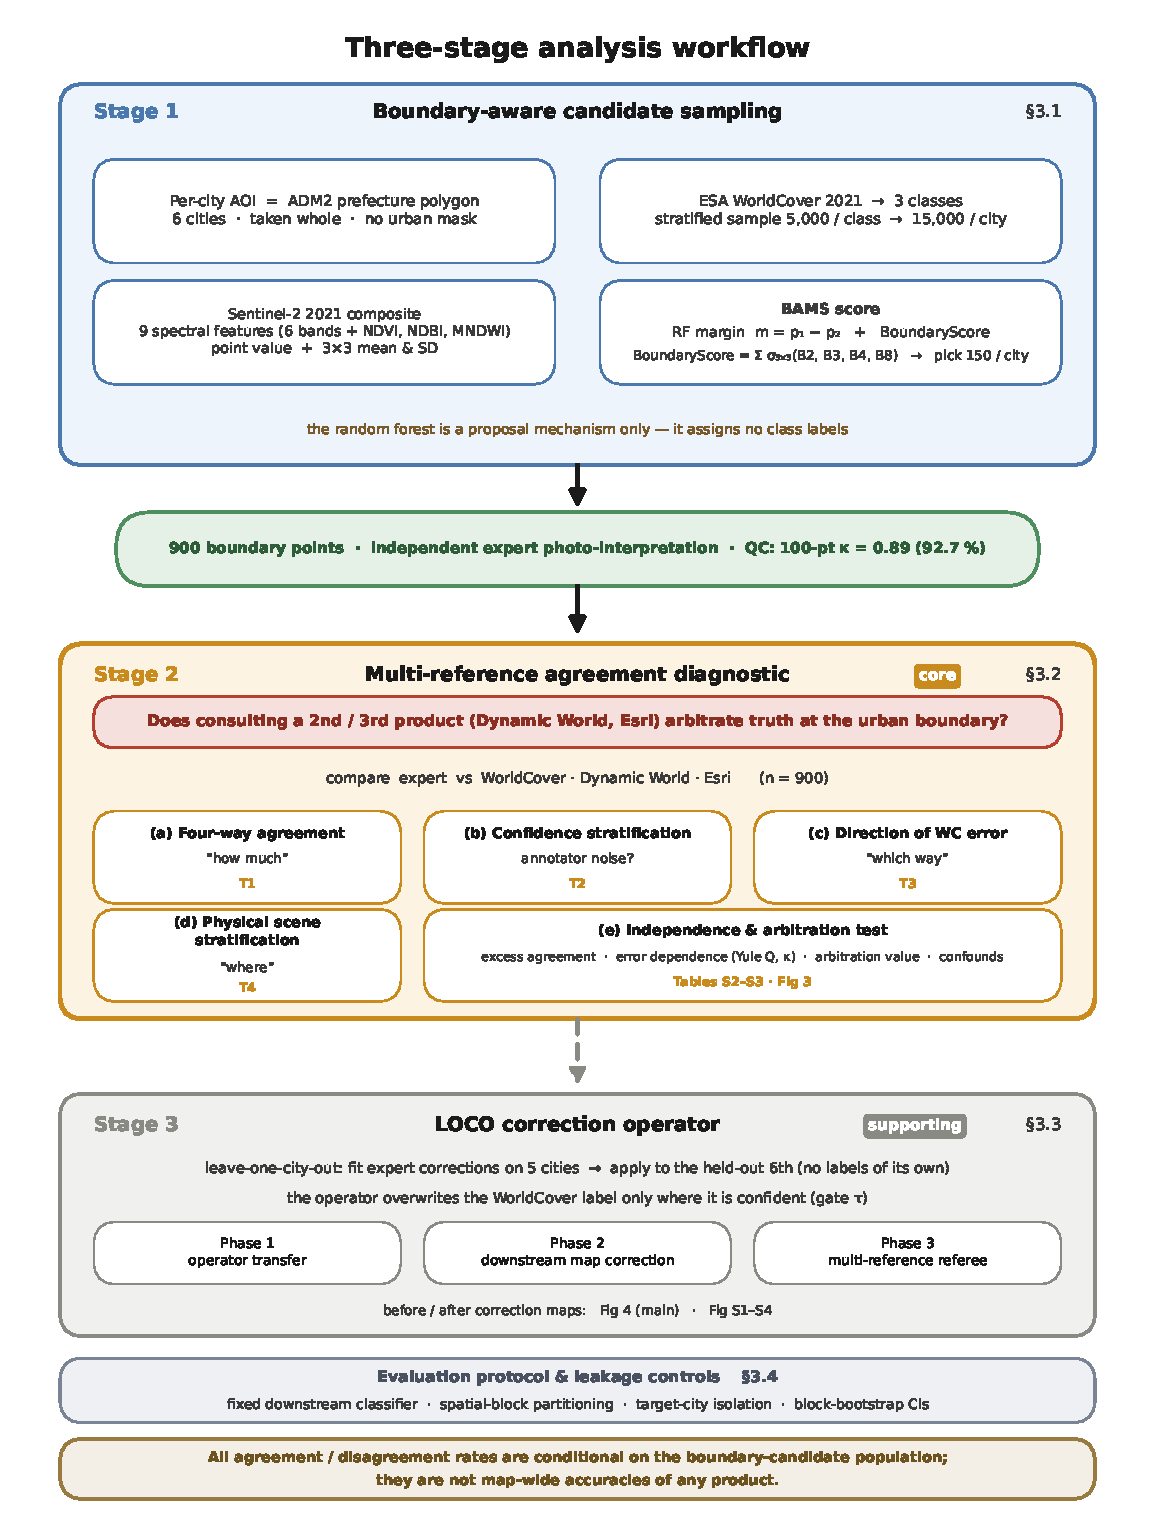
\includegraphics[width=\linewidth]{figures/Figure2_workflow.pdf}
\caption{Analysis workflow. Stage~1: boundary-aware candidate sampling
(Section~\ref{sec:sampling}) $\rightarrow$ 900 expert-labelled points. Stage~2:
the multi-reference agreement diagnostic (Section~\ref{sec:diagnostic}), with
sub-analyses (a)--(e). Stage~3, supporting: the leave-one-city-out correction
operator (Section~\ref{sec:loco}), Phases~1--3.
\label{fig:flowchart}}
\end{figure}

Every agreement and disagreement rate in this paper is computed on the
boundary-candidate points of Section~\ref{sec:sampling}. Because those points
are chosen to be the hardest and most error-prone pixels, the rates are
\textbf{conditional on that population and are not map-wide accuracies} of any
product. The qualifier is not repeated at every number but applies throughout.

\subsection{Boundary-Aware Candidate Sampling}\label{sec:sampling}

\subsubsection*{Candidate pool}

The area of interest for each city is its second-level administrative polygon,
taken whole, with no built-up or urban mask (FAO GAUL 2015, ADM2---the
prefecture-level municipality; \citealp{fao2015gaul}). ESA WorldCover 2021,
v200, at 10~m \citep{zanaga2022} is remapped from its 11 classes to the three
target classes used throughout: \emph{built-up} (WorldCover class 50);
\emph{water} (80 permanent water, 90 herbaceous wetland, 95 mangrove); and
\emph{non-built} (all remaining vegetated and bare classes: 10, 20, 30, 40, 60,
70, 100). Within each polygon we draw a stratified random sample of 5000 points
per remapped class---15,000 points per city (Google Earth Engine
\texttt{stratifiedSample}, 10~m scale, fixed seed)---so the three classes are
balanced before any boundary-aware selection.

The pool spans the whole prefecture rather than a built-up envelope, so it
includes rural land. This is why the scene stratification of
Section~\ref{sec:diagnostic}(d) can report paddy/cropland, forest-edge and
rural-settlement boundary types alongside the urban ones. What concentrates the
900 annotated points onto cover transitions is the boundary-aware step below,
not a spatial mask.

\subsubsection*{Inputs to the sampler}

Feature values come from a single 2021 Sentinel-2 composite, built from
\href{https://developers.google.com/earth-engine/datasets/catalog/COPERNICUS_S2_SR_HARMONIZED}{\path{COPERNICUS/S2_SR_HARMONIZED}} over the full calendar year: scenes with
\path{CLOUDY_PIXEL_PERCENTAGE} $<$ 20 are combined by per-pixel median and
clipped to the administrative polygon. From this composite we take six
surface-reflectance bands (B2, B3, B4, B8, B11, B12) and three spectral indices
(NDVI, NDBI, MNDWI), each as a point value and as a $3 \times 3$ pixel (30~m)
neighbourhood mean and standard deviation. This is the same composite used for
the expert labelling described below. All image processing was carried out in
Google Earth Engine \citep{gorelick2017}.

\subsubsection*{Boundary score}

Boundary-Aware Margin Sampling (BAMS) combines a classifier-uncertainty signal
with a local-heterogeneity signal. The exact procedure is reproduced
deterministically in \path{scripts/reproduce_bams_selection.py}, which
regenerates the on-disk point sets to which the 900 hand labels are anchored
(150/150 match, all six cities).

\begin{enumerate}[leftmargin=*,labelsep=4.5mm]
\item \emph{Classifier margin.} For each city, a random forest (300 trees, fixed
  seed) is fitted on all 15,000 candidates, with the remapped WorldCover label
  as target and the \textbf{nine point-level} spectral features as predictors;
  no neighbourhood terms enter this model. Class posteriors are read back
  in-sample, and the margin of a point is
  %
  \begin{equation}\label{eq:margin}
  m = p_{(1)} - p_{(2)},
  \end{equation}
  %
  the gap between its two largest class posteriors. A small $m$ means the
  spectral signature lies between two classes rather than inside one.
\item \emph{Local spectral heterogeneity.} BoundaryScore is the raw,
  unnormalised sum of the $3 \times 3$ neighbourhood standard deviations of the
  four visible and near-infrared bands,
  %
  \begin{equation}\label{eq:bscore}
  \mathrm{BoundaryScore} = \sigma_{3\times3}(\mathrm{B2}) + \sigma_{3\times3}(\mathrm{B3})
  + \sigma_{3\times3}(\mathrm{B4}) + \sigma_{3\times3}(\mathrm{B8}).
  \end{equation}
  %
  Large values indicate that the 30~m window straddles a cover transition.
\end{enumerate}

This random forest serves only to isolate spectrally ambiguous zones for
annotation; it assigns no class labels. Every boundary candidate was labelled
independently by expert photo-interpretation, so bias in the WorldCover
training targets governs only \emph{which} pixels are examined, not the
reference they are scored against (see ``Sampling-induced conditioning''
below).

\subsubsection*{Selection}

For all six cities, BAMS150 is a two-stage cut: keep the 1000 lowest-margin
points, then keep the 150 of those with the largest BoundaryScore (ascending
\texttt{Original\_ID} is the deterministic final tie-break). A plain
150-smallest-margin set (``Top150'') is generated for reference only and is not
used anywhere downstream.

This places every city's sample deep in the ambiguous regime: per-city median
BAMS150 margin 0.41--0.47, against a full-pool median of $\approx$ 0.95--1.00.
Every diagnostic below is additionally reported per city. Selection yields 150
points per city, 900 in total.

\subsubsection*{Expert labelling}

The 150 points per city were interpreted one by one in the Google Earth Engine
Code Editor at roughly 1:2000 zoom, under a single protocol common to all six
cities. The primary reference was the 2021 Sentinel-2 composite itself, viewed
both as a true-colour rendering (B4/B3/B2, stretched 0--3000) and as a
false-colour infrared rendering (B8/B4/B3, stretched 0--4000). A Google
high-resolution basemap was consulted only as ancillary spatial context---for
form and edge localisation, when the Sentinel-2 view was insufficient. Because
that basemap carries no single acquisition date, the 2021 Sentinel-2 composite
is the temporal anchor of the reference. Each point was assigned the dominant
cover within its 10~m pixel---\{built-up, non-built, water\}---with a
three-level confidence tag (high\,/\,medium\,/\,low) and a free-text scene
note. This produces 900 expert boundary labels, the reference anchor for every
analysis below. The site-selection rationale is given in
Section~\ref{sec:studyarea} and the annotator background in
Section~\ref{sec:annotators}.

Reliability of these single-annotator labels was assessed with an independent
blind re-labelling exercise. Three colleagues at the same centre (A, B and C;
Section~\ref{sec:annotators}), all with operational remote-sensing
image-interpretation experience, each re-labelled a stratified subsample of 120
points (20 per city, proportional to the confidence-tier distribution). They
worked without access to the original labels, the product outputs, or one
another's judgements. Agreement with the reference was almost perfect for all
three (Cohen's $\kappa = 0.95$, 0.91, 0.94; \citealp{landis1977}). Mean
pairwise exact agreement across the six interpreter pairs was 92.67\%, and
multi-rater agreement on the 116 points all three completed was almost perfect
(Fleiss' $\kappa = 0.89$).

\subsubsection*{Sampling-induced conditioning}

BAMS is deliberately non-representative, so the rates in
Section~\ref{sec:results} are conditional on the boundary-candidate population
and are not map-wide product accuracies (Sections~\ref{sec:results-confidence},
\ref{sec:disc-scope}). There is a second source of conditioning: BAMS draws on
Sentinel-2 spectra and Sentinel-2 local heterogeneity, while the expert
reference is read chiefly from a 2021 Sentinel-2 composite, so selection and
reference share a common information base. This is examined in
Section~\ref{sec:disc-scope}.

\subsection{Multi-Reference Agreement Diagnostic}\label{sec:diagnostic}

\subsubsection*{Reference layers}

Three global 10~m products are compared with the expert labels. ESA WorldCover
2021 v200 (WC) is a gradient-boosted-tree classifier with a rule-based
post-process on Sentinel-1/2 \citep{zanaga2022}. Dynamic World (DW) is a
fully-convolutional semantic-segmentation model that produces
near-instantaneous per-scene Sentinel-2 predictions; we take the 2021 annual
label mode \citep{brown2022}. Esri Land Cover (Esri\,/\,Impact Observatory) is
a deep segmentation model run on annual Sentinel-2 composites \citep{karra2021}.

Each product is sampled at the 900 boundary points and remapped to the same
three classes (Table~\ref{tab:legend_map}). WC, DW and Esri are available for
all six cities (multi-reference subset $n = 900$). Every WorldCover quantity
uses the stored 2021 v200 class; an independently re-sampled WorldCover layer is
kept only as a cross-check and enters no reported number. Binomial proportions
are reported with Wilson 95\% confidence intervals \citep{wilson1927}.

The diagnostic has five parts.

\paragraph{(a) Four-way agreement (Table~\ref{tab:T1}).}
We compute pairwise agreement rates among \{expert, WC, DW, Esri\}, plus the
tri-agreement fraction (expert $=$ DW $=$ Esri) and the four-way agreement
fraction, pooled ($n = 900$) and per city.

\paragraph{(b) Confidence stratification (Table~\ref{tab:T2}).}
The expert $\neq$ WC disagreement rate is computed over all labels, over the
high\,+\,medium subset, and over the high-confidence-only subset, per city and
pooled. This tests whether the disagreement is merely annotator noise on
ambiguous pixels: if it were, it should shrink on the high-confidence subset.
The test has a built-in bias---an annotator may assign ``high'' precisely when
a WC error is obvious---which we take into account when reading the result
(Section~\ref{sec:results-confidence}, Section~\ref{sec:disc-scope}).

\paragraph{(c) Direction of the WC error (Table~\ref{tab:T3}).}
From the WC $\to$ expert confusion matrix on the boundary points we report the
conditional error rates $P(\text{expert} = \text{non-built} \mid \text{WC} =
\text{built})$ and $P(\text{expert} = \text{built} \mid \text{WC} =
\text{non-built})$, and the net over-\,/\,under-call of built-up,
%
\begin{equation}\label{eq:netbuilt}
\Delta_{\text{built}} = \frac{n(\text{expert} = \text{non-built} \mid \text{WC} = \text{built})
- n(\text{expert} = \text{built} \mid \text{WC} = \text{non-built})}{n}.
\end{equation}

\paragraph{(d) Physical scene stratification (Table~\ref{tab:T4}).}
Each boundary point carries a free-text scene note recorded during annotation.
Using the annotator-supplied scene-code table, we grouped these notes into
physical boundary types (built-up edge\,/\,urban fabric; urban green space;
road\,/\,road edge; water\,/\,water edge; vegetation\,/\,forest edge;
paddy\,/\,cropland; rural settlement; bare land\,/\,construction), and we report
the expert $\neq$ WC disagreement rate, with Wilson intervals, for groups with
$n \ge 15$. This is a keyword-based localisation aid, not a formal stratified
sample (Section~\ref{sec:disc-scope}). The scene notes are free-text, so
scene-type contrasts are drawn only in the pooled set. The grouping covers the
891 boundary points whose note resolves to a single physical boundary type; the
remaining nine carried no resolvable type and are omitted. The 26 Nanchang
points initially recorded without a scene note---their expert class
placeholder-filled from WorldCover during annotation---were re-annotated on
sub-metre imagery by two annotators and assigned an expert class and a scene
code; 13 of the 26 disagree with WorldCover.

\paragraph{(e) Independence and arbitration test (Section~\ref{sec:results-independence};
Table~\ref{tab:S2}, Figure~\ref{fig:independence}).}
Multi-reference arbitration implicitly assumes the references approach the truth
\emph{independently}, so that agreement between two of them corroborates a
label. We test that assumption on the $n = 900$ subset, using the expert label
$H$ as the best available stand-in for the true class throughout. All three
checks below are therefore statements about dependence relative to the current
expert reference, not about an unconditional ground truth. (S2c) scores a
prediction directly against $H$ itself; (S2a) conditions the comparison
between products on $H$'s class labels, and (S2b) defines each product's
error relative to $H$ before comparing those errors. All three remain
dependent on $H$'s reliability; we do not have a reference-noise model
precise enough to rank how tightly each depends on it
(Section~\ref{sec:disc-scope}).
\emph{(S2a) Excess agreement:} observed pairwise agreement is compared with the
value expected if the two products $A$ and $B$ were conditionally independent
given the true class $Y$, taken operationally as $H$,
%
\begin{equation}\label{eq:condindep}
P_{\text{indep}}(A = B) = \sum_{j} P(H = j) \sum_{c} P(A = c \mid H = j)\,P(B = c \mid H = j).
\end{equation}
%
The conditional class distributions are estimated from the same sample used to
compute the observed agreement, stratified by the expert-label class $j$
(stratum sizes $n_j = 231, 516, 153$); under within-stratum i.i.d.\ sampling,
same-sample self-pairing shrinks the \emph{expected excess} (observed minus
independence-implied agreement) toward zero within each stratum by a factor
of $(1-1/n_j)$ relative to its population value; equivalently, the plug-in
null is biased by $\Delta_j/n_j$ per stratum, where $\Delta_j$ is that
stratum's population excess (upward when $\Delta_j > 0$, as here). Recomputing the DW/Esri
excess with this stratum-wise finite-sample correction moves it from 0.2577
to 0.2584---an increase of less than 0.001, too small at this sample size to treat the
raw plug-in value as materially conservative. Uncertainty is a 4000-sample point bootstrap with a
leave-one-city-out range. \emph{(S2b) Error dependence:} with $e_{A} =
\mathbf{1}\{A \neq \text{expert}\}$ we compute Yule's $Q$ \citep{yule1900},
Cohen's $\kappa$ and the co-error ratio between each pair of product error
indicators; like (S2a), this is the joint error structure of the three
products relative to $H$, not an unconditional statement about the products'
own errors. \emph{(S2c) Arbitration value:} we evaluate $P(\text{expert} = \ell \mid
\text{DW} = \text{Esri} = \ell)$ against the single-product baselines
$P(\text{expert} = \text{DW})$ and $P(\text{expert} = \text{Esri})$ and against
the WC\,$=$\,DW consensus. \emph{(S3) Confound checks:} the ontology is
collapsed to two classes (built vs.\ rest, and built-vs-non-built with water
points dropped) and the test repeated; WorldCover serves as a negative control
(same Sentinel-2 input, different model family); and the DW\,$=$\,Esri
agreement rate is resolved by scene type. The ontology and by-scene tables are
in the Supplementary Material (Tables~S3, S4).

\subsection{LOCO Correction Operator (Supporting Analysis)}\label{sec:loco}

We first tried propagating the boundary labels to their spectral neighbours
\emph{within the same city}---our variant of the prototype\,/\,pseudo-label
rectification-and-expansion family, of which PRE \citep{tong2024pre} is a
representative instance (\emph{Prototype Expansion}). It leaks under spatial
autocorrelation: once evaluation points are excluded from the neighbour
search, the procedure produces no valid expansions, and the apparent gain it
showed without that control traces to a classifier change, not to propagation
(full leakage diagnostic in Supplementary S5). We instead define a correction
operator trained on the labelled points of $N - 1$ cities and transferred to a
held-out city that contributes no labels of its own---leave-one-city-out
(LOCO)---which removes this dependence by construction, and report it as a
supporting result, not the paper's main claim.

\subsubsection*{Operator}

For a held-out city $c$, a random forest (300 trees) is trained on the pooled
150-point boundary sets of the other five cities. The input is a 27-feature
vector---the nine point-level spectral features plus their nine $3 \times 3$
neighbourhood means and nine $3 \times 3$ neighbourhood standard
deviations---the target is the expert class, and samples are weighted by
confidence tier (high 1.0, medium 0.6, low 0.3). Applied to city $c$'s 150
boundary points, it returns a predicted class and its posterior $p_{\max}$ for
each point. The operator \emph{fires}---overwrites the WorldCover label---only
where it is both confident and dissenting: $p_{\max} \ge \tau$ ($\tau = 0.85$)
and predicted class $\neq$ WC class. For the downstream-map experiment
(Phase~2), a boundary gate further restricts firing: only candidates in the
lowest decile of within-city margin are eligible. A reduced-feature variant is
reported in Supplementary S2.

\subsubsection*{Phase 1---operator transfer}

The LOCO operator is applied to the held-out city's 150 boundary points, and
its predicted class is scored against the expert label, relative to the ``do
nothing'' baseline (the WC $=$ expert rate). We report operator accuracy, the
number of confident firings, and their precision against the expert label.

\subsubsection*{Phase 2---downstream classifier training}

Every baseline and corrected variant in this phase is scored with the same
downstream classifier---a random forest, 300 trees, scikit-learn defaults
otherwise---so no change of classifier architecture can be mistaken for a
method effect. For each held-out city and each of five spatial-block
partition seeds, this classifier is trained on the city's $\approx$ 10,000
non-boundary training points; splits are made by whole spatial cells, not by
random points (each city gridded into $6 \times 6$ cells on
latitude/longitude quantiles, whole cells assigned to the test set until
$\approx$ 30\% of points are held out), so training and test points are drawn
from disjoint spatial blocks, which reduces but---at block edges, given the
$3 \times 3$ neighbourhood features---does not fully eliminate the chance of
near-duplicate neighbours across the split. This spatial-block split governs
the $\approx$ 10,000-point WorldCover training/test pool only; the 150
expert points are excluded from training in every case, but are not
themselves partitioned by the same split, so some sit geographically inside
the training block (checked in Section~\ref{sec:results-loco}). Five
labelling schemes are compared: (B0)~raw WC labels; (B2)~WC labels corrected by the transferred LOCO
operator on boundary-gated, confidence-gated points---\emph{the proposed
method}; (B1)~a \emph{within-city oracle} operator that does see city $c$'s
expert labels (an optimistic ceiling rather than a mathematical upper bound,
since it is itself an estimated model, not a guarantee); (B3)~the transferred
operator without the
boundary gate (ablation); and (B4)~the same number of labels, drawn from the
same gated candidate pool as B2, flipped to a uniformly random one of the
other two classes (control, using the same five spatial-block seeds); a flip
only has a chance of landing on the correct class when the original
WorldCover label was itself wrong, so its expected success rate is not a
fixed one-third baseline. The correction operator never sees the held-out city,
and the downstream classifier never sees the held-out city's expert
labels---its 150 boundary points are evaluation-only. Each classifier is
scored for overall accuracy (OA) and Boundary Error (BE), defined as the
number of built $\leftrightarrow$ non-built confusions,
%
\begin{equation}\label{eq:be}
\mathrm{BE} = cm[\text{built}, \text{non-built}] + cm[\text{non-built}, \text{built}],
\end{equation}
%
on the held-out spatial-block test set (against WC) and, separately, on the
full set of 150 expert points, which are never used for training but are not
restricted to the test block (against the expert). A $\tau \times$
margin-quantile sensitivity sweep is in Supplementary Table~S1.

\subsubsection*{Phase 3---multi-reference referee}

The corrected label map is evaluated directly, with no downstream classifier,
on the 150 held-out points of each city,
against (i)~the expert label and (ii)~the strict tri-consensus subset expert
$=$ DW $=$ Esri. Of the points the operator changed, we report the fraction
moved toward the expert label and the fraction moved toward the DW/Esri
consensus, with the random-flip control and the within-city oracle ceiling for
reference.

\subsubsection*{Reproducibility}

All inputs, analysis scripts and frozen result snapshots are listed in the Data
Availability statement. BAMS point selection is regenerated by
\path{scripts/reproduce_bams_selection.py}. The pipeline runs in a fixed
conda environment with a scikit-learn RandomForest throughout (no GPU or
neural-network components).

%% ===================== 4  RESULTS ===============================
%% =====================================================================
%%  body/results.tex  --  Section 4 (Results)
%%  Drop-in fragment; compiles only inside the MDPI Remote Sensing template.
%%
%%  2026-09-10 — readability pass (sentence-level only). Split long
%%  multi-clause sentences; broke one garden-path ("disagrees as often as
%%  the built-up edge is consistent with ...") into two sentences with the
%%  same meaning.
%%
%%  2026-09-10 (2) — ALL NUMBERS REFRESHED for the Hangzhou two-stage
%%  standardisation (see body/methods.tex header and
%%  data/analysis_outputs/hangzhou_standardise/RESULTS_before_after.md).
%%  Only Hangzhou's 150 points changed; the other five cities are identical.
%%  Qualitative changes: (1) WorldCover-pair error coupling now weakly
%%  positive (Yule's Q ~ 0.08 / 0.14) not ~0 — "Q ~ 0 for WC pairs" wording
%%  replaced by "Q <= 0.14 vs 0.97"; (2) LOCO (supporting) got more
%%  conservative — fewer downstream firings, same "within between-seed
%%  noise" conclusion. S5 operator-transfer data below also updated.
%%
%%  2026-09-10 (3) — SCENE STRATIFICATION now six-city. Hangzhou folded into
%%  T4 / S3c (scripts/hangzhou_scene_rows.py; its 43 veg-edge points split
%%  urban-green/forest-edge from imagery, scripts/gee_hangzhou_veg_subclass.js).
%%  T4 pooled over the 891 points with a resolvable scene note (was "five-city
%%  n=750"); "Hangzhou has no scene-code table" / "five-city" call-outs
%%  removed; the per-city "short codes vs Chinese free text" line dropped.
%%  Urban green space is now the single highest group (67.3%) vs built-up edge
%%  66.1% (was tied at 69.0%). New row: Cropland / paddy transition n=16.
%%  S6 per-city counts below also updated for the two-stage maps.
%%
%%  2026-09-11 — external-review fix pass (Remote_Sensing_投稿评估.md):
%%  (1) Table T3 paragraph said "the expert reads vegetation" for the WC
%%  built -> expert non-built rate, but T3's "non-built" is a merged class
%%  (vegetation + bare soil + other); reworded to "the expert reads
%%  non-built" -- no numbers changed. (2) Confound-checks paragraph
%%  (sec:results-independence) asserted as fact that WorldCover "shares
%%  neither the deep-segmentation model family nor its point-label lineage"
%%  with DW/Esri -- the point-label-lineage half contradicted the Discussion
%%  (sec:disc-mechanism), which correctly treats shared training-label
%%  lineage as an undocumented, untestable possibility. Reworded to state
%%  only the model-family contrast, which is citable (zanaga2022 vs
%%  brown2022/karra2021). (3) Arbitration-value exception to "central
%%  contrast does not require the expert label to be ground truth" now
%%  flagged inline; "conservative lower bound" reworded to "expected to
%%  understate the true value" (see body/methods.tex header for the source
%%  of both).
%%
%%  2026-09-14 — bams150_scene_grouped.csv carried Changsha (36 pts) and
%%  Wuhan (7 pts) Human_Class from a pre-correction snapshot (matching
%%  *_BAMS150_Manual_bk.csv) instead of the current 04_manual labels;
%%  scripts/fix_scene_csv_changsha_wuhan.py corrected it and T4 was
%%  regenerated. Urban green space rises 67.3% -> 71.2% and is now clearly
%%  the single highest group (previously near-tied with built-up edge);
%%  built-up edge falls 66.1% -> 62.6%, moving behind road/road edge (62.4%
%%  -> 64.1%); water/bare-land/vegetation-forest-edge shift by 1-2 points;
%%  rural settlement / paddy / cropland-transition / mixed are untouched (no
%%  Changsha or Wuhan points in those groups). No other table in the paper
%%  (T1-T3, T5, S2a-c, S3a-c) reads from this file's Human_Class column, so
%%  none of them changed -- confirmed by diffing against docs/results_snapshot.
%%
%%  Cite keys: yuan2026
%%  Labels defined: sec:results sec:results-agreement sec:results-confidence
%%                  sec:results-errordir sec:results-scene
%%                  sec:results-independence sec:results-loco
%%                  tab:T1 tab:T2 tab:T3 tab:T4 tab:S2 tab:phase3
%%  Labels expected: fig:independence fig:map_maintext tab:S1
%%                   sec:sampling sec:diagnostic sec:loco
%%                   sec:disc-edge sec:disc-mechanism sec:disc-loco
%%                   sec:disc-scope app:recheck
%%                   eq:netbuilt eq:be
%%
%%  SUPPLEMENTARY tables/figures referenced by this section, all now in
%%  docs/manuscript_supplementary.md:
%%   S3  ontology confound            (existing)
%%   S4  by-scene DW=Esri rate        (existing, table lives in supp. S3)
%%   S5  LOCO operator transfer, per city            -- added 2026-09-11, supp. S4
%%   S6  per-city operator-change / expert!=WC counts -- added 2026-09-11, supp. S4
%%   Figures S1-S4  before/after maps, Wuhan/Hefei/Nanchang/Hangzhou
%%                                                    -- added 2026-09-11, supp. S4
%% =====================================================================

\section{Results}\label{sec:results}

All rates below are computed on the 900 boundary-candidate points of
Section~\ref{sec:sampling} and are \textbf{conditional rates on that
population, not map-wide accuracies} of ESA WorldCover, Dynamic World or Esri
Land Cover. Sections~\ref{sec:results-agreement}--\ref{sec:results-independence}
report the multi-reference diagnostic---how much the three products depart from
the expert labels, whether that departure is annotator noise, which direction
the WorldCover error runs, which physical boundary types it concentrates in,
and whether a second and third product supply independent corroboration.
Section~\ref{sec:results-loco} reports the supporting LOCO correction
operator, including the before/after maps. Class codes are
1~$=$~built-up, 2~$=$~non-built, 3~$=$~water.

\subsection{Multi-Reference Agreement at the Boundary}\label{sec:results-agreement}

Table~\ref{tab:T1} gives the pairwise agreement rates among \{expert, WC, DW,
Esri\} on the boundary candidates, pooled ($n = 900$) and per city.

\begin{table}[H]
\caption{Four-way agreement on the boundary candidates. ``H'' $=$ expert label.
Pooled expert $=$ WC is 0.47, Wilson 95\% CI [0.43, 0.50]. Per-city $n = 150$.\label{tab:T1}}
\begin{adjustwidth}{-\extralength}{0cm}
\footnotesize
\begin{tabularx}{\fulllength}{lCCCCCCCCC}
\toprule
\textbf{City} & \textbf{\textit{n}} & \textbf{H\,$=$\,WC} & \textbf{H\,$=$\,DW}
& \textbf{H\,$=$\,Esri} & \textbf{WC\,$=$\,DW} & \textbf{WC\,$=$\,Esri}
& \textbf{DW\,$=$\,Esri} & \textbf{H\,$=$\,DW\,$=$\,Esri} & \textbf{All four}\\
\midrule
Wuhan     & 150 & 0.41 & 0.51 & 0.50 & 0.47 & 0.45 & 0.91 & 0.47 & 0.19\\
Hefei     & 150 & 0.51 & 0.39 & 0.41 & 0.49 & 0.53 & 0.83 & 0.33 & 0.17\\
Nanchang  & 150 & 0.46 & 0.39 & 0.36 & 0.36 & 0.45 & 0.81 & 0.29 & 0.11\\
Nanjing   & 150 & 0.32 & 0.43 & 0.43 & 0.47 & 0.47 & 0.93 & 0.40 & 0.11\\
Changsha  & 150 & 0.51 & 0.43 & 0.35 & 0.49 & 0.47 & 0.87 & 0.33 & 0.18\\
Hangzhou  & 150 & 0.59 & 0.53 & 0.48 & 0.63 & 0.60 & 0.90 & 0.46 & 0.34\\
\midrule
\textbf{Pooled} & \textbf{900} & \textbf{0.47} & \textbf{0.45} & \textbf{0.42}
& \textbf{0.48} & \textbf{0.50} & \textbf{0.87} & \textbf{0.38} & \textbf{0.18}\\
\bottomrule
\end{tabularx}
\end{adjustwidth}
\end{table}

The one rate that is high everywhere is DW $=$ Esri: 0.81 to 0.93 across all
six cities, pooled 0.87---against an expert $=$ DW of only 0.45. The two
products that agree closely with each other do not agree with the expert, and
neither does the third: pooled, expert $=$ WC is 0.47 [0.43, 0.50], expert $=$
DW 0.45, expert $=$ Esri 0.42. Substituting one product for another does not
help---the cross-product rates WC $=$ DW (0.48) and WC $=$ Esri (0.50) sit
barely above the product-versus-expert rates and nowhere near a level that
would resolve the boundary. The four sources coincide unanimously on only 18\%
of boundary candidates. On the remaining $\approx$ 82\% at least one dissents.
A two-product majority is not scarce---DW and Esri alone agree on 87\% of
points---but that majority is joined by the expert label on only 38\% of the
900 points (the largest internally consistent subset, expert included).
Consulting a second and a third global product therefore does not arbitrate
land-cover class boundaries: a product majority exists almost everywhere, but requiring
it does not raise the aggregate agreement with the expert label above what a
single product achieves alone.

The per-city expert $=$ WC rate ranges from 0.32 (Nanjing, the lowest) to 0.59
(Hangzhou); the full set is in Table~\ref{tab:T1}. Whether the DW $=$ Esri
agreement is independent corroboration---and therefore usable for
arbitration---is tested directly in Section~\ref{sec:results-independence}.

\subsection{Confidence Stratification}\label{sec:results-confidence}

If the expert--WC disagreement were annotator noise on inherently ambiguous
pixels, it should shrink when the analysis is restricted to the labels the
annotator marked ``high'' confidence. Table~\ref{tab:T2} shows the opposite.

\begin{table}[H]
\caption{Expert $\neq$ WC disagreement rate by expert confidence tier. Pooled
high-only rate 0.67, Wilson 95\% CI [0.62, 0.71].\label{tab:T2}}
\begin{adjustwidth}{-\extralength}{0cm}
\small
\begin{tabularx}{\fulllength}{lCCCCCCC}
\toprule
\textbf{Stratum} & \textbf{Pooled} & \textbf{Wuhan} & \textbf{Hefei}
& \textbf{Nanchang} & \textbf{Nanjing} & \textbf{Changsha} & \textbf{Hangzhou}\\
\midrule
All labels     & 0.53 ($n = 900$) & 0.59 & 0.49 & 0.54 & 0.68 & 0.49 & 0.41\\
High\,+\,medium & 0.55 ($n = 813$) & 0.58 & 0.49 & 0.54 & 0.68 & 0.57 & 0.42\\
High only      & \textbf{0.67 ($n = 419$)} & 0.88 & 0.53 & 1.00 ($n = 42$) & 0.62 & 0.58 & 0.55\\
\bottomrule
\end{tabularx}
\end{adjustwidth}
\end{table}

The pooled expert $\neq$ WC rate rises from 0.53 over all labels to 0.67
[0.62, 0.71] on the high-confidence subset. The rise holds in five of six
cities and is steep in two: Wuhan 0.59 $\to$ 0.88, and Nanchang, where all 42
high-confidence boundary labels disagree with WorldCover. Nanjing is the sole
exception, easing from 0.68 to 0.62, and it starts from the highest all-label
rate of the six. Where the expert is most certain, WorldCover is not closer to
the expert but further from it.

Disagreement remains high among labels marked as high confidence. However,
annotators may assign high confidence when a product error is visually
obvious, so confidence selection may contribute to this pattern. The blind
re-check below provides additional evidence of product error.

A targeted check addresses the same concern from the other side. From the
high-confidence expert $\neq$ WorldCover subset (281 points; Appendix~\ref{app:recheck}
records the pre-relabelling count), we drew 30---five per city, in decreasing
BAMS classifier margin. An
analyst who had taken no part in the original labelling re-classified them
from sub-metre satellite imagery and the 2021 Sentinel-2 composite, blind to
both the expert label and the WorldCover label (Appendix~\ref{app:recheck}).
The re-classification reproduced the original expert label on 29 of the 30
points and matched the WorldCover label on none; the one exception was a mixed
water/vegetation edge pixel the second analyst could not resolve. This removes
the same-analyst circularity in reading these disagreements as WorldCover
error. It is not a fully independent measurement, though: the second analyst
shared the imagery sources, so this is an independent judgement, not a fully
independent measurement.

\subsection{Direction of the WorldCover Error}\label{sec:results-errordir}

Table~\ref{tab:T3} is the pooled WC $\to$ expert confusion matrix on the 900
boundary points.

\begin{table}[H]
\caption{WC $\to$ expert confusion on the boundary candidates (counts), six
cities pooled. Rows are the WorldCover class, columns the expert class.\label{tab:T3}}
\begin{tabularx}{\textwidth}{lCCCC}
\toprule
\textbf{WC label} & \textbf{expert $=$ built} & \textbf{expert $=$ non-built}
& \textbf{expert $=$ water} & \textbf{row \textit{n}}\\
\midrule
WC $=$ built     & 72  & 197 & 10 & 279\\
WC $=$ non-built & 152 & 262 & 57 & 471\\
WC $=$ water     & 7   & 57  & 86 & 150\\
\bottomrule
\end{tabularx}
\end{table}

Derived from the matrix: $P(\text{expert} = \text{non-built} \mid \text{WC} =
\text{built}) = 0.71$, $P(\text{expert} = \text{built} \mid \text{WC} =
\text{non-built}) = 0.32$, and the net over-call of built-up
(Equation~\eqref{eq:netbuilt}), $\Delta_{\text{built}} = (197 - 152)/900 =
45/900 = 0.05$. In aggregate the boundary error is close to
symmetric---WorldCover is not simply over- or under-painting built-up along the
edge---but it is conditionally asymmetric: once WorldCover commits to
``built-up'' at a boundary candidate, roughly seven times in ten the expert
reads non-built. The non-built\,$\mid$\,built rate is between 0.60 and 0.79 in
every one of the six cities. This one-directional signal---a WC ``built-up''
call at the boundary is untrustworthy in a specific, predictable way---is what
the correction operator of Section~\ref{sec:results-loco} exploits. Figure~S5
in the Supplementary Material shows example Sentinel-2 chips illustrating this
directional pattern; the quantitative claim rests on Table~\ref{tab:T3} above,
not on the gallery.

This directional error bears directly on the practice of treating
cross-product agreement as a pseudo-label. Restricting to the points where DW
and Esri agree, the retained sample's own expert-label composition
stays close to the full 150-point sample in each city (non-built by the
expert: 51--64\% retained vs.\ 53--65\% in the full sample; pooled 56.2\% vs.\
57.3\%)---but taking the class agreed upon by Dynamic World and Esri as a
pseudo-label assigns only 2--8\% of those same points to non-built. Using the
agreed product class as a pseudo-label under-represents non-built cover among
the retained points; the bias is in the label given to the retained points,
not in which points the filter happens to keep.

\subsection{Physical Scene Stratification}\label{sec:results-scene}

Each boundary point carries a free-text scene note recorded during annotation
(Section~\ref{sec:diagnostic}(d)). Notes were grouped into physical boundary
types using the annotator's scene-code table, and the expert $\neq$ WC rate
computed per group for groups with $n \ge 15$. The grouping covers the 891
boundary points whose note resolves to a single boundary type (all 900 less
nine), and includes the 26 Nanchang points that were re-annotated from imagery
after an annotation placeholder was found (Section~\ref{sec:diagnostic}(d)).

\begin{table}[H]
\caption{Expert $\neq$ WC disagreement by physical boundary type, pooled over
the 891 boundary points with a resolvable scene note, groups with
$n \ge 15$.\label{tab:T4}}
\begin{tabularx}{\textwidth}{lCCC}
\toprule
\textbf{Scene group} & \textbf{\textit{n}} & \textbf{\mbox{Expert $\neq$ WC}}
& \textbf{Wilson 95\% CI}\\
\midrule
Urban green space              & 52  & 71.2\% & [58, 82]\\
Road / road edge               & 117 & 64.1\% & [55, 72]\\
Built-up edge / urban fabric   & 174 & 62.6\% & [55, 69]\\
Vegetation / forest edge       & 130 & 53.1\% & [45, 61]\\
Water / water edge             & 211 & 48.3\% & [42, 55]\\
Bare land / construction       & 88  & 44.3\% & [34, 55]\\
Rural settlement / surfaces    & 41  & 41.5\% & [28, 57]\\
Paddy / cropland / field       & 19  & 36.8\% & [19, 59]\\
Cropland / paddy transition    & 16  & 31.2\% & [14, 56]\\
Mixed / complex                & 25  & 28.0\% & [14, 48]\\
\bottomrule
\end{tabularx}
\end{table}

Disagreement is highest exactly where built-up meets vegetation. Urban green
space is the single highest group (71.2\%), ahead of road / road edge
(64.1\%) and the built-up edge itself (62.6\%), all well above bare land /
construction (44.3\%) and rural settlement (41.5\%),
where the cover classes are more spectrally separable. Urban green space---parks,
street trees, campus and residential greenery embedded in the built
matrix---disagrees even more than the built-up edge itself does. That is consistent with
the documented
tendency of global products to absorb intra-urban vegetation into the built
class (Section~\ref{sec:disc-edge};~\citealp{yuan2026}), and we report it here
as a finding in its own right, not only a category in the table. The grouping
locates the disagreement rather than estimating a population quantity; its
caveats are in Section~\ref{sec:diagnostic}(d) and Section~\ref{sec:disc-scope}.

\subsection{Independence and Arbitration}\label{sec:results-independence}

Multi-reference arbitration assumes the references approach the truth
\emph{independently}, so that agreement between two of them corroborates a
label. Section~\ref{sec:results-agreement} showed DW and Esri agreeing with
each other far more (0.87) than either agrees with the expert ($\approx$ 0.43).
This section tests whether that mutual agreement is independent corroboration.
All statistics are on the $n = 900$ subset, using the expert label $H$ as the
best available stand-in for the true class throughout. Excess agreement and
error dependence, below, are therefore statements about dependence relative
to $H$, not about an unconditional ground truth. The arbitration-value check
is bound most directly by $H$'s own reliability, since it evaluates
prediction directly against the expert reference
(Section~\ref{sec:diagnostic}(e)). Figure~\ref{fig:independence}
summarises.

\begin{figure}[H]
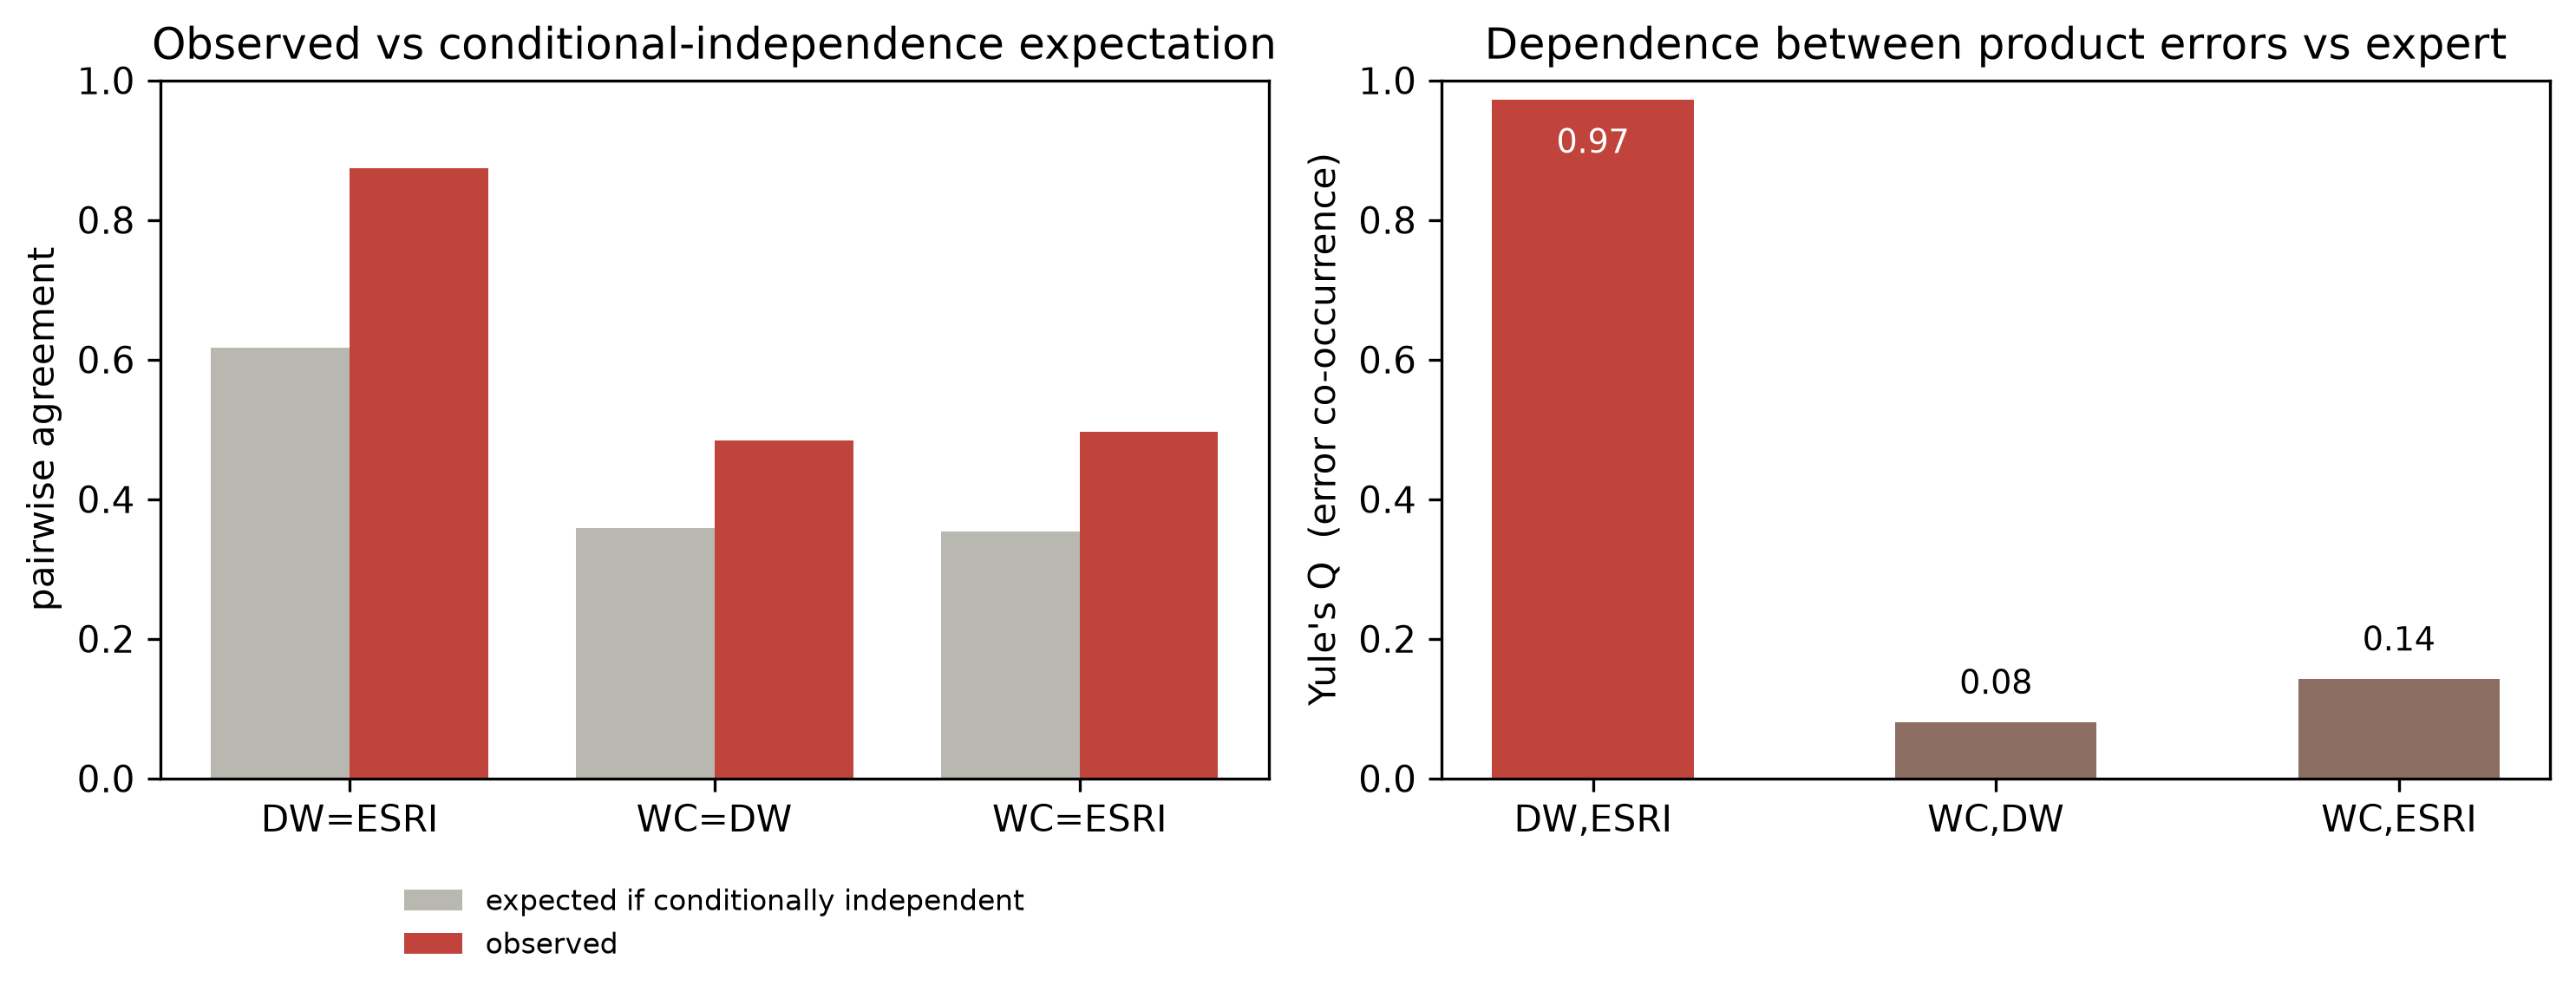
\includegraphics[width=\linewidth]{figures/Figure3_independence.png}
\caption{Conditional-independence diagnostic for the product error indicators
$e_A = \mathbf{1}\{A \neq \text{expert}\}$ on the $n = 900$ boundary subset:
observed pairwise agreement against the value expected under conditional
independence (left), and Yule's $Q$ between each pair of product error
indicators (right); Cohen's $\kappa$ between the same error pairs (S2b) is
reported alongside Yule's $Q$ in Table~\ref{tab:S2}.
\label{fig:independence}}
\end{figure}

\paragraph{Excess agreement.}
DW and Esri agree 0.26 more often than conditional independence allows
(observed 0.87 against an expected 0.62; bootstrap 95\% CI on the excess
[0.23, 0.29], leave-one-city-out range [0.24, 0.27])---about twice the excess
of either WorldCover pair ($+$0.13 for WC $=$ DW, $+$0.14 for WC $=$ Esri).
A finite-sample correction for the same-sample self-pairing in this estimate
(derived in Section~\ref{sec:diagnostic}(e)) moves the precise DW/Esri value
from 0.2577 to 0.2584---both rounding to the reported $+$0.26, an increase of
less than 0.001, too small to matter at the reported precision.

\paragraph{Error dependence (Table~\ref{tab:S2}).}
This is the sharpest result of the diagnostic. With $e_A = \mathbf{1}\{A \neq
\text{expert}\}$, DW and Esri err on 55\% and 58\% of boundary candidates and
co-err on 51\%, against 32\% expected if their errors were independent. Yule's
$Q$ between their error indicators is 0.97 [0.96, 0.98], and when both err they
select the same wrong class 97\% of the time. For the WorldCover pairs $Q$ is an
order of magnitude smaller---$+$0.08 [$-$0.05, 0.21] for WC, DW and $+$0.14
[0.01, 0.27] for WC, Esri, against 0.97, with $\kappa$(errors) of 0.04 and 0.07
against 0.78. The point-level bootstrap treats the 900 points as i.i.d., but
the sample is a fixed 150-point block per city, so we also report a
city-block bootstrap (resampling the six cities, not the points, with
replacement). Under that wider interval the DW/Esri coupling is still clearly
bounded away from zero ([0.95, 0.99]), while both WorldCover pairs widen to
include zero (WC, DW [$-$0.14, 0.32]; WC, Esri [$-$0.01, 0.33])---so only the
DW/Esri error coupling is robust to city-level clustering; the small
WorldCover-pair point estimates are not distinguishable from zero once that
clustering is accounted for. WorldCover's errors are at most
weakly coupled to the two deep-segmentation products; those two err together.
This is a large, asymmetric differential between the product pairs rather than
a shift shared uniformly across all three. We do not have a reference-noise
model precise enough to say what pattern a shared expert-labelling bias would
itself produce, so this asymmetry does not by itself rule out an
expert-dependent explanation---an expert error that happens to align
specifically with WorldCover's own error mode could still leave the
WorldCover pairs looking artificially less coupled; the blind re-classification
check (Section~\ref{sec:disc-scope}) bears on this possibility more directly. (The ``same wrong class'' rate is $\approx$ 0.87 for
the WorldCover pairs too, because with three classes two products that both err
on a boundary point usually land in the same
built\,$\leftrightarrow$\,non-built confusion; the pairs are separated by $Q$
and $\kappa$, not by this rate.)

\begin{table}[H]
\caption{Dependence of the product error indicators $e_A = \mathbf{1}\{A \neq
\text{expert}\}$ on the $n = 900$ boundary subset: observed co-error rate
against the marginal-independent value, Yule's $Q$ (point-level and
city-block bootstrap 95\% CIs) and Cohen's $\kappa$. Excess
pairwise agreement (S2a) and arbitration value (S2c) are reported in the text;
the diagnostic is summarised in Figure~\ref{fig:independence}.\label{tab:S2}}
\begin{adjustwidth}{-\extralength}{0cm}
\small
\begin{tabularx}{\fulllength}{lCCCCCC}
\toprule
\textbf{Error pair} & \textbf{Error rate A / B}
& \textbf{Co-error obs / indep (ratio)} & \textbf{Yule's \textit{Q} [point-bootstrap 95\% CI]}
& \textbf{[city-block 95\% CI]}
& \textbf{$\kappa$(errors)} & \textbf{Same wrong class $\mid$ both wrong}\\
\midrule
DW, Esri & 0.55 / 0.58 & 0.51 / 0.32 ($\times$ 1.60) & \textbf{0.97} [0.96, 0.98] & [0.95, 0.99] & 0.78 & 0.97\\
WC, DW   & 0.53 / 0.55 & 0.31 / 0.30 ($\times$ 1.03) & \textbf{$+$0.08} [$-$0.05, 0.21] & [$-$0.14, 0.32] & 0.04 & 0.87\\
WC, Esri & 0.53 / 0.58 & 0.33 / 0.31 ($\times$ 1.06) & \textbf{$+$0.14} [0.01, 0.27] & [$-$0.01, 0.33] & 0.07 & 0.87\\
\bottomrule
\end{tabularx}
\end{adjustwidth}
\end{table}

\paragraph{Arbitration value.}
On the 787 boundary points (87\% of the subset) where DW $=$ Esri, the expert
agrees with that shared label 342/787 $=$ 0.43 of the time [0.40, 0.47]---indistinguishable
from the 0.45 base rate of simply following DW. Requiring WorldCover to join
the consensus does not raise it (166/391 $=$ 0.42; WC $=$ DW gives 196/436 $=$
0.45). Requiring product consensus does not raise agreement with the
expert label above the single-product base rate.

\paragraph{Confound checks.}
The coupling survives three simplifications, though none of them in isolation
separates architecture, shared input, ontology, or acquisition timing as the
cause. Collapsing the three classes to
built-vs-rest, or to built-vs-non-built with water points dropped, leaves DW
$=$ Esri at 0.90--0.92 and the (DW $=$ Esri)\,$-$\,(expert $=$ DW) gap at
0.34--0.48, so the coupling does not depend on the three-class remap
(Supplementary Table~S3). WorldCover ingests the same Sentinel-2 input as DW
and Esri but is architecturally distinct---a gradient-boosted-tree classifier
against their deep-segmentation models \citep{zanaga2022,brown2022,karra2021}---and
its excess agreement is about half that of DW $=$ Esri, with its error $Q$ an
order of magnitude smaller ($\approx 0.08$--$0.14$ vs 0.97), even though it draws on the
same Sentinel-2 input; because this comparison changes architecture and exact
input processing together, it narrows rather than settles the role of shared
input alone. And the DW $=$ Esri rate is high in
every scene type (0.83--0.98) and
\emph{highest} in the hardest transition zones---urban green space $\approx$
0.98, mixed\,/\,complex $\approx$ 0.96---so the coupling is not confined to
one kind of scene; acquisition timing itself is not tested directly here
(Supplementary Table~S4). Taken together, these
checks narrow the space of explanations without ranking or separating them.

\paragraph{}
Taken together, the independence assumption behind multi-reference arbitration
fails on land-cover class boundary pixels. DW and Esri do not supply a second and third
independent opinion; their errors move together (Yule's $Q \approx 0.97$) while
WorldCover's error is at most weakly coupled to either ($Q \approx 0.08$--$0.14$), so their
agreement is correlated error rather than corroboration. In this sample,
requiring DW $=$ Esri agreement did not raise the overall expert-agreement
rate above the DW-alone baseline (0.43 against 0.45). \emph{Why} the two are
coupled---a shared deep-segmentation model family, a shared training-label
lineage, and shared Sentinel-2 input are unranked candidates, none excluded
by this diagnostic---is taken up in
Section~\ref{sec:disc-mechanism}; the statistical result here does not depend
on which is correct.

\subsection{LOCO Correction Operator (Supporting Analysis)}\label{sec:results-loco}

The operator is trained on five cities' boundary points and applied to the
held-out sixth, which contributes no labels of its own (Section~\ref{sec:loco}).

\paragraph{Phase 1---operator transfer.}
The transferred operator predicts the held-out city's expert labels at 0.67 to
0.75, against a ``do nothing'' WC-versus-expert baseline of 0.32 to 0.59 and a
majority-class (always predict non-built) baseline of 0.53 to 0.65, learned
from the other five cities---a gain over both baselines in every city, though
the margin over the majority-class baseline narrows to roughly 0.05 in
Hefei (0.67 vs.\ 0.63 rounded; 4.67 percentage points, 7/150, on the unrounded
values; Supplementary Table~S5). Confident firings ($p_{\max} \ge
0.85$ and predicted class $\neq$ WC) range from 11 in Nanchang and Hangzhou to
28 in Hefei, with precision against the expert of 0.68 (Hefei) to 0.93 (Nanjing)
and Nanchang at 0.82. Nanjing shows the largest transfer gain (0.32 $\to$ 0.74)
and high firing precision (14/15). It is at once the city with the lowest raw
WC-versus-expert agreement and the one with the most headroom for the operator
to recover; we state this as a diagnostic fact, not a corrected failure case.

\paragraph{Phase 2---downstream classifier training.}
Feeding the corrected labels into the fixed land-cover random forest
(Section~\ref{sec:loco}) moves the six-city mean overall accuracy against the
150 expert points from 0.375 (raw WC) to 0.389 (proposed gated operator),
against 0.422 for the within-city oracle ceiling and 0.378 for the
random-flip control---a $+$1.5-point shift.

The pooled standard deviation
across all 30 city $\times$ seed runs (0.07) mixes between-city spread with
seed noise and is dominated by the former; decomposed by source, the
seed-only standard deviation (six-city average held fixed) is 0.003 for the
baseline and 0.006 for the gated operator---an order of magnitude
smaller---while the paired same-city-same-seed gain averages $+$0.015 (sd
0.013 across the 30 pairs, which reuse overlapping evaluation points across
seeds within a city and so are not independent draws). Averaging each city's
five seeds first, to get one value per city---the closest thing to an
independent unit here, albeit only $n = 6$---the gain is positive in five of
six cities (mean $+$0.015, sd 0.010; one-sample $t$-test $p = 0.013$,
reported descriptively given the small $n$ rather than as a preregistered
confirmatory test): the direction is consistent across cities, even though
the sample is small.

The 150 expert points are always excluded from
training, but---unlike the WC train/test split---are not themselves
partitioned by spatial block, so some sit geographically inside the training
block for a given city-seed; as a check, restricting Human-OA scoring to
only the $\approx$ 50 (of 150) expert points per city-seed that do fall in
the test block leaves the average B2-over-B0 gain positive ($+$0.021, sd
0.035 on the smaller subset, vs.\ $+$0.015, sd 0.013 on the full 150;
\texttt{scripts/loco\_human\_oa\_testblock\_check.py}), supporting that the
gain is not entirely driven by the training-block evaluation points.

A
gate-sensitivity sweep (Supplementary Table~S1) shows why the shift stays
this size: a materially larger downstream gain is available only by
loosening the confidence threshold and rewriting far more of the
$\approx$10,000-point training subset, at a drop in agreement with raw
WorldCover (WC-OA) that is a shift away from WC, not necessarily an accuracy
cost. At the gated operating point used here---chosen for high firing
precision, not because it guarantees calibrated reliability (Hefei's firing
precision is only 0.68)---a few dozen boundary-label corrections move a
random forest trained on $\approx$ 10,000 points only slightly: consistent
enough in direction across cities to plausibly be a real effect rather than
pure noise, though the city-level test ($n = 6$) is not conclusive on its
own, and small relative to the unchanged bulk of the training set either
way. We have not tested whether some other use of a downstream classifier
would realise more of this signal; what Phase~3 tests directly, without
going through a downstream classifier at all, is the label-map-referee use.

\paragraph{Phase 3---multi-reference referee (Table~\ref{tab:phase3}).}
The corrected label map is scored directly on the 150 held-out points of each
city, with no downstream classifier, against the expert label and against the
strict tri-consensus subset (expert $=$ DW $=$ Esri).

\begin{table}[H]
\caption{Label-map referee, six-city mean. BE $=$ Boundary Error
(Equation~\eqref{eq:be}). ``Changes'' are points the operator overwrote
relative to raw WC.\label{tab:phase3}}
\begin{adjustwidth}{-\extralength}{0cm}
\small
\begin{tabularx}{\fulllength}{lCCCCCC}
\toprule
\textbf{Label map} & \textbf{OA vs expert} & \textbf{OA vs tri-consensus}
& \textbf{BE vs expert} & \textbf{Changes $\to$ expert}
& \textbf{Changes $\to$ DW $=$ Esri} & \textbf{Changes / city}\\
\midrule
WC raw                        & 0.47 & 0.48 & 58 & ---  & ---  & 0\\
LOCO corrected ($\tau = 0.85$) & \textbf{0.54} & 0.51 & 49 & \textbf{0.83} & 0.30 & 17\\
Random-flip control           & 0.46 & 0.47 & 53 & 0.33 & 0.20 & 17\\
Within-city oracle (ceiling)  & 0.81 & 0.78 & 16 & 1.00 & 0.36 & 51\\
\bottomrule
\end{tabularx}
\end{adjustwidth}
\end{table}

Of the $\approx$ 17 points per city the operator changes, 83\% (six-city mean)
move toward the
expert label, against 33\% for the same number of random flips.
In aggregate the effect is nonetheless modest: $+$7 points of
OA against the expert, $\approx$ 3 points against the tri-consensus subset, and
BE against the expert falls from 58 to 49---about one-fifth of the within-city
oracle's OA gain ($\approx +7$ points out of $\approx +34$, on a 150-point
base). Per city the pattern tracks Phase~1: Nanjing 0.32 $\to$ 0.41 (14 of 15
changes toward the expert), Changsha 0.51 $\to$ 0.59, and Hangzhou 0.59 $\to$
0.65, where 11 points change---matching its 11 confident firings. This
supporting analysis is discussed in Section~\ref{sec:disc-loco}.

Figure~\ref{fig:map_maintext} shows this pattern spatially for two cities
chosen to bracket the range of operator performance: Nanjing, which has the
lowest raw WC-versus-expert agreement of the six and the largest transfer
gain, and Changsha, a mid-range city with high firing precision. (A)~the raw
WorldCover class map over the 15,000 city points; (B)~the LOCO-corrected map
with the operator's changed points circled; (C)~the 150 expert boundary points
coloured by expert $=$ WC\,/\,expert $\neq$ WC. The remaining four cities are
in Supplementary Figures~S1--S4 (per-city counts in Supplementary
Table~S6).

\begin{figure}[H]
\begin{adjustwidth}{-\extralength}{0cm}
\centering
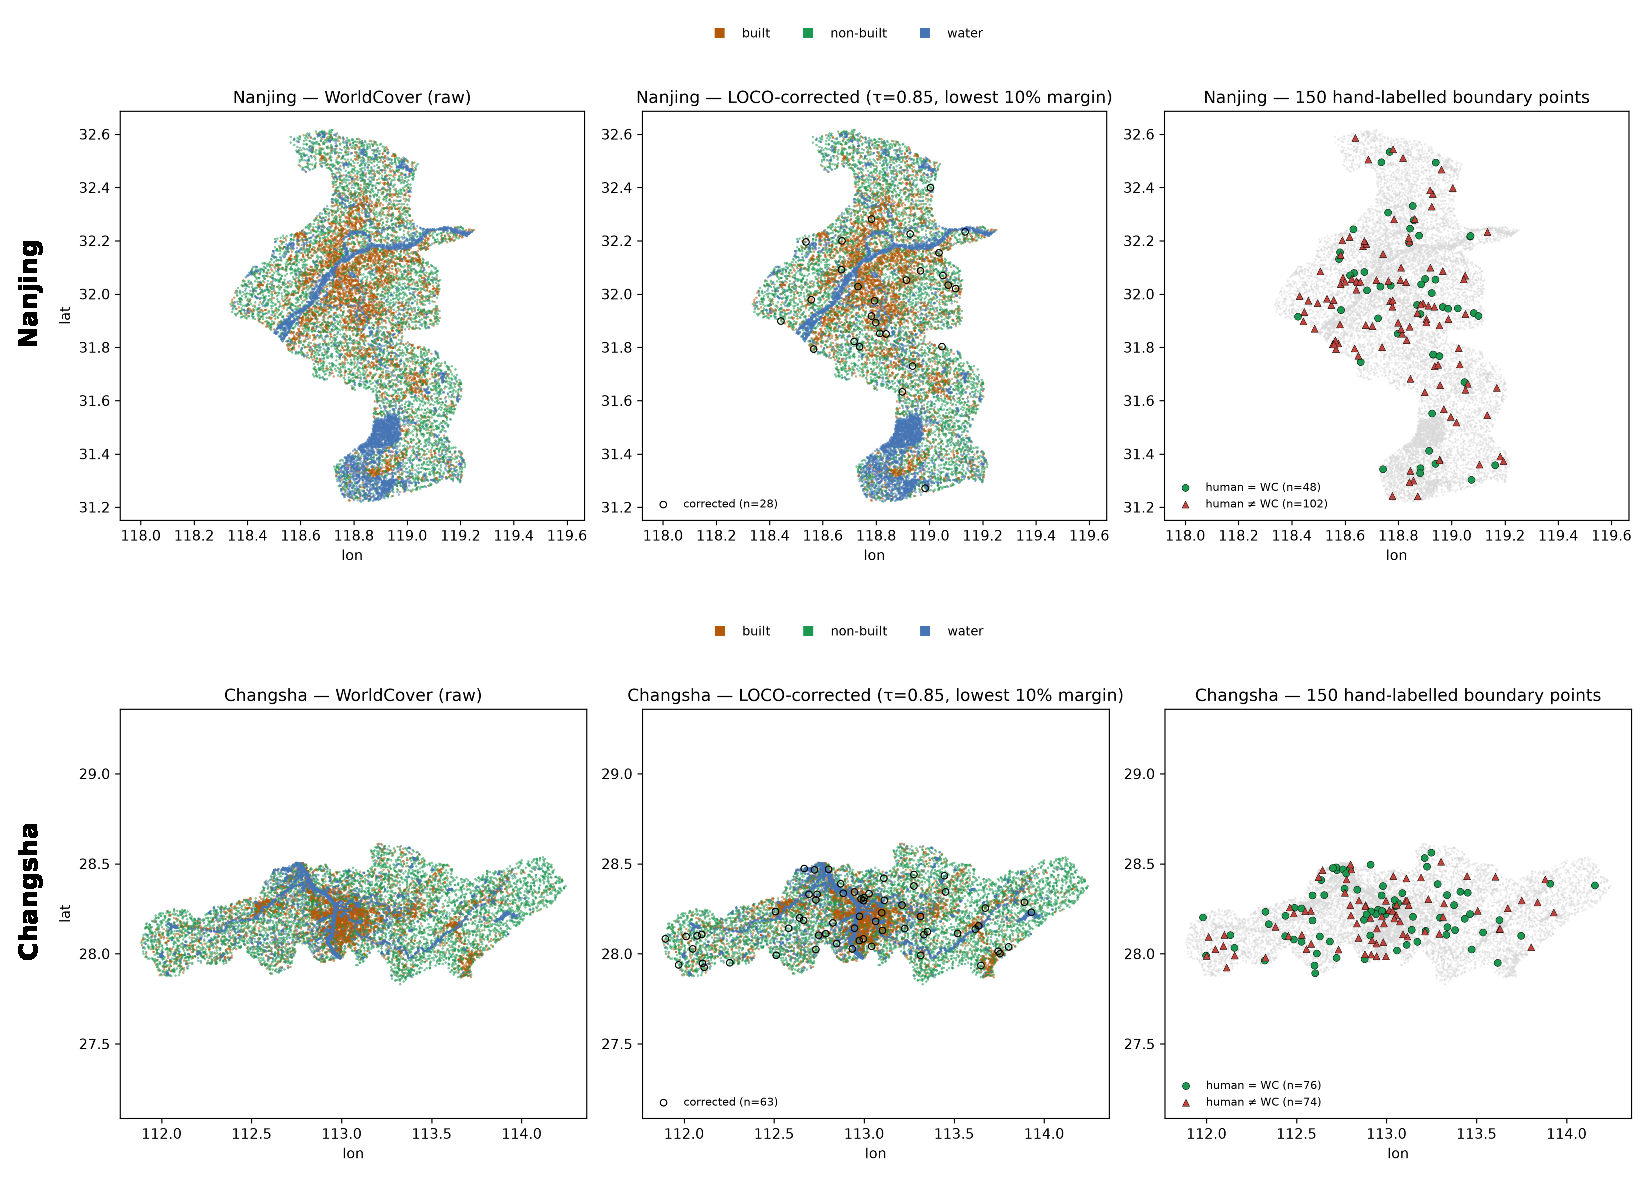
\includegraphics[width=\linewidth]{figures/Figure4_maps_maintext.pdf}
\end{adjustwidth}
\caption{Before/after correction maps for Nanjing (top) and Changsha (bottom),
over the 15,000 stratified city points. (\textbf{A})~raw WorldCover class map;
(\textbf{B})~LOCO-corrected map ($\tau = 0.85$, lowest-decile within-city
margin), the operator's changed points circled (Nanjing 28, Changsha 63);
(\textbf{C})~the 150 expert boundary points, expert\,$=$\,WC (green) vs
expert\,$\neq$\,WC (red; Nanjing 102, Changsha 74), over a faded backdrop.
Nanjing and Changsha are shown because they bracket the operator's
performance range (Section~\ref{sec:results-loco}); the other four cities are
in the Supplementary Material (Figures~S1--S4).
\label{fig:map_maintext}}
\end{figure}

In every city the operator's changes and the expert $\neq$ WC points cluster
along the built-up edge and the river and water margins rather than scattering
across the map. Hangzhou and Nanjing change the fewest points (30 and 28),
consistent with their sparse Phase~3 corrections. This spatial concentration is
qualitative evidence that BAMS
sampling placed the labelling budget on genuine boundary zones
(Section~\ref{sec:disc-scope}); it does not by itself establish that the
disagreement rate there exceeds what random sampling would give.

%% ===================== 5  DISCUSSION ============================
%% =====================================================================
%%  body/discussion.tex  --  Section 5 (Discussion)
%%  Drop-in fragment; compiles only inside the MDPI Remote Sensing template.
%%
%%  Rewritten 3-subsection version: Results re-narration removed; 5.3 (edge)
%%  and 5.4 (LOCO) folded into 5.1; 5.5 limitations kept. The "four
%%  considerations" list now lives here (5.3), moved out of Methods 3.1.
%%  ~1420 w -> ~925 w. No number changed.
%%
%%  2026-09-10 — readability pass (sentence-level only). Split long
%%  subject-verb-separated sentences (esp. 5.1 "Using cross-product
%%  agreement as ... selects a subset"); no claim, number, statistic,
%%  citation or cross-reference changed; every edit information-equivalent.
%%
%%  Cite keys: tuanmu2014 zhangroy2017 wang2024a venter2022 yuan2026 xu2024
%%             zanaga2022 brown2022 karra2021
%%  Labels defined: sec:discussion sec:disc-arbitrate sec:disc-edge
%%                  sec:disc-loco sec:disc-mechanism sec:disc-scope
%%  Labels expected: sec:results sec:sampling sec:results-independence
%%                   app:recheck
%% =====================================================================

\section{Discussion}\label{sec:discussion}

\subsection{Interpretation}\label{sec:disc-arbitrate}

At land-cover class boundaries, in these six cities, agreement among
global products is not evidence of correctness. Each product reproduces the
expert label on fewer than half the candidates, and where Dynamic World and
Esri agree with each other (0.87 of points) that agreement is correlated error,
not corroboration: their error indicators move almost in lockstep (Yule's
$Q = 0.97$, against $\approx 0.08$--$0.14$ for either WorldCover pair), and their consensus
predicts the expert label no better than a single product (0.43 against a 0.45
base rate). The practical consequence is narrow but concrete. Cross-product
agreement is the standard convenience where field data are scarce, used both to
merge consensus products \citep{tuanmu2014} and to harvest training samples
from the pixels where maps agree \citep{zhangroy2017,wang2024a}. Used at this
boundary as a high-confidence signal---the C4 practice this paper set out to
test---it selects a subset no closer to expert judgement than any single
product, and discards disagreement that is itself informative. The spectral-
and temporal-consistency safeguards in these pipelines are not designed to
catch error that is correlated across the products being combined.

That discarded disagreement is directional, not noise\label{sec:disc-edge}.
Once WorldCover assigns ``built-up'' the expert reads non-built about seven
times in ten (0.60--0.79 in every city), and the disagreement concentrates
where built-up meets vegetation---intra-urban green space (71.2\%) is the
single highest group, ahead of road/road edge (64.1\%) and the built-up edge
itself (62.6\%). This echoes the documented
tendency of global products to absorb parks, street trees and residential
greenery into the built class \citep{yuan2026,xu2024}. It is not merely a
schema artefact: Dynamic World's built-area predictions can incorporate urban
vegetation in practice, whereas WorldCover's nominal Built-up class
excludes it \citep{venter2022}, yet
WorldCover still misses it at this rate. This directional error has a specific
consequence for the C4 harvesting practice examined here, reported in
Section~\ref{sec:results-errordir}: a DW\,$=$\,Esri filter retains a sample
whose own class composition changes little, but the agreed label itself, used
as a pseudo-label, severely under-counts non-built cover among those same
points. The bias is mainly
in the mislabelling of the retained points, not in a large shift in which
points agreement happens to retain.

The disagreement is nonetheless structured enough to carry a transferable
signal\label{sec:disc-loco}, evaluated three ways. As an operator-transfer
prediction (Phase 1), a leave-one-city-out operator trained on five
cities predicts the sixth city's expert labels at 0.67--0.75, above both a
do-nothing baseline of 0.32--0.59 and a majority-class baseline of 0.53--0.65
(narrowest margin roughly 0.04--0.05, in Hefei). As a corrected label map
scored directly against the 150 expert points, with no downstream classifier
(Phase 3), it moves 83\% of the points it changes toward the expert (six-city
mean; roughly 17 points per city), against 33\% for the same number of random
flips, and recovers about one-fifth of the OA gain a within-city oracle
achieves on the same evaluation. As training labels for a downstream
classifier (Phase 2), the paired same-city-same-seed gain ($+$0.015 on
average) is swamped by the $\approx$ 10,000 unchanged training points at the
gated thresholds used here---plausibly real (Section~\ref{sec:results-loco}),
but small next to the bulk of the training set. A few dozen boundary
corrections are the right scale for auditing a label map, not for
retraining one.

\subsection{Why Dynamic World and Esri Err Together}\label{sec:disc-mechanism}

The coupling is strong and systematic, and choosing among its possible causes
needs product-internal information that is not published; this paper does not
identify which cause dominates. Three candidates are consistent with what is
public. A shared model family: Dynamic World and Esri are both deep
semantic-segmentation models on Sentinel-2 \citep{brown2022,karra2021}, whereas
WorldCover---a gradient-boosted-tree classifier with a rule-based post-process
\citep{zanaga2022}---is the architectural odd-one-out, whose errors are at most
weakly coupled to either ($Q \approx 0.08$--$0.14$); but WorldCover also differs from the
other two in exact input processing, not architecture alone, so this
comparison does not isolate architecture from shared input. A shared
training-label lineage would produce the same pattern but cannot be
documented from the public record. And shared Sentinel-2 input on its own
does not obviously predict the observed asymmetry, since WorldCover uses the
same imagery without joining the coupling---though, again, WorldCover differs
from Dynamic World and Esri on more than input alone. Which of these
dominates, or whether they combine, is left to future work with access to the
training data and model internals; the statistical fact does not depend on
the answer---the two deep-segmentation products are not two independent
opinions.

\subsection{Scope and Limitations}\label{sec:disc-scope}

\emph{Shared Sentinel-2 basis.} Selection and reference draw on a common
Sentinel-2 information base, so one may question whether Section~\ref{sec:results}
measures product error or Sentinel-2 legibility. Four considerations bound
this: the interpreter integrates spatial configuration, texture, context and a
false-colour infrared view rather than acting as a per-pixel spectral
classifier; three independent interpreters converge on the same labels
(Fleiss' $\kappa = 0.89$); the disagreement concentrates in high-confidence,
interpretable cases; and the sharpest
result---$Q \approx 0.97$ for DW/Esri against $\approx 0.08$--$0.14$ for the WorldCover
pairs (Section~\ref{sec:results-independence})---is a large, asymmetric
differential between product pairs rather than a shift shared uniformly
across all three; we do not have a reference-noise model precise enough to
rule out an expert-dependent contribution to that asymmetry on this basis
alone. An independent blind re-classification of 30 high-confidence
expert $\neq$ WorldCover points reproduced the expert label on 29 and the
WorldCover label on none (Appendix~\ref{app:recheck}), which bears on that
possibility directly.

\emph{Single-annotator reference.} Results that score predictions directly
against the expert label---the confidence stratification, the error-direction
analysis, the arbitration PPV (S2c)---are capped by its reliability most
directly. The excess-agreement and error-dependence checks (S2a, S2b;
Section~\ref{sec:results-independence}) condition on, or define errors
relative to, the expert label rather than scoring a prediction against it
directly; we do not have a reference-noise model precise enough to rank how
tightly each check depends on that reliability, so all three remain
statements about dependence relative to the current expert reference, not an
unconditional one.

\emph{Confidence-stratum bias.} The rise in the expert $\neq$ WorldCover rate
on high-confidence labels (0.53 to 0.67) carries a known upward bias---an
annotator may reserve ``high'' when a product error is obvious. Disagreement
remains high among labels marked as high confidence. Confidence selection may
contribute to this pattern; the blind re-check provides additional evidence
of product error. We do not have a labelling-error model precise
enough to independently bound how large a confidence artefact alone could
produce, so the Nanchang (42/42) and Wuhan (0.88) magnitudes are consistent
with a real effect but not proof of one on this basis alone---the blind
re-classification above (29/30 holding the expert label) is the direct check
on this subset.

\emph{Scene grouping.} The physical-scene rates are a localisation aid, not a
formal stratified sample; the notes are free-text, mapped post hoc to a common
code table, so contrasts are drawn only in the pooled set.

\emph{Geographic and sensor scope.} Six middle- and lower-Yangtze cities, one
climate, one shared Sentinel-2 basis: a bounded existence result, not a prevalence estimate, and in one of
the harder land-cover settings rather than an easy one. Two features travel
beyond the specific numbers. First, per-city expert $=$ WorldCover agreement
ranges from 0.32 to 0.59, yet the direction of the effect is identical in all
six, so it is not a single-city artefact. Second, Dynamic World and Esri are
each trained once and applied globally, so the same coupling could recur
wherever they are used together elsewhere; the strength found here (0.87, $Q
= 0.97$) will not carry over unchanged, and Section~\ref{sec:disc-mechanism}
does not identify which candidate mechanism is responsible. That deployment
fact, not a claim that the mechanism itself transfers, is why replicating the
boundary-aware sampling and the four-way diagnostic in
other climates and urban morphologies is the natural next step.

%% ===================== 6  CONCLUSIONS ===========================
%% =====================================================================
%%  body/conclusions.tex  --  Section 6 (Conclusions)
%%  Drop-in fragment; compiles only inside the MDPI Remote Sensing template.
%%
%%  Rewritten: 3 paragraphs -> 2; the middle number-replay paragraph removed.
%%  ~350 w -> ~180 w. No number changed.
%%
%%  2026-09-10 — readability pass (sentence-level only). Reordered the
%%  opening sentence so "tested whether ..." is not split by the setting
%%  clause; split the ~70-word lockstep sentence and one ";" chain. No
%%  claim, number or citation changed; every edit information-equivalent.
%%
%%  Cite keys: none
%%  Labels defined: sec:conclusions
%% =====================================================================

\section{Conclusions}\label{sec:conclusions}

We tested whether agreement among global 10~m land-cover products arbitrates
the reference label, at land-cover class boundaries and on 900
expert-interpreted points across six middle- and lower-Yangtze cities. It does not. Each of
ESA WorldCover, Dynamic World and Esri Land Cover matches the expert on fewer
than half the boundary candidates. The only agreement that is high across all
six cities---Dynamic World with Esri, 0.87---is correlated error rather than
independent corroboration: the two products' errors move almost in lockstep
(Yule's $Q \approx 0.97$) while WorldCover's errors are at most weakly coupled
to either ($Q \approx 0.08$--$0.14$), and the Dynamic World--Esri consensus does not clearly exceed a
single product's base rate (0.43 against 0.45). The WorldCover error is
directional---once it calls ``built-up'' the expert reads non-built about
seven times in ten. Separately, an agreement-filtered (Dynamic World--Esri)
label set at the boundary also under-represents non-built cover, in the same
direction in every city.

This shows the behaviour exists in six cities sharing one
Sentinel-2 basis, not how
often it occurs elsewhere. The specific coupling
strengths need not carry over, and this paper does not identify which
mechanism drives the coupling (Section~\ref{sec:disc-mechanism}). The practical implication is
narrow: at these boundaries, cross-product agreement should not be used on its own
as a pseudo-reference, a high-confidence training label, or a quality filter,
because the spectral and temporal safeguards in current weak-supervision
pipelines are not built to catch error correlated across the products being
combined. Replicating the boundary-aware sampling and the multi-reference
diagnostic in other climates and urban morphologies is the natural next step.

%% ===================== BACK MATTER =============================
%% MDPI order. Initials (X.X.) and the data/funding specifics are %TODO --
%% they depend on the final author list and repository DOI.

\authorcontributions{Conceptualization, \needsedit{X.X.}; methodology, \needsedit{X.X.};
software, \needsedit{X.X.} and \needsedit{Y.Y.}; formal analysis, \needsedit{X.X.};
investigation, \needsedit{Z.Z.}; validation, \needsedit{W.W.};
writing---original draft preparation, \needsedit{X.X.}; writing---review and editing, \needsedit{W.W.}
All authors have read and agreed to the published version of the manuscript.}
%TODO replace initials with real author names (CRediT). Placeholder mapping:
% X.X. = lead/corresponding author (conceptualization, methodology, software
%        design, formal analysis, original draft); Y.Y. = code implementation
%        (software, hands-on scripting); Z.Z. = data collection/annotation
%        (investigation); W.W. = review role (validation, writing---review
%        and editing).

\funding{\needsedit{This research received no external funding.}} %TODO confirm, or replace
% with ``This research was funded by NAME OF FUNDER grant number XXX''.

\institutionalreview{Not applicable.}

\informedconsent{Not applicable.}

\dataavailability{The three global land-cover products are publicly available
through Google Earth Engine: ESA WorldCover 2021 v200
(\href{https://developers.google.com/earth-engine/datasets/catalog/ESA_WorldCover_v200}{\path{ESA/WorldCover/v200}}), Dynamic World
(\href{https://developers.google.com/earth-engine/datasets/catalog/GOOGLE_DYNAMICWORLD_V1}{\path{GOOGLE/DYNAMICWORLD/V1}}), and Esri/Impact Observatory 10~m Land Cover
(\href{https://gee-community-catalog.org/projects/S2TSLULC/}{\path{projects/sat-io/open-datasets/landcover/ESRI_Global-LULC_10m_TS}}).
The Sentinel-2 Level-2A surface-reflectance archive
(\href{https://developers.google.com/earth-engine/datasets/catalog/COPERNICUS_S2_SR_HARMONIZED}{\path{COPERNICUS/S2_SR_HARMONIZED}}) is likewise public. The 900
expert-interpreted boundary points, the boundary-aware sampling code, and the
diagnostic and leave-one-city-out analysis scripts are organised as a single
code-plus-data repository: analysis code in \path{scripts/}; the six
cities' data (original 15{,}000-point pools through the final corrected
labels) in \path{data/cities/}; cross-city reference data (Dynamic
World/Esri second reference, scene grouping) in
\path{data/shared_reference/}; script outputs in
\path{data/analysis_outputs/}; and the inter-annotator blind re-check in
\path{data/interannotator_recheck/}. This repository will be archived at
\needsedit{\url{https://doi.org/XXXX}} upon publication.} %TODO repository DOI once minted (structure above is now fixed; only the DOI itself is a placeholder)

\acknowledgments{During the preparation of this manuscript, the authors used a
large language model (Claude, Anthropic) for LaTeX formatting and
language editing. The authors have reviewed and edited the output and take full
responsibility for the content of this publication.}

\conflictsofinterest{The authors declare no conflicts of interest.}

\appendixtitles{yes}

\appendixstart

\appendix

%% ===================== APPENDIX A ==============================
%% =====================================================================
%%  body/appendix.tex  --  Appendix A (Blind Re-Check of High-Confidence
%%  Disagreements)
%%  Drop-in fragment; compiles only inside the MDPI Remote Sensing template.
%%
%%  The master file issues \appendix once, before \input-ing this file.
%%
%%  2026-09-10 — readability pass (sentence-level only). Split two ";"
%%  chains; moved the second analyst's credentials out of a subject-verb
%%  em-dash aside into a following sentence.
%%  2026-09-10 (2) — "293 candidates" -> "281 under the final labelling (293
%%  when the check was run)"; the Hangzhou re-labelling (two-stage rule)
%%  shifted the high-confidence expert!=WC subset. The 30 checked points are
%%  unchanged and all remain high-confidence expert!=WC; the 29/30 result
%%  stands.
%%
%%  Cite keys: none
%%  Labels defined: app:recheck
%%  Labels expected: sec:results-confidence sec:sampling sec:results-errordir
%% =====================================================================

\section{Blind Re-Check of High-Confidence Disagreements}\label{app:recheck}

\paragraph{Purpose.} To check whether the high-confidence expert $\neq$
WorldCover disagreements of Section~\ref{sec:results-confidence} could be an
artefact of the original single annotator, rather than WorldCover error. This
is separate from, and additional to, the 120-point three-colleague reliability
exercise of Section~\ref{sec:sampling}.

\paragraph{Point selection.} From the multi-reference table, points with a
high-confidence expert label and $\text{expert} \neq \text{WorldCover}$ were
retained. Thirty were then drawn for the check---five per city, in decreasing
BAMS classifier margin ($5 \times 6$ cities). The subset numbers 281 points
under the final reference labelling (293 when the check was run, before the
Hangzhou re-labelling); all 30 checked points remain high-confidence
expert $\neq$ WorldCover points.

\paragraph{Protocol.} A second analyst re-classified all 30 points into
\{built-up, non-built, water\} from sub-metre Google satellite imagery together
with the 2021 Sentinel-2 composite. This analyst had remote-sensing land-cover
interpretation experience and had not taken part in the original reference
labelling. The stepper script was modified to hide the \texttt{expert} and
\texttt{wc} fields, so the analyst was blind to both the original expert label
and the WorldCover label. The returned classes were cross-tabulated against the
original expert label afterwards.

\paragraph{Result.} The second analyst's blind classification matched the
original expert label on \textbf{29 of the 30 points} and the WorldCover label
on \textbf{none}. The single unresolved point (Changsha, \texttt{Original\_ID}
10031; expert $=$ non-built, WorldCover $=$ water) is an edge/mixed pixel the
analyst could not assign a confident class to from the available imagery. Of
the 30 points, 20 are cases where the expert reads non-built (WorldCover called
19 of them built-up and one water), 6 where the expert reads water (WorldCover
called five non-built and one built-up), and 4 where the expert reads built-up
(WorldCover called all four non-built)---the same directional pattern as the
pooled WorldCover $\to$ expert confusion matrix of
Section~\ref{sec:results-errordir}.

\paragraph{What it does and does not establish.} It removes the same-analyst
circularity in attributing the high-confidence disagreements to WorldCover. It
is not a fully independent measurement: the original labelling protocol already
consulted the same Google high-resolution basemap as ancillary context, so the
second analyst is an independent \emph{judgement} sharing the same imagery
sources. Fully cross-independent annotation at scale is the separate
reliability exercise reported in Section~\ref{sec:sampling}.

%% ===================== APPENDIX B ==============================
%% =====================================================================
%%  Supplementary Material, folded into the single-file submission per
%%  user instruction (2026-09-11): do not maintain a separate
%%  manuscript_supplementary.tex file. Content ported from
%%  docs/manuscript_supplementary.md (S1-S6); keep both in sync when
%%  numbers change (see submission/README.md).
%%
%%  Cite keys: none
%%  Labels defined: app:supp tab:S1 tab:S3 tab:S4 tab:S5 tab:S6
%%    fig:map_s1 fig:map_s2 fig:map_s3 fig:map_s4 fig:S5chips
%%  Labels expected (referenced from main text as plain "Table~SN" /
%%    "Figure~SN" text, not \ref, so no cross-file breakage if renumbered):
%%    sec:results-loco sec:results-independence
%%
%%  2026-09-12 -- format check: MDPI's \appendix does NOT auto-number
%%  tables/figures as "S1, S2, ..."; left alone, Table/Figure counters
%%  here would render as plain continuations of the main-text numbering
%%  (e.g. "Table 7"), which would not match the ~10 hardcoded "Table SN" /
%%  "Figure SN" mentions in the main text and in this section's own
%%  headings. Added a local \thetable/\thefigure rename + counter reset
%%  right after \section{Supplementary Material} so the auto-numbering
%%  actually prints "Table S1".."S6" / "Figure S1".."S5", matching every
%%  existing reference. Scope is local to this section (Appendix A above
%%  has no tables/figures, so it is unaffected either way).
%% =====================================================================

\section{Supplementary Material}\label{app:supp}

\renewcommand{\thetable}{S\arabic{table}}
\renewcommand{\thefigure}{S\arabic{figure}}
\setcounter{table}{0}
\setcounter{figure}{0}

Unless noted otherwise, every ``Source:'' below is relative to
\path{docs/results_snapshot/}, the frozen snapshot backing every number in
this paper. Table~\ref{tab:S5} is the one exception, drawn from the live
pipeline output in \path{data/analysis_outputs/} instead, because it reports
a majority-class baseline column added after the snapshot was taken.

\subsection{LOCO Operator: Gate-Sensitivity Sweep (Phase 2b)}\label{app:supp-s1}

Referenced from Section~\ref{sec:results-loco}. The proposed downstream
correction (transferred operator, boundary- and confidence-gated) moves the
six-city mean overall accuracy against the 150 expert points from 0.375 to
only 0.389, inside the pooled city-and-seed standard deviation (0.07;
Section~\ref{sec:results-loco} decomposes it: the seed-only component is an
order of magnitude smaller). Table~\ref{tab:S1}
varies the confidence threshold $\tau$ and the within-city margin quantile $q$
that gates which candidates are eligible for correction, and reports the
six-city mean downstream overall accuracy against the expert labels
(Human-OA) and against WorldCover (WC-OA), together with the mean number of
labels rewritten within the $\approx$10,000-point non-boundary training
subset used to retrain the downstream classifier (Section~\ref{sec:loco},
Phase 2). This is a different, smaller population than the $\approx$15,000-point
full city map that Table~\ref{tab:S6} reports changes against
(Table~\ref{tab:S5} is scored on the 150 expert points per city, not the full
map): the margin quantile $q$ here is taken over the training subset's own margins,
not the full city's, so the two point counts are not directly comparable even
at matching $\tau$ and $q$.

\begin{table}[H]
\caption{Gate sensitivity, six-city mean. Source:
\protect\path{loco_correction_operator/phase2b_sweep_summary.csv}.\label{tab:S1}}
\begin{adjustwidth}{-\extralength}{0cm}
\centering
\small
\begin{tabularx}{\fulllength}{CCCCC}
\toprule
\boldmath$\tau$ & \boldmath$q$ & \textbf{Points changed (of the $\approx$10,000-pt training subset)}
& \textbf{Human-OA} & \textbf{WC-OA}\\
\midrule
baseline & --- & 0   & 0.375 & 0.929\\
0.90 & 0.05 & 1   & 0.375 & 0.929\\
0.90 & 0.10 & 5   & 0.379 & 0.929\\
0.90 & 0.20 & 8   & 0.382 & 0.929\\
0.85 & 0.05 & 9   & 0.379 & 0.929\\
0.85 & 0.10 & 23  & \textbf{0.389} & 0.929\\
0.85 & 0.20 & 41  & 0.405 & 0.928\\
0.80 & 0.10 & 60  & 0.408 & 0.928\\
0.80 & 0.20 & 112 & 0.449 & 0.925\\
0.70 & 0.10 & 186 & 0.454 & 0.923\\
0.70 & 0.20 & 345 & 0.516 & 0.913\\
\bottomrule
\end{tabularx}
\end{adjustwidth}
\end{table}

Reaching $+$14 points of downstream Human-OA (0.375 $\to$ $\approx$0.516)
requires loosening to $\tau = 0.70$, $q = 0.20$ and rewriting $\approx$345 of
the $\approx$10,000-point training subset, at a drop of $\approx$1.5 points in
agreement with raw WorldCover (WC-OA; 0.929 $\to$ 0.913)---a shift away from
WC, not necessarily an accuracy cost.
At the gated thresholds used in the main text ($\tau \ge 0.85$, chosen for
high firing precision rather than a guarantee of calibrated reliability), the
downstream improvement is small, with gains in five of the six cities. A few
dozen boundary-label corrections do not move a random forest trained on
$\approx$10,000 points by much; this is why the label-map referee
(Section~\ref{sec:results-loco}, Phase~3) evaluates the corrected map
directly rather than through a retrained classifier.

\subsection{LOCO Operator: Reduced Feature Subset (\texttt{transfer15})}\label{app:supp-s2}

Referenced from Section~\ref{sec:results-loco}. The main-text operator uses a
27-feature vector (nine point-level spectral features plus their nine
$3\times3$ neighbourhood means and nine $3\times3$ neighbourhood standard
deviations). The \texttt{transfer15} variant drops the six raw reflectance
bands and their neighbourhood means---which carry cross-city radiometric
offsets---keeping the three spectral indices and all nine neighbourhood
standard-deviation terms. \texttt{transfer15} is slightly worse than the full
27-feature operator in every city (operator-vs-expert agreement lower by
roughly 0.02--0.05), so the raw reflectance bands remain useful for the
transfer despite the radiometric offsets. The main text reports only the
27-feature operator. Source:
\path{loco_correction_operator/phase1_corrector_transfer.csv}
(\texttt{feature\_set} column: \texttt{all27} vs \texttt{transfer15}).

%% Skip table number 2: "Table S2" (product error-dependence) was promoted
%% into the main text (Table~\ref{tab:S2}, Section~\ref{sec:results-independence})
%% and is cited there under its own main-sequence number, not as "S2". The
%% next table here is still cited throughout as "Table S3" (e.g. line
%% ~1297), so the counter must jump 1 -> 3 to keep that numbering correct.
\addtocounter{table}{1}

\subsection{Independence Diagnostic: Confound-Check Tables}\label{app:supp-s3}

Referenced from Section~\ref{sec:results-independence}. The main text states
the conclusions; the full tables are below. The negative-control comparison
(WorldCover shares the Sentinel-2 input with Dynamic World and Esri but not
the deep-segmentation model family, and its excess agreement is about half
that of DW $=$ Esri with error $Q \approx 0.08$--$0.14$) uses quantities already
tabulated in main text Table~\ref{tab:S2} and is not repeated here.

\paragraph{Ontology.} Table~\ref{tab:S3} gives DW $=$ Esri agreement and the
DW $=$ Esri $-$ Human $=$ DW gap under three class schemes, six-city pool
($n = 900$; water points dropped for the third scheme, $n = 623$).

\begin{table}[H]
\caption{Collapsing the class ontology leaves DW $=$ Esri at 0.87--0.92 and
the gap at 0.34--0.48: the coupling is not an artefact of the three-class
remap. The built-vs-non-built row (previously mislabelled ``built vs
vegetation''---the non-built class also contains bare land and other
non-vegetated cover, Section~\ref{sec:products}) drops a point if any source
calls it water. Source:
\protect\path{independence_diagnostic/S3a_ontology_confound.csv}.\label{tab:S3}}
\begin{adjustwidth}{-\extralength}{0cm}
\centering
\small
\begin{tabularx}{\fulllength}{L{2}M{0.75}M{0.75}M{0.75}M{0.75}}
\toprule
\textbf{Scheme} & \textbf{DW $=$ Esri} & \textbf{Human $=$ DW}
& \textbf{Human $=$ Esri} & \textbf{Gap}\\
\midrule
Three-class (built / non-built / water) & 0.874 & 0.446 & 0.422 & 0.429\\
Two-class (built vs rest) & 0.908 & 0.568 & 0.538 & 0.340\\
Built vs non-built (water points dropped) & 0.917 & 0.440 & 0.417 & 0.477\\
\bottomrule
\end{tabularx}
\end{adjustwidth}
\end{table}

\paragraph{Acquisition date, by scene type.} Table~\ref{tab:S4} resolves DW
$=$ Esri agreement by physical scene group, pooled over the 891 boundary
points with a resolvable scene note, groups with $n \ge 15$.

\begin{table}[H]
\caption{The DW $=$ Esri rate stays in 0.83--0.98 across every scene group and
is \emph{highest} in the hardest transition zones (urban green space 0.98,
mixed / complex 0.96) rather than concentrated in the spectrally stable
classes; the coupling is not confined to one kind of scene, though acquisition
timing itself is not tested directly here. Source:
\protect\path{independence_diagnostic/S3c_coupling_by_scene.csv}.\label{tab:S4}}
\begin{adjustwidth}{-\extralength}{0cm}
\centering
\small
\begin{tabularx}{\fulllength}{L{2}M{0.75}M{0.75}M{0.75}M{0.75}}
\toprule
\textbf{Scene group} & \textbf{\emph{n}} & \textbf{DW $=$ Esri}
& \textbf{Human $=$ DW} & \textbf{Gap}\\
\midrule
Urban green space & 52 & 0.981 & 0.135 & 0.846\\
Mixed / complex & 25 & 0.960 & 0.280 & 0.680\\
Built-up edge / urban fabric & 174 & 0.943 & 0.828 & 0.115\\
Cropland / paddy transition & 16 & 0.938 & 0.125 & 0.812\\
Rural settlement / surfaces & 41 & 0.878 & 0.244 & 0.634\\
Bare land / construction & 88 & 0.852 & 0.205 & 0.648\\
Paddy / cropland / field & 19 & 0.842 & 0.316 & 0.526\\
Vegetation / forest edge & 130 & 0.831 & 0.215 & 0.615\\
Road / road edge & 117 & 0.829 & 0.427 & 0.402\\
Water / water edge & 211 & 0.829 & 0.578 & 0.251\\
\bottomrule
\end{tabularx}
\end{adjustwidth}
\end{table}

\subsection{LOCO Correction Operator: Per-City Detail}\label{app:supp-s4}

Referenced from Section~\ref{sec:results-loco}. Table~\ref{tab:S5} gives the Phase~1
operator-transfer numbers behind the ``0.67 to 0.75 against a baseline of
0.32 to 0.59'' range quoted in the main text; Table~\ref{tab:S6} gives the
per-city operator-change and expert $\neq$ WC counts behind main text
Figure~\ref{fig:map_maintext} (Nanjing, Changsha) and
Figures~\ref{fig:map_s1}--\ref{fig:map_s4} below (the other four cities).

\begin{table}[H]
\caption{Phase~1 operator transfer, per city. ``WC $\leftrightarrow$ expert''
is the raw do-nothing baseline agreement (150 boundary points per city).
``Majority-class baseline'' always predicts non-built, learned from the other
five cities' human labels (same leak-proof, leave-one-city-out pattern as the
operator itself; contextualises the operator's gain against class imbalance
alone, since non-built is the majority class pooled across cities).
``Operator $\leftrightarrow$ expert'' is the transferred operator's agreement
with the expert label. Confident firings are predictions with
$p_{\max} \ge 0.85$ and predicted class $\neq$ WC; firing precision is the
fraction of those firings that match the expert label. Source:
\protect\path{data/analysis_outputs/loco_correction_operator/phase1_corrector_transfer.csv}
(live pipeline output, not the frozen snapshot; see note above).\label{tab:S5}}
\begin{adjustwidth}{-\extralength}{0cm}
\centering
\small
\begin{tabularx}{\fulllength}{lCCCCC}
\toprule
\textbf{City} & \textbf{WC $\leftrightarrow$ expert}
& \textbf{Majority-class baseline} & \textbf{Operator $\leftrightarrow$ expert}
& \textbf{Confident firings ($\tau=0.85$)} & \textbf{Firing precision vs expert}\\
\midrule
Wuhan    & 0.41 & 0.53 & 0.71 & 18 & 0.78\\
Hefei    & 0.51 & 0.63 & 0.67 & 28 & 0.68\\
Nanchang & 0.46 & 0.65 & 0.73 & 11 & 0.82\\
Nanjing  & 0.32 & 0.55 & 0.74 & 15 & 0.93\\
Changsha & 0.51 & 0.55 & 0.75 & 18 & 0.83\\
Hangzhou & 0.59 & 0.53 & 0.75 & 11 & 0.91\\
\bottomrule
\end{tabularx}
\end{adjustwidth}
\end{table}

\begin{table}[H]
\caption{Per-city operator-change and expert $\neq$ WC counts underlying the
before/after maps (main text Figure~\ref{fig:map_maintext};
Figures~\ref{fig:map_s1}--\ref{fig:map_s4} below). ``Operator changes'' is the
number of the $\approx$15,000 stratified city points the gated operator
($\tau=0.85$, lowest-decile within-city margin) overwrites relative to raw
WorldCover. Source: \protect\path{loco_correction_operator/}.\label{tab:S6}}
\centering
\small
\begin{tabularx}{0.75\fulllength}{lCC}
\toprule
\textbf{City} & \textbf{Operator changes (of $\approx$15,000)}
& \textbf{Expert $\neq$ WC (of 150)}\\
\midrule
Nanjing  & 28 & 102\\
Changsha & 63 & 74\\
Wuhan    & 35 & 88\\
Hefei    & 91 & 74\\
Nanchang & 38 & 81\\
Hangzhou & 30 & 61\\
\bottomrule
\end{tabularx}
\end{table}

\paragraph{Figures~S1--S4: before/after correction maps, remaining four
cities.} Companion to main text Figure~\ref{fig:map_maintext} (Nanjing,
Changsha; Section~\ref{sec:results-loco}). Each figure: (\textbf{A})~raw
WorldCover class map over the $\approx$15,000 stratified city points;
(\textbf{B})~LOCO-corrected map ($\tau=0.85$, lowest-decile within-city
margin), the operator's changed points circled; (\textbf{C})~the 150 expert
boundary points, expert $=$ WC (green) vs expert $\neq$ WC (red), over a
faded backdrop of the full point set.

\begin{figure}[H]
\begin{adjustwidth}{-\extralength}{0cm}
\centering
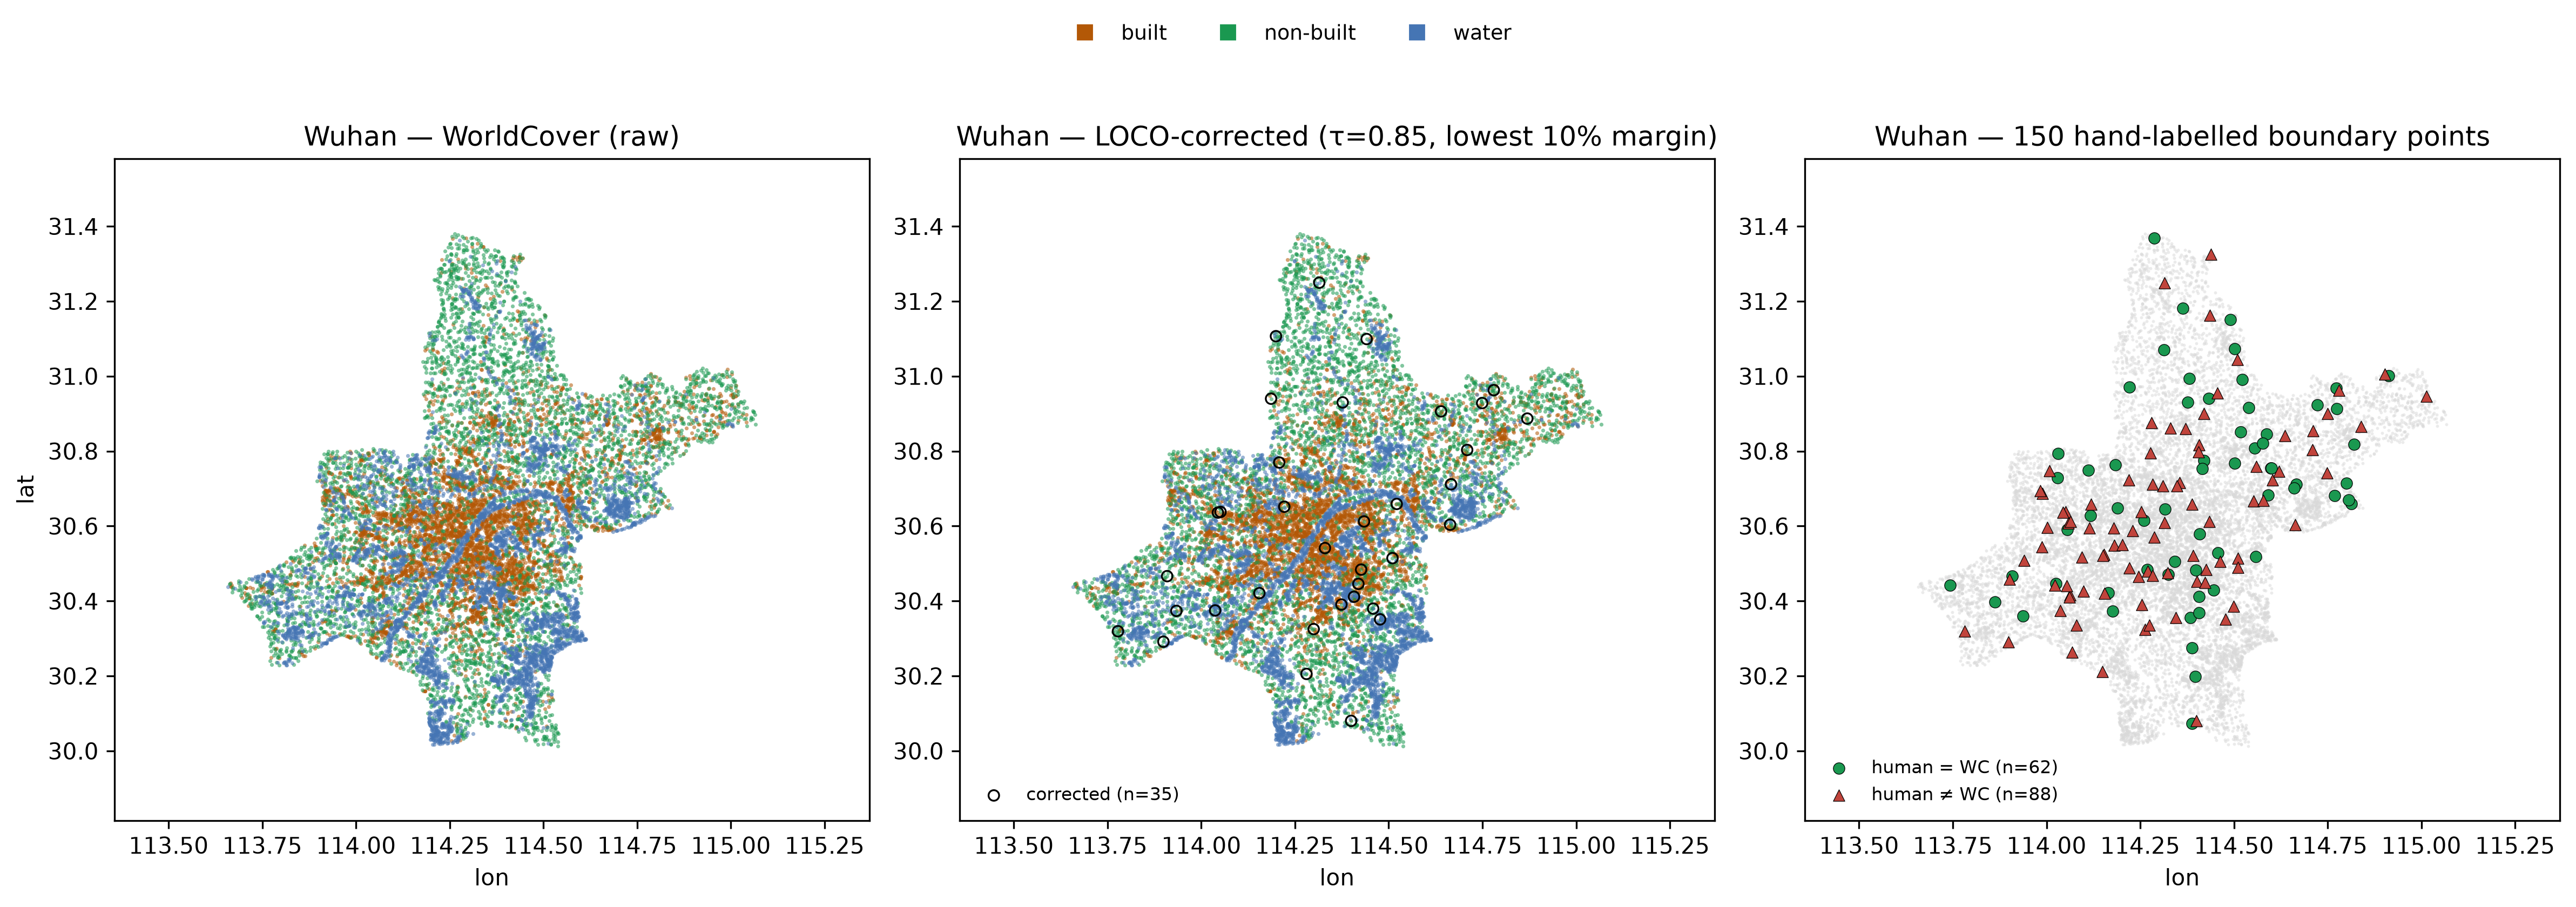
\includegraphics[width=\linewidth]{figures/FigureS1_map_Wuhan.png}
\end{adjustwidth}
\caption{Wuhan before/after correction maps. (\textbf{A})~raw WorldCover;
(\textbf{B})~LOCO-corrected, 35 points changed; (\textbf{C})~150 expert
boundary points, expert $=$ WC (green, $n=62$) vs expert $\neq$ WC
(red, $n=88$).\label{fig:map_s1}}
\end{figure}

\begin{figure}[H]
\begin{adjustwidth}{-\extralength}{0cm}
\centering
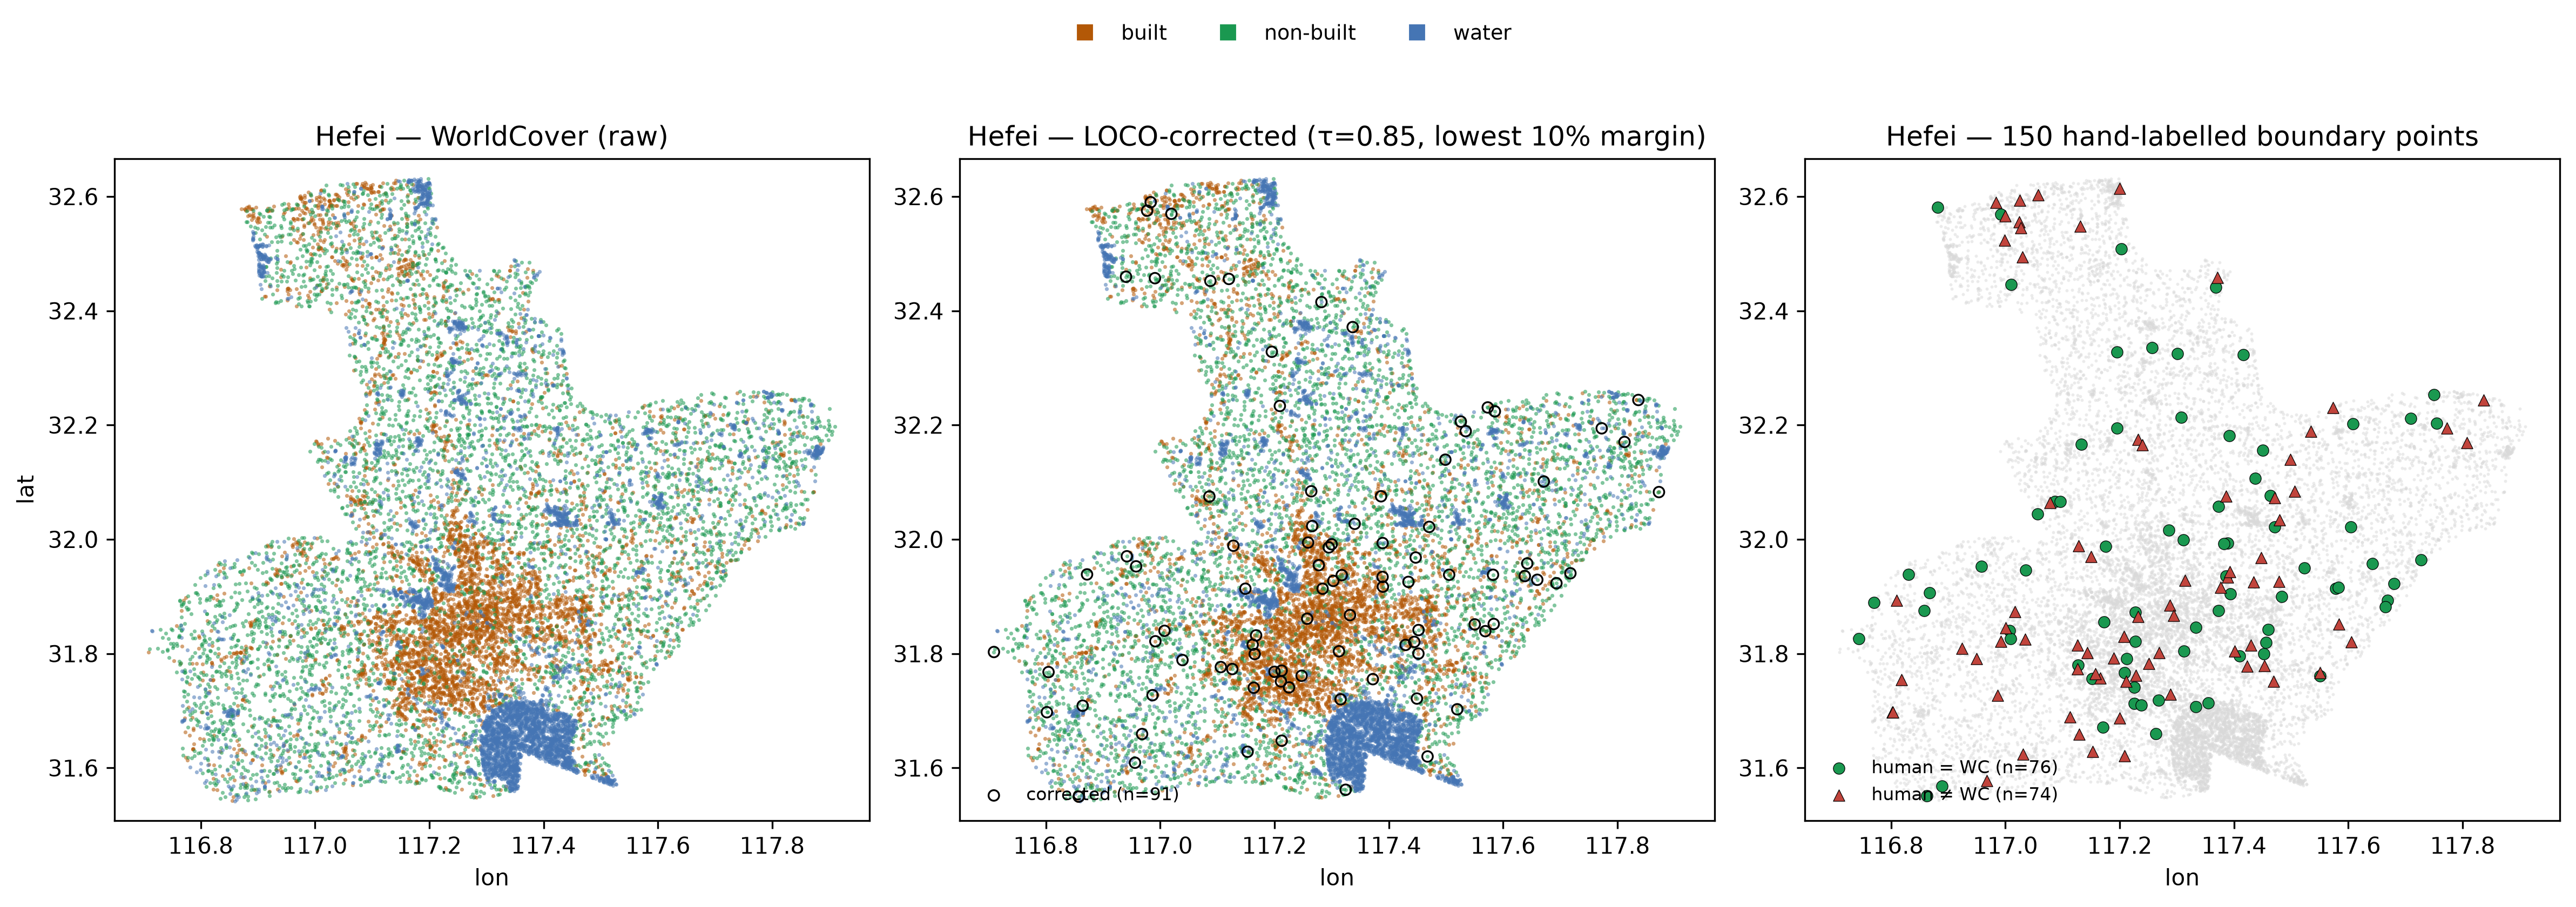
\includegraphics[width=\linewidth]{figures/FigureS2_map_Hefei.png}
\end{adjustwidth}
\caption{Hefei before/after correction maps. (\textbf{A})~raw WorldCover;
(\textbf{B})~LOCO-corrected, 91 points changed; (\textbf{C})~150 expert
boundary points, expert $=$ WC (green, $n=76$) vs expert $\neq$ WC
(red, $n=74$).\label{fig:map_s2}}
\end{figure}

\begin{figure}[H]
\begin{adjustwidth}{-\extralength}{0cm}
\centering
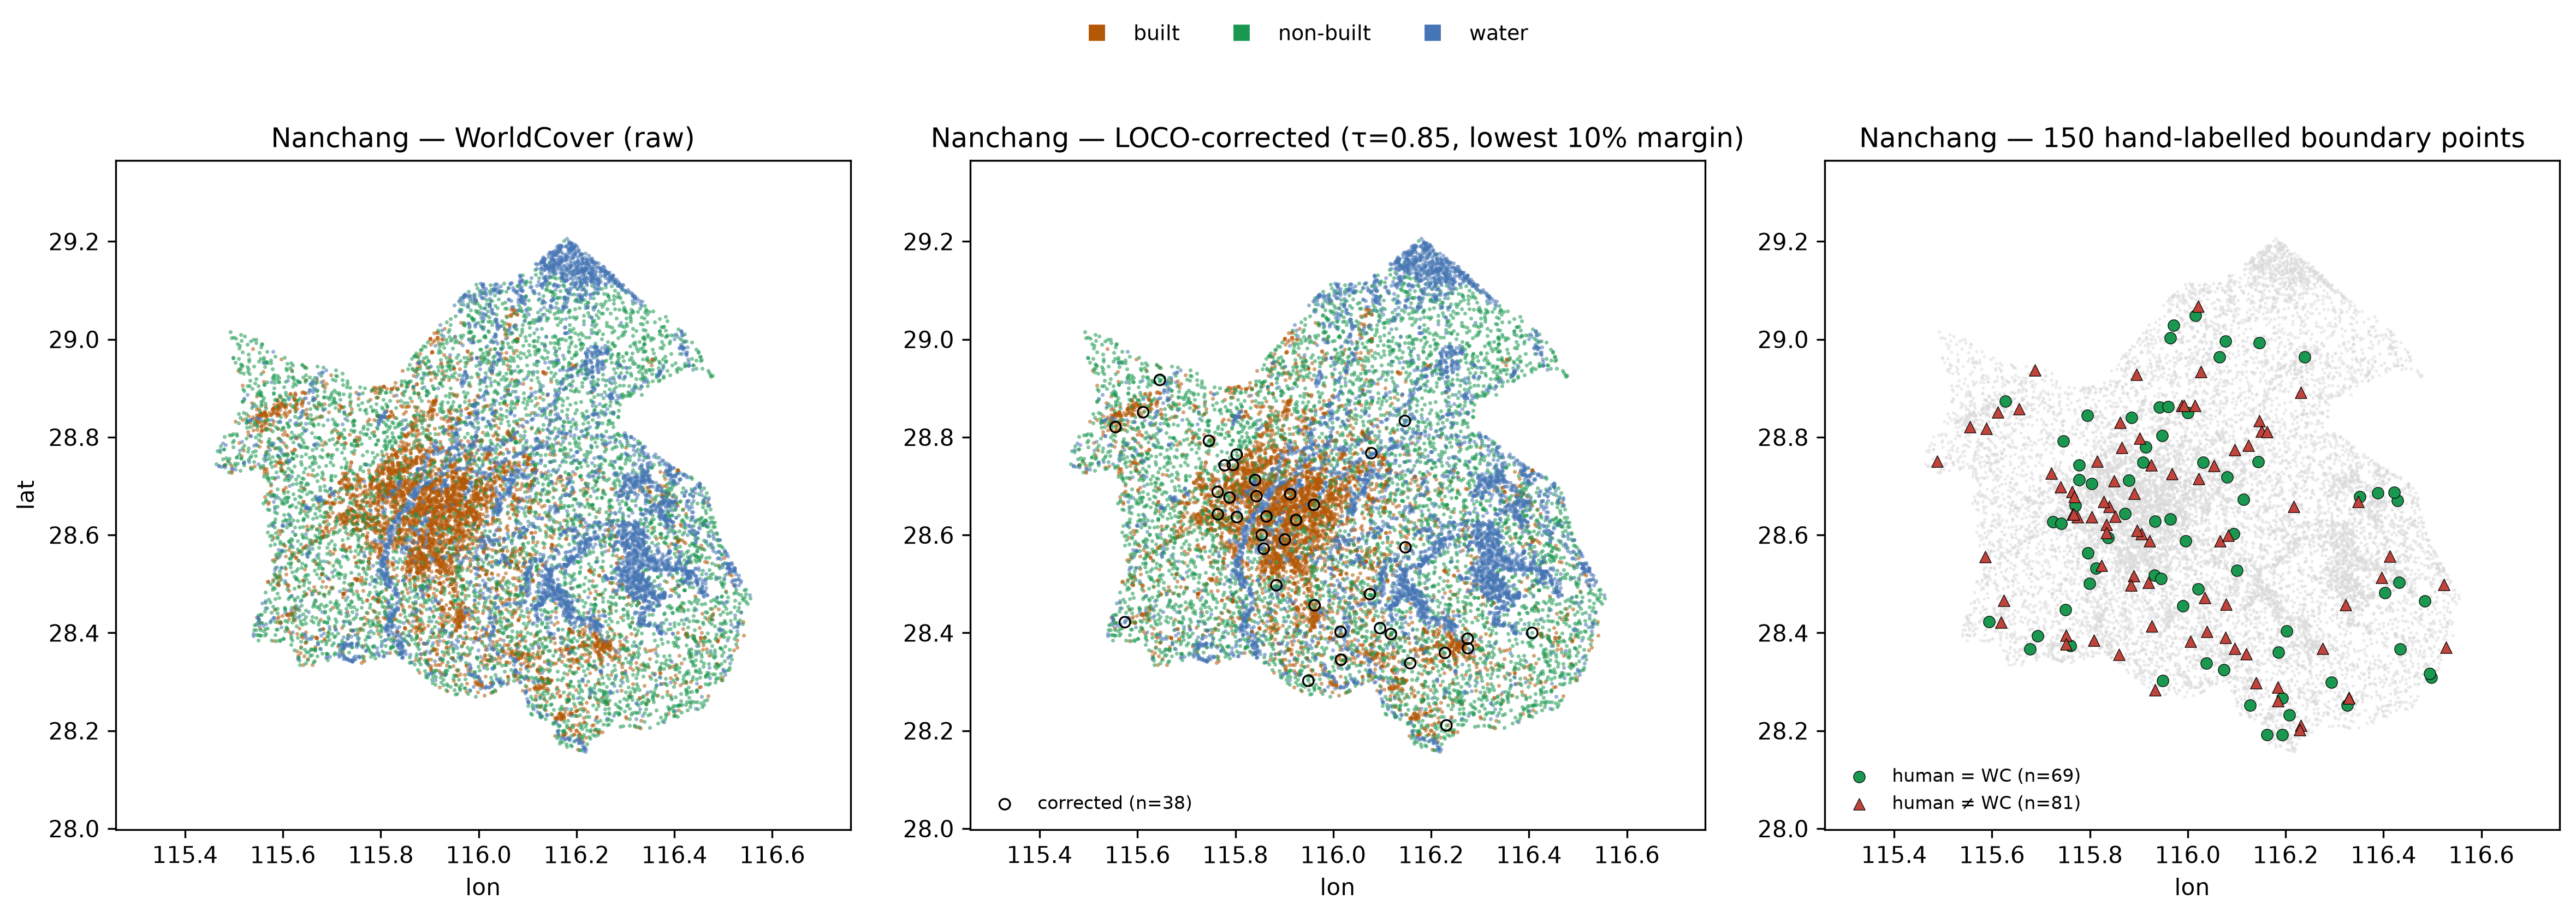
\includegraphics[width=\linewidth]{figures/FigureS3_map_Nanchang.png}
\end{adjustwidth}
\caption{Nanchang before/after correction maps. (\textbf{A})~raw WorldCover;
(\textbf{B})~LOCO-corrected, 38 points changed; (\textbf{C})~150 expert
boundary points, expert $=$ WC (green, $n=69$) vs expert $\neq$ WC
(red, $n=81$).\label{fig:map_s3}}
\end{figure}

\begin{figure}[H]
\begin{adjustwidth}{-\extralength}{0cm}
\centering
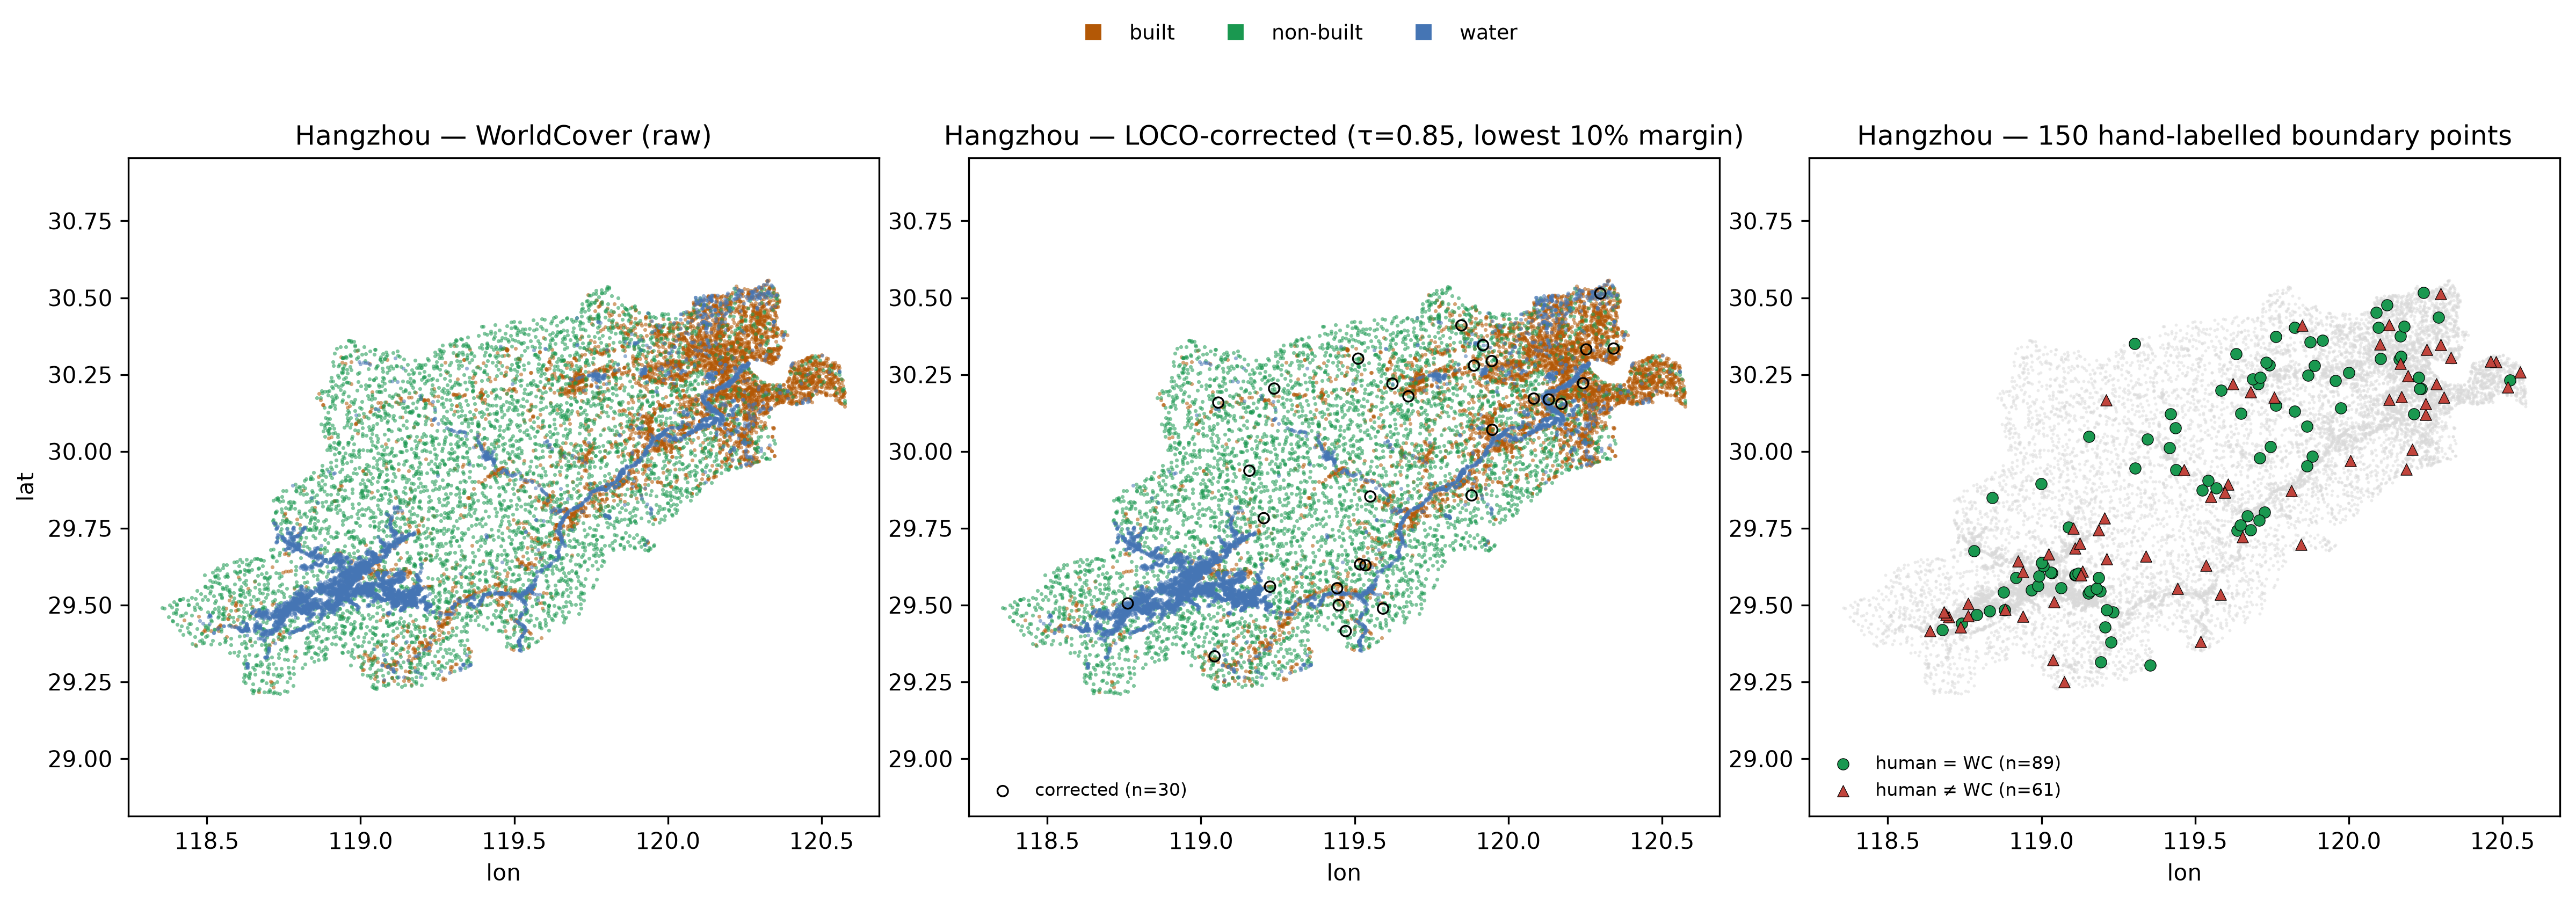
\includegraphics[width=\linewidth]{figures/FigureS4_map_Hangzhou.png}
\end{adjustwidth}
\caption{Hangzhou before/after correction maps. (\textbf{A})~raw WorldCover;
(\textbf{B})~LOCO-corrected, 30 points changed; (\textbf{C})~150 expert
boundary points, expert $=$ WC (green, $n=89$) vs expert $\neq$ WC
(red, $n=61$).\label{fig:map_s4}}
\end{figure}

\subsection{Within-City Label Propagation Leaks (Prototype Expansion)}\label{app:supp-s5}

Referenced from Section~\ref{sec:sampling}. Before adopting the
leave-one-city-out design, we tested within-city propagation of the boundary
labels to their spectral neighbours (our variant of the prototype /
pseudo-label rectification-and-expansion family; ``Prototype Expansion'').

\begin{itemize}
\item \textbf{Leakage diagnostic.} Across five cities and neighbourhood
sizes $K \in \{5, 10, 20, 30\}$, the fraction of expanded points whose
spectral neighbours crossed the evaluation set was $\text{leak\_fraction} =
1.0$ in every configuration: without a spatial partition, every propagated
label draws on a point that is also being scored.
\item \textbf{Leak-proof re-run.} With the train/test split drawn by spatial
block and the evaluation points explicitly removed from the neighbour
search, the procedure produced $n_{\text{expanded}} = 0$---no valid
expansions survive.
\item \textbf{Apparent gain was the classifier swap, not propagation.} In the
non-partitioned runs the ``PE\_Boundary'' scheme reported overall accuracy
0.924 / Boundary Error 227 against 0.914 / 276 for the raw-WC baseline, but
with $n_{\text{expanded}} = 0$ under the leak-proof control that
$\approx +1$ point is attributable to the RF$\to$MLP classifier change and to
treating the 150 hand labels as anchors, not to neighbour propagation.
\end{itemize}

Source: \path{leak_diagnostic/} (\path{leak_diagnostic.csv},
\path{spatial_block_results.csv}, \path{spatial_block_summary.csv}), the
frozen output of a one-off diagnostic run. The generating script lived in an
earlier, non-version-controlled working directory and no longer exists in a
form that can be republished; the CSVs above are preserved as the record of
that check.

\subsection{Illustrative Example Chips: WorldCover Boundary Error (C1/C2)}\label{app:supp-s6}

Referenced from Section~\ref{sec:results-errordir}. Table~\ref{tab:T3}
there establishes the quantitative claim: once WorldCover calls a boundary
point ``built-up'', the expert reads non-built about seven times in ten
($P(\text{expert}=\text{non-built} \mid \text{WC}=\text{built}) = 0.71$).
That number says nothing about what the error looks like on the ground.
Figure~\ref{fig:S5chips} puts real Sentinel-2 imagery behind it---24 boundary
points across the six cities, ranked by a stated margin rule and then
narrowed by a disclosed visual-review pass (below), not picked
freehand---so a reader can see the error, not just read its rate. The
gallery is illustration only; it adds no statistic the main text does not
already report, and no claim in this paper rests on it.

\paragraph{What the three panels show.} Panel \textbf{A}---consensus error
(supports C1 and C2), 12 points, 2 per city---is the figure's core case:
WorldCover, Dynamic World and Esri all call the point built-up, and the
expert reads non-built. This is not a rare corner case: it is the common
outcome in the WC$=$built $\wedge$ expert$=$non-built cell of the reference
table (164 of 197 such points, 83\%). It illustrates C2 directly
(WorldCover's directional error) and C1 by extension, since all three
products land on the same wrong answer at once. Panel \textbf{B}---coupled-pair
error (supports C1), 6 points, 1 per city---isolates the C1 argument on its
own: Dynamic World and Esri, the two products whose errors are most
correlated with each other (Section~\ref{sec:results-independence}), both
call the point built-up and both are wrong; WorldCover---the product least
coupled to the other two---dissents and is correct. Read together, panels A
and B show what ``agreement is not independent corroboration'' means in
practice. In A, three products agree and are still wrong. In B, the two
most-correlated products agree and are wrong, while WorldCover---the least
correlated of the three---dissents and is right. Panel \textbf{C}---counter-examples,
6 points, 1 per city---is WorldCover calling built-up and the expert
agreeing. Without it a reader could reasonably suspect the gallery was built
by cherry-picking WorldCover's failures; Panel C shows the same product
getting the same kind of boundary call right, at the same rank-selection
severity as the other two panels.

\paragraph{How the points were chosen.} Every point in the underlying
reference table (the same BAMS150 boundary-candidate pool used throughout
the paper; see Section~\ref{sec:sampling}) carries a classifier margin---the
gap between the top two class posteriors of the random forest used to
propose boundary-ambiguous points in the first place. A small margin means
the point's spectral signature sits between classes; because the whole
BAMS150 pool is already selected for small margins relative to the full
15,000-point candidate set, ranking \emph{within} that pool by margin
\textbf{descending} picks out the points the classifier was, relatively
speaking, most committed to---the clearest cases of each pattern, not the
most ambiguous ones. Points are ranked this way per city per group, ties
broken by \texttt{Original\_ID} ascending, and the top \texttt{N\_PER\_CITY}
taken (2 for A, 1 each for B and C)---a rule fixed before any image was
looked at (\path{scripts/c2_chip_select.py}). A confidence filter is
layered on top: Panels A and B keep points at expert confidence \texttt{high}
or \texttt{med}; Panel C keeps \texttt{high} only, falling back to
\texttt{med} for two cities---Nanchang, which has no high-confidence
built$\leftrightarrow$built point in the ranked pool, and Wuhan, where the
visual-quality review pass below preferred a clearer \texttt{med}-confidence
chip over the top-ranked \texttt{high}-confidence candidate---so the
counter-examples otherwise sit unambiguously inside built fabric and cannot
be dismissed as boundary noise themselves.

\paragraph{Visual review and exclusions.} The rule above is deterministic,
but a margin ranking cannot see the imagery, so two rounds of visual review
sit on top of it. The first pass dropped points that were a poor
illustration of the case they were meant to represent once the actual chip
was pulled: a scene too ambiguous to read at a glance, a ``built''
counter-example that was not an obvious urban core, or a point whose visible
structure read as an unambiguous building complex rather than vegetation. A
second, wider pass compared the top six to twelve ranked candidates per city
and group side by side and hand-picked the clearest of that set, rather than
only accepting or rejecting the single next-ranked fallback. Combined, 34
points were dropped across the two passes and each replaced by the next
surviving candidate for that city, with the selection rule itself left
untouched: ids 378, 558, 853, 927, 951, 1061, 1537, 1719, 1804, 1831, 1874,
1919, 2183, 2217, 2863, 2961, 2972, 3030, 3173, 3273, 3382, 3557, 3806, 3900,
3996, 4053, 4251, 4271, 4317, 4440, 4886, 4904, 4930, 9555. This is a
visual-quality filter on the illustration, not a re-selection of which cases
count as errors---the counts behind Table~\ref{tab:T3} and the 164/197
figure above are unaffected. The selected point IDs are frozen to this
review: a subsequent data correction to 14 Nanchang reference labels
(\path{scripts/fix_second_ref_nanchang.py}) means re-running
\path{scripts/c2_chip_select.py} today would rank two different Nanchang
points into Panel A's slots; neither the originally shown points nor the
correction affects whether either pair illustrates the case, so the figure
was left as published rather than re-fetched. The exact point IDs behind
the published figure are recorded in
\path{data/analysis_outputs/c2_chip_figure/chip_manifest.csv}.

\paragraph{Imagery.} \href{https://developers.google.com/earth-engine/datasets/catalog/COPERNICUS_S2_SR_HARMONIZED}{\path{COPERNICUS/S2_SR_HARMONIZED}}, 2021,
\path{CLOUDY_PIXEL_PERCENTAGE < 20}, median---the same composite used to
build the 15,000-point candidate pool and to label the expert reference
(Section~\ref{sec:sampling}), but not the imagery basis of the WC, DW or Esri
class calls themselves: each product is classified by its own pipeline from
its own Sentinel-1/2 basis, not from this annual median composite
(Section~\ref{sec:products}). The chips show the same 2021 Sentinel-2
composite used for the original expert interpretation.

\begin{figure}[H]
\centering
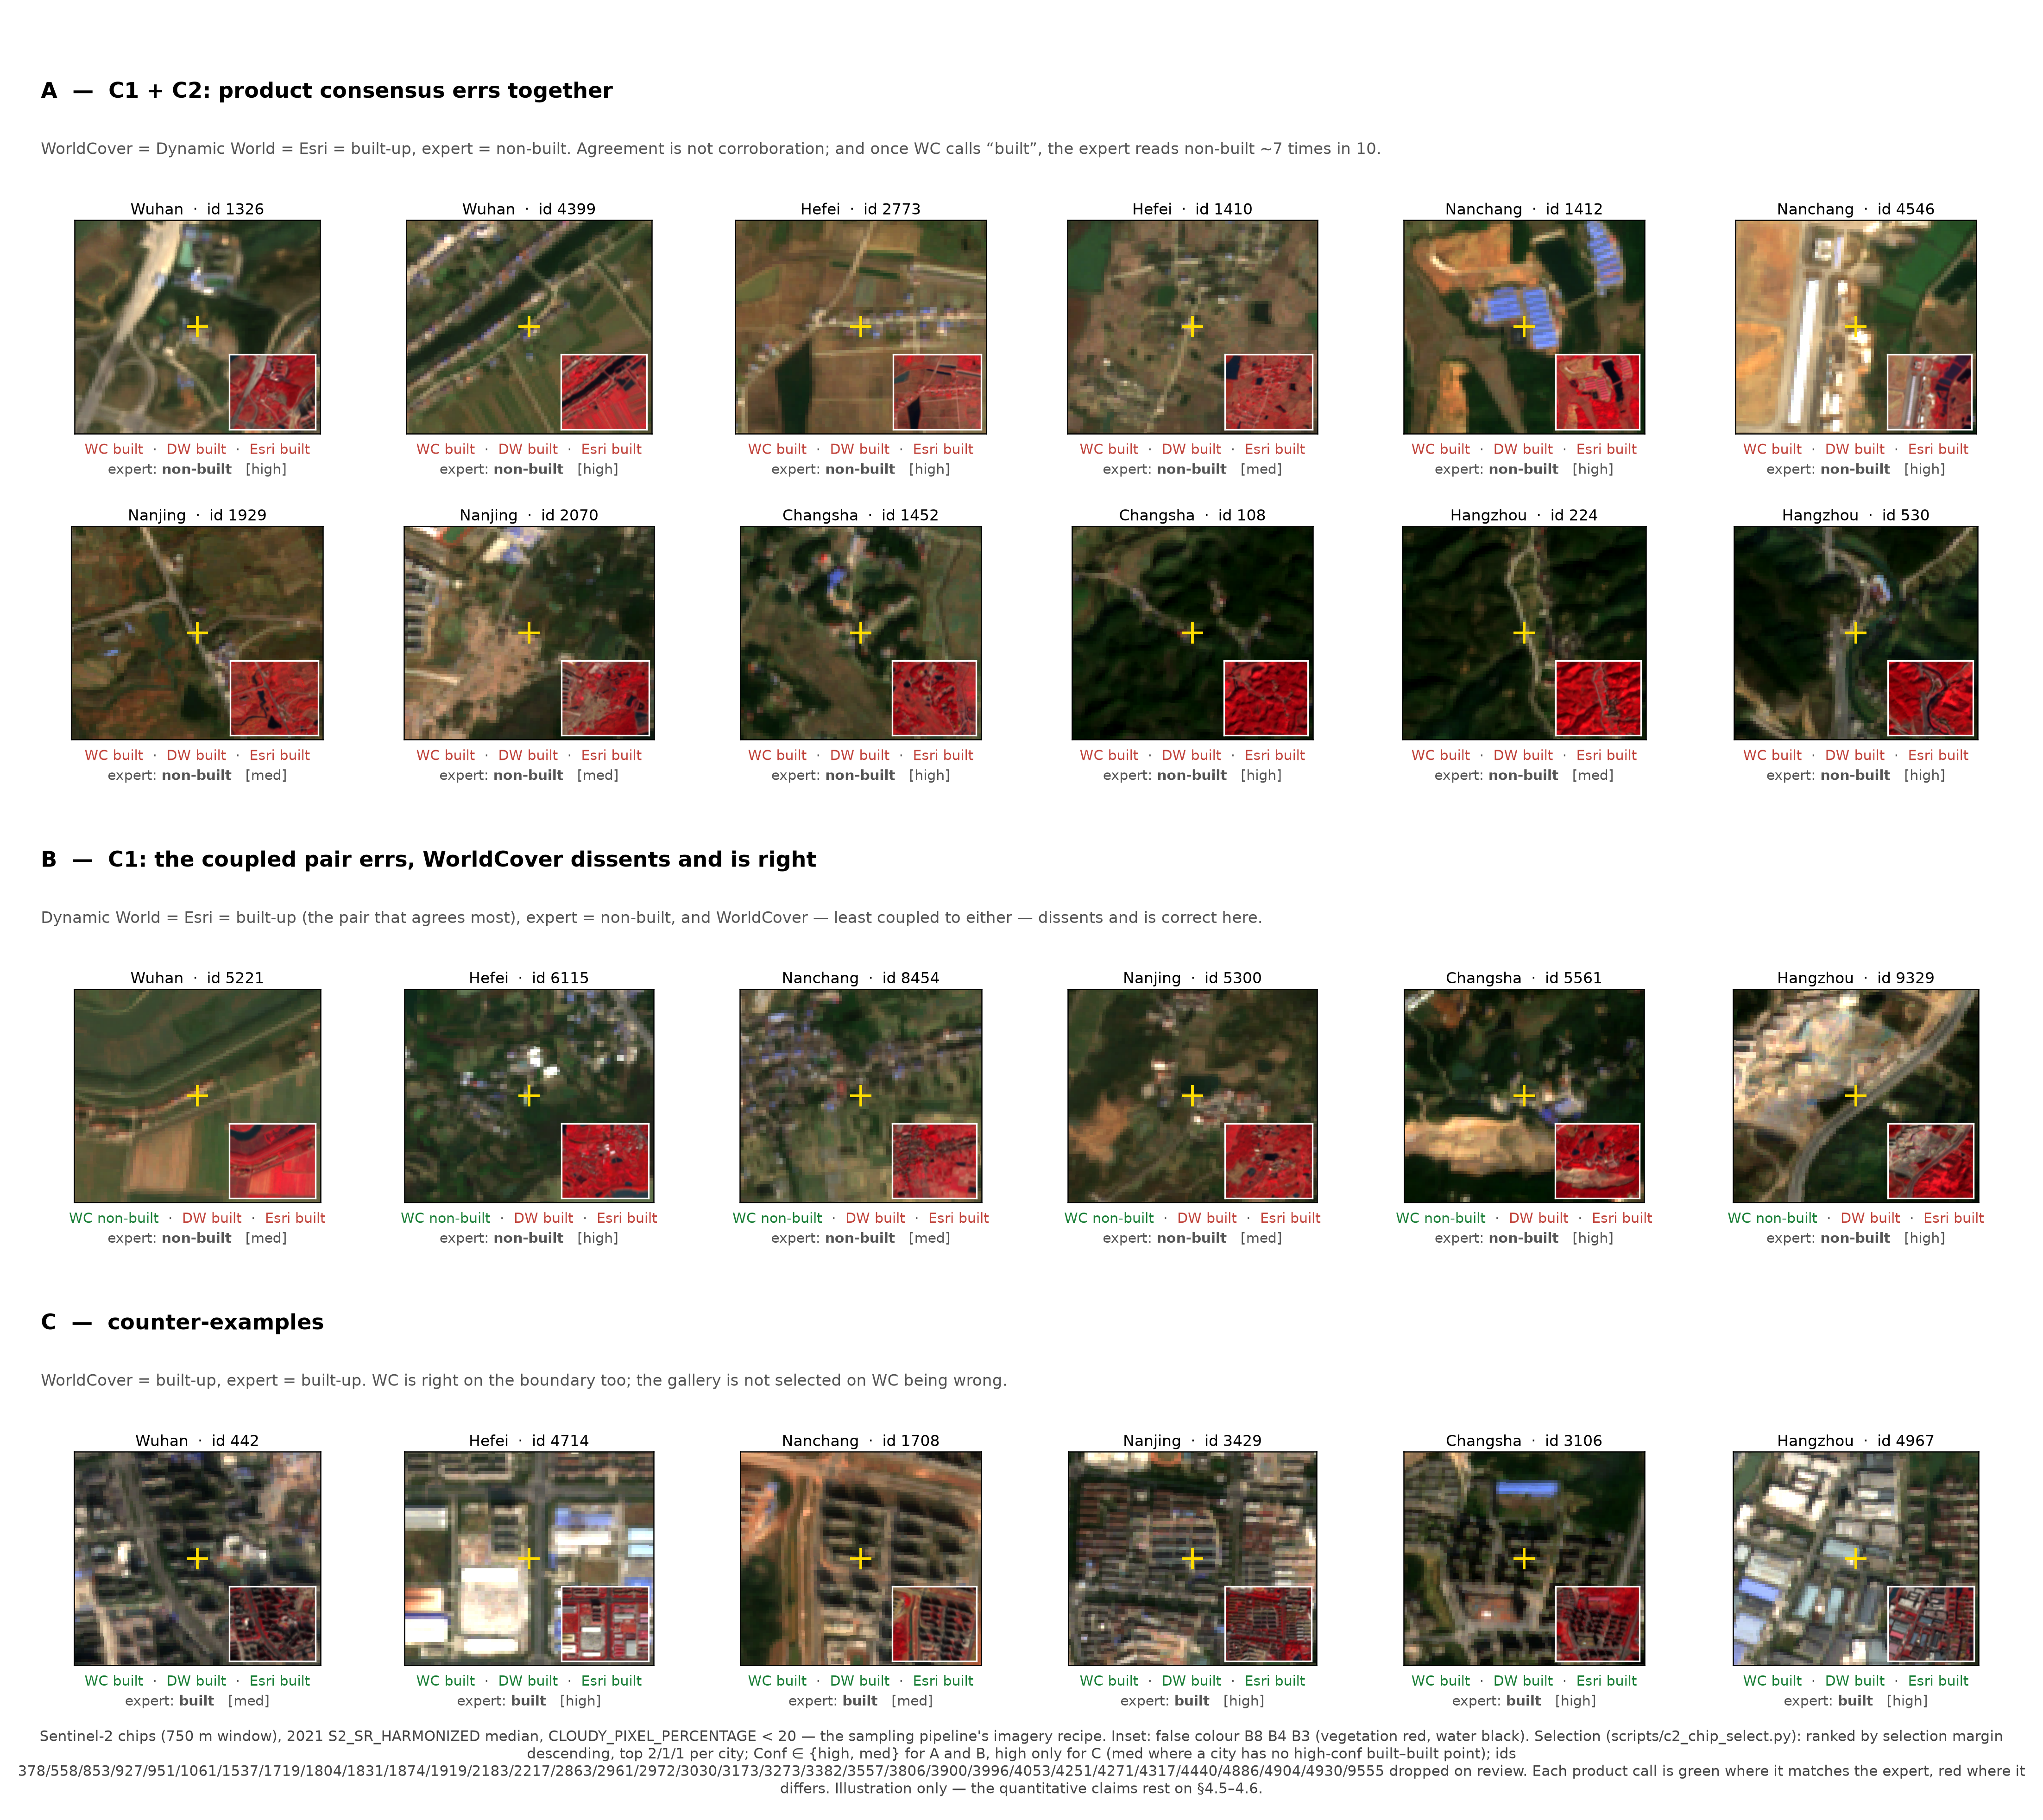
\includegraphics[width=\linewidth]{figures/FigureS5_c2_chips.png}
\caption{Twenty-four Sentinel-2 boundary chips (750~m window, true colour
with a false-colour NIR inset---vegetation red, water black), grouped as
(\textbf{A})~consensus error, (\textbf{B})~coupled-pair error,
(\textbf{C})~counter-examples, as described above. Each chip gives the
WorldCover / Dynamic World / Esri / expert calls, expert confidence, city and
point id; a product's call is printed in green where it matches the expert
and red where it differs, so the per-product pattern in each panel is
readable at a glance without checking the labels one by one. Selection rule,
confidence filter and exclusions detailed in the text above; illustration
only, the quantitative claim rests on Table~\ref{tab:T3}
(Section~\ref{sec:results-errordir}).\label{fig:S5chips}}
\end{figure}

%% ===================== REFERENCES ==============================
%% =====================================================================
%%  body/references.tex  --  internal bibliography
%%  Drop-in fragment; compiles only inside the MDPI Remote Sensing template.
%%
%%  MDPI "variant B" internal bibliography. Keep \externalbibliography{yes}
%%  in the preamble (the class default) -- it works with an inline
%%  thebibliography. Order = first citation order in the manuscript.
%%
%%  Entry data sources: memory/study-area-citations.md (DOIs web-verified
%%  2026-09-08/09) and docs/manuscript.md "References to insert".
%%
%%  2026-09-11 — external-review fix pass (Remote_Sensing_投稿评估.md), both
%%  confirmed via the Crossref API against the entry's own DOI:
%%  (1) yuan2026: volume was 105, Crossref gives 117 -- fixed, %VERIFY marker
%%  removed. (2) yang2021land: author block was "Yang, Y.; Li, H.; Qian, C.",
%%  which does not match any of the 12 real authors on this DOI (Crossref:
%%  Yi, Zhang, Zhang, Xing, Zhong, Liu, Lin, Zheng, Yang, Sun, Shi, Kang) --
%%  looks like a different reference's author block was pasted in. Replaced
%%  with the first 10 authors + "et al." (matches this bibliography's
%%  existing truncation convention, e.g. zanaga2022); bibitem label updated
%%  Yang et al. -> Yi et al. to match the real first author. %VERIFY marker
%%  removed.
%%
%%  2026-09-11 (2) — remaining 4 %VERIFY markers resolved via Crossref API
%%  against each entry's own DOI: (3) zhangroy2017: DOI confirmed correct
%%  (vol 197, pp 15-34, authors Zhang/Roy all match) -- marker removed, no
%%  content change. (4) wang2024a: author list was missing the last two of 8
%%  real authors (Crossref adds Wang, R.; Zong, J.) -- added; journal
%%  abbreviation confirmed as "GISci. Remote Sens." (was "GIScience Remote
%%  Sens.") per the journal's own ISO4 abbreviation -- fixed. (5) lu2026:
%%  author block was "Lu, N.; Chen, S.; Wang, Z.; Zhang, Y." -- Crossref shows
%%  the real co-authors are Jin, W.; Duan, X.; Zhang, M.; Zhang, C. (only the
%%  first author, Lu, was right) -- same wrong-author-block pattern as
%%  yang2021land above; volume 7 was already correct. (6) zhao2026: fully
%%  confirmed correct (all 6 authors, vol 19, article no. 2633840 match) --
%%  marker removed, no content change. No remaining %VERIFY markers in this
%%  bibliography.
%%
%%  2026-09-13 -- full re-check of all 23 entries against Crossref API (and
%%  DataCite for the Zenodo DOI); every DOI resolves and every author list,
%%  volume, and page/article number matches. Three entries had titles
%%  silently "corrected" away from the publisher's actual (slightly awkward)
%%  title text; restored to match the DOI record verbatim: (7) wang2024b:
%%  "high-resolution land cover products" -> "high-resolution global land
%%  cover products" (repeated "global" is in the published title, confirmed
%%  independently via Semantic Scholar). (8) yu2023: "...Yangtze River Based
%%  on the PSR Model" -> "...Yangtze River Base on the PSR Model" (published
%%  title omits the "d"; confirmed via Semantic Scholar). (9) karra2021:
%%  "Sentinel-2" -> "Sentinel 2" (no hyphen in the published title). Also
%%  (10) liao2025: author list was missing the 8th/last author, Chen, N.
%%  (Nengcheng Chen) -- added. fao2015gaul has no DOI (data citation); its
%%  catalog URL returned HTTP 502 on 2026-09-13 (checked 3x) -- likely a
%%  transient FAO server issue, not a dead link, but worth a final check
%%  before submission. landis1977/wilson1927/yule1900 have no DOIs listed
%%  (pre-DOI-era papers, MDPI style allows this) but content was cross-checked
%%  against Crossref search and is correct. No other discrepancies found.
%% =====================================================================

\reftitle{References}

\begin{thebibliography}{99}

\bibitem[Venter et al.(2022)]{venter2022}
Venter, Z.S.; Barton, D.N.; Chakraborty, T.; Simensen, T.; Singh, G.
Global 10 m Land Use Land Cover Datasets: A Comparison of Dynamic World, World
Cover and Esri Land Cover. \textit{Remote Sens.} \textbf{2022}, \textit{14}, 4101.
\href{https://doi.org/10.3390/rs14164101}{https://doi.org/10.3390/rs14164101}.

\bibitem[Xu et al.(2024)]{xu2024}
Xu, P.; Tsendbazar, N.-E.; Herold, M.; de Bruin, S.; Koopmans, M.; Birch, T.;
Carter, S.; Fritz, S.; Lesiv, M.; Mazur, E.; et al.
Comparative validation of recent 10 m-resolution global land cover maps.
\textit{Remote Sens. Environ.} \textbf{2024}, \textit{311}, 114316.
\href{https://doi.org/10.1016/j.rse.2024.114316}{https://doi.org/10.1016/j.rse.2024.114316}.

\bibitem[Yuan et al.(2026)]{yuan2026}
Yuan, S.; Liu, X.; Li, Y.; Hu, Y.; Huang, C.
Systematic underestimation of urban green space by global land cover products.
\textit{Urban For. Urban Green.} \textbf{2026}, \textit{117}, 129299.
\href{https://doi.org/10.1016/j.ufug.2026.129299}{https://doi.org/10.1016/j.ufug.2026.129299}.

\bibitem[Tuanmu and Jetz(2014)]{tuanmu2014}
Tuanmu, M.-N.; Jetz, W.
A global 1-km consensus land-cover product for biodiversity and ecosystem
modelling. \textit{Glob. Ecol. Biogeogr.} \textbf{2014}, \textit{23}, 1031--1045.
\href{https://doi.org/10.1111/geb.12182}{https://doi.org/10.1111/geb.12182}.

\bibitem[Zhang and Roy(2017)]{zhangroy2017}
Zhang, H.K.; Roy, D.P.
Using the 500 m MODIS land cover product to derive a consistent continental
scale 30 m Landsat land cover classification. \textit{Remote Sens. Environ.}
\textbf{2017}, \textit{197}, 15--34.
\href{https://doi.org/10.1016/j.rse.2017.05.024}{https://doi.org/10.1016/j.rse.2017.05.024}.

\bibitem[Wang et al.(2024a)]{wang2024a}
Wang, Y.; Sun, Y.; Cao, X.; Wang, Y.; Zhang, W.; Cheng, X.; Wang, R.; Zong, J.
Automatic training sample collection utilizing multi-source land cover products
and time-series Sentinel-2 images. \textit{GISci. Remote Sens.}
\textbf{2024}, \textit{61}, 2352957.
\href{https://doi.org/10.1080/15481603.2024.2352957}{https://doi.org/10.1080/15481603.2024.2352957}.

\bibitem[Wang et al.(2024b)]{wang2024b}
Wang, Y.; Xu, Y.; Xu, X.; Jiang, X.; Mo, Y.; Cui, H.; Zhu, S.; Wu, H.
Evaluation of six global high-resolution global land cover products over China.
\textit{Int. J. Digit. Earth} \textbf{2024}, \textit{17}, 2301673.
\href{https://doi.org/10.1080/17538947.2023.2301673}{https://doi.org/10.1080/17538947.2023.2301673}.

\bibitem[Chakraborty et al.(2024)]{chakraborty2024}
Chakraborty, T.C.; Venter, Z.S.; Demuzere, M.; Zhan, W.; Gao, J.; Zhao, L.;
Qian, Y. Large disagreements in estimates of urban land across scales and their
implications. \textit{Nat. Commun.} \textbf{2024}, \textit{15}, 9165.
\href{https://doi.org/10.1038/s41467-024-52241-5}{https://doi.org/10.1038/s41467-024-52241-5}.

\bibitem[Tong et al.(2025)]{tong2024pre}
Tong, X.-Y.; Dong, R.; Zhu, X.X.
Global high categorical resolution land cover mapping via weak supervision.
\textit{ISPRS J. Photogramm. Remote Sens.} \textbf{2025}, \textit{220}, 535--549.
\href{https://doi.org/10.1016/j.isprsjprs.2024.12.017}{https://doi.org/10.1016/j.isprsjprs.2024.12.017}.

\bibitem[Yi et al.(2021)]{yang2021land}
Yi, Y.; Zhang, C.; Zhang, G.; Xing, L.; Zhong, Q.; Liu, J.; Lin, Y.; Zheng, X.;
Yang, N.; Sun, H.; et al.
Effects of Urbanization on Landscape Patterns in the Middle Reaches of the
Yangtze River Region. \textit{Land} \textbf{2021}, \textit{10}, 1025.
\href{https://doi.org/10.3390/land10101025}{https://doi.org/10.3390/land10101025}.

\bibitem[Liao et al.(2025)]{liao2025}
Liao, S.; Wang, W.; Wang, C.; Ji, R.; Cui, A.; Chen, D.; Zhang, X.; Chen, N.
Land Use and Land Cover Change Assessment and Predictions in Flood Detention
Areas of Yangtze River Basin Based on AIF-HOM-PLUS Model. \textit{Remote Sens.}
\textbf{2025}, \textit{17}, 1857.
\href{https://doi.org/10.3390/rs17111857}{https://doi.org/10.3390/rs17111857}.

\bibitem[Yu et al.(2023)]{yu2023}
Yu, S.; Yang, L.; Song, Z.; Li, W.; Ye, Y.; Liu, B.
Measurement of Land Ecological Security in the Middle and Lower Reaches of the
Yangtze River Base on the PSR Model. \textit{Sustainability} \textbf{2023},
\textit{15}, 14098.
\href{https://doi.org/10.3390/su151914098}{https://doi.org/10.3390/su151914098}.

\bibitem[Tong et al.(2024)]{tong2024land}
Tong, C.; Jin, Y.; Liang, B.; Ye, Y.; Bao, H.
A Comprehensive Framework for Monitoring and Providing Early Warning of Resource
and Environmental Carrying Capacity Within the Yangtze River Economic Belt Based
on Big Data. \textit{Land} \textbf{2024}, \textit{13}, 1993.
\href{https://doi.org/10.3390/land13121993}{https://doi.org/10.3390/land13121993}.

\bibitem[Lu et al.(2026)]{lu2026}
Lu, N.; Jin, W.; Duan, X.; Zhang, M.; Zhang, C.
Long-term changes in dry-season water bodies and lake-littoral land-cover
structure of typical lakes in the middle-lower Yangtze and Huai River basins,
China (1999--2019). \textit{Front. Remote Sens.} \textbf{2026}, \textit{7},
1869619.
\href{https://doi.org/10.3389/frsen.2026.1869619}{https://doi.org/10.3389/frsen.2026.1869619}.

\bibitem[Zhao et al.(2026)]{zhao2026}
Zhao, Y.; Zhang, X.; Duan, X.; Zou, H.; Liu, D.; Wan, R.
RoLaSTIM: a novel method for lakeshore type identification and utilization rate
assessment. \textit{Int. J. Digit. Earth} \textbf{2026}, \textit{19}, 2633840.
\href{https://doi.org/10.1080/17538947.2026.2633840}{https://doi.org/10.1080/17538947.2026.2633840}.

\bibitem[FAO(2015)]{fao2015gaul}
Food and Agriculture Organization of the United Nations.
\textit{The Global Administrative Unit Layers (GAUL) 2015, Second-Level
Administrative Units}; FAO: Rome, Italy, 2015. Available online:
\url{https://data.apps.fao.org/catalog/dataset/global-administrative-unit-layers-gaul-2015}
(accessed on 20 July 2026; the previously cited
\url{https://data.apps.fao.org/map/catalog/} now 502s, re-verified
2026-09-15);
Google Earth Engine asset \href{https://developers.google.com/earth-engine/datasets/catalog/FAO_GAUL_2015_level2}{\path{FAO/GAUL/2015/level2}}.

\bibitem[Gorelick et al.(2017)]{gorelick2017}
Gorelick, N.; Hancher, M.; Dixon, M.; Ilyushchenko, S.; Thau, D.; Moore, R.
Google Earth Engine: Planetary-scale geospatial analysis for everyone.
\textit{Remote Sens. Environ.} \textbf{2017}, \textit{202}, 18--27.
\href{https://doi.org/10.1016/j.rse.2017.06.031}{https://doi.org/10.1016/j.rse.2017.06.031}.

\bibitem[Zanaga et al.(2022)]{zanaga2022}
Zanaga, D.; Van De Kerchove, R.; Daems, D.; De Keersmaecker, W.; Brockmann, C.;
Kirches, G.; Wevers, J.; Cartus, O.; Santoro, M.; Fritz, S.; et al.
\textit{ESA WorldCover 10 m 2021 v200}; Zenodo, 2022.
\href{https://doi.org/10.5281/zenodo.7254221}{https://doi.org/10.5281/zenodo.7254221}.

\bibitem[Brown et al.(2022)]{brown2022}
Brown, C.F.; Brumby, S.P.; Guzder-Williams, B.; Birch, T.; Hyde, S.B.;
Mazzariello, J.; Czerwinski, W.; Pasquarella, V.J.; Haertel, R.;
Ilyushchenko, S.; et al. Dynamic World, Near real-time global 10 m land use land
cover mapping. \textit{Sci. Data} \textbf{2022}, \textit{9}, 251.
\href{https://doi.org/10.1038/s41597-022-01307-4}{https://doi.org/10.1038/s41597-022-01307-4}.

\bibitem[Karra et al.(2021)]{karra2021}
Karra, K.; Kontgis, C.; Statman-Weil, Z.; Mazzariello, J.C.; Mathis, M.;
Brumby, S.P. Global land use / land cover with Sentinel 2 and deep learning. In
Proceedings of the IGARSS 2021 IEEE International Geoscience and Remote Sensing
Symposium, Brussels, Belgium, 11--16 July 2021; pp. 4704--4707.
\href{https://doi.org/10.1109/IGARSS47720.2021.9553499}{https://doi.org/10.1109/IGARSS47720.2021.9553499}.

\bibitem[Landis and Koch(1977)]{landis1977}
Landis, J.R.; Koch, G.G.
The measurement of observer agreement for categorical data.
\textit{Biometrics} \textbf{1977}, \textit{33}, 159--174.

\bibitem[Wilson(1927)]{wilson1927}
Wilson, E.B.
Probable inference, the law of succession, and statistical inference.
\textit{J. Am. Stat. Assoc.} \textbf{1927}, \textit{22}, 209--212.

\bibitem[Yule(1900)]{yule1900}
Yule, G.U.
On the association of attributes in statistics: with illustrations from the
material of the childhood society, \&c. \textit{Philos. Trans. R. Soc. Lond. A}
\textbf{1900}, \textit{194}, 257--319.

\end{thebibliography}

\end{document}
